\documentclass{article}
\usepackage{float}
\usepackage{graphicx}
\usepackage{caption}
\usepackage{subfig}
\usepackage{lipsum}
\usepackage{tikz}
\usepackage{eso-pic}
\usepackage{changepage}
\usepackage{xcolor}
\usepackage{afterpage}
\usepackage[document]{ragged2e}
\usepackage[none]{hyphenat}
\usepackage[margin=1in,footskip=0.25in]{geometry}
\usepackage{array}
% \usepackage{l3kernel}
% \usepackage{l3packages}
\usepackage{siunitx}
\usepackage{color,soul}
\usepackage{placeins}
\usepackage{microtype}
\usepackage[backend=biber]{biblatex}
\usepackage[hidelinks]{hyperref}
\usepackage[toc,page]{appendix}
%\usepackage[toc]{glossaries}
\usepackage[subfigure]{tocloft}
\usepackage{rotating}
\usepackage[printwatermark]{xwatermark}
% \usepackage[table,xcdraw]{xcolor}
\usepackage{xcolor}
\hypersetup{
	colorlinks,
	linkcolor={black!50!black},
	citecolor={blue!50!black},
	urlcolor={blue!80!black}
}

\cftsetindents{subsection}{.25in}{.4in}

\usepackage[flushleft]{threeparttable}
\newcolumntype{C}[1]{>{\centering\let\newline\\\arraybackslash\hspace{0pt}}m{#1}}

\definecolor{ULred}{HTML}{872434}

\usepackage{chngcntr}
\counterwithin{table}{section}
\counterwithin{figure}{section}

\pdfoptionpdfminorversion=6
%\addbibresource{FireAttackReport.bib}

\setlength{\parskip}{1em}

% ******* REMOVE COMMENTS AND PLACE GLOSSARY.TEX IN ROOT DIRECTORY TO ADD GLOSSARY, SEE END FOR ADDITIONAL LINES TO UNCOMMENTS *******
%
%\loadglsentries{glossary.tex}
%
%\makeglossaries

% ******* REMOVE COMMENTS ON THIS BLOCK TO ADD DRAFT TO REPORT ********
% \newsavebox\mybox
% \savebox\mybox{\tikz[color=gray,opacity=0.5]\node{DRAFT};}
% \newwatermark*[
% allpages,
% angle=65,
% scale=15,
% xpos=-65,
% ypos=20
% ]{\usebox\mybox}

\begin{document}
	
	\begin{titlepage}
		
		\pagecolor{ULred}\afterpage{\nopagecolor}
		

		\AddToShipoutPictureFG*{\AtPageUpperLeft{\raisebox{-\height}{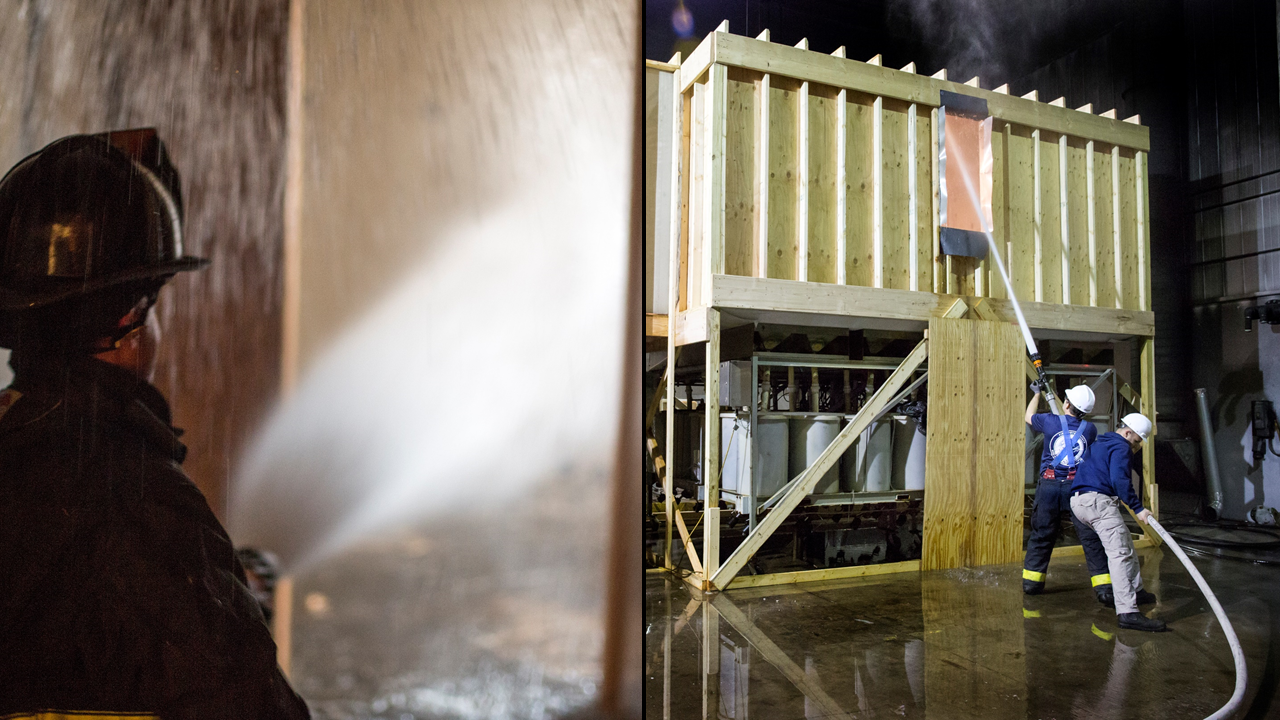
\includegraphics[width=7in]{Figures/General/TitlePagePhotoNew}}}} 

			\vspace*{20\baselineskip} 

		\huge
		\begin{adjustwidth}{-0.5in}{-0in}
		\color{white}
		\textbf{Study of the Impact of Fire Attack \\ Utilizing Interior and Exterior Streams \\ on Firefighter Safety and Occupant Survival}
		\end{adjustwidth}
		\huge
		\begin{adjustwidth}{-0.5in}{-0in}
		\color{white}
		\textbf{Part I: Air Entrainment and Water Distribution}
		\end{adjustwidth}
		\begin{adjustwidth}{-0.5in}{}
		\color{white}
		\vspace{.2\baselineskip}
		\large
		Stephen Kerber \\
		Director \\
		UL Firefighter Safety Research Institute \\
		\vspace*{.5\baselineskip}
		Robin Zevotek \\
		Lead Engineer \\
		UL Firefighter Safety Research Institute \\ 
		\vspace*{.5\baselineskip}
		Keith Stakes \\
		Research Engineer \\
		UL Firefighter Safety Research Institute \\
		\vspace*{.8\baselineskip}	
		\today
		\vspace*{.8\baselineskip}
		\begin{figure}[h]
			\hspace*{-0.5in}
\includegraphics[width=0.75in]{../0_Images/ULLogoWhite.pdf}
		\end{figure}
		\end{adjustwidth}
	\end{titlepage}

\begin{center}
	DISCLAIMER\\
	\vspace*{\baselineskip}
	\begin{adjustwidth}{-0.25in}{-0.25in}
		In no event shall UL be responsible to anyone for whatever use or non-use is made of the information contained in this Report and in no event shall UL, its employees, or its agents incur any obligation or liability for damages including, but not limited to, consequential damage arising out of or in connection  with the use or inability to use the information contained in this Report. Information conveyed by this Report applies only to the specimens actually involved in these tests. UL has not established a factory Follow-Up Service Program to determine the conformance of subsequently produced material, nor has any provision been made to apply any registered mark of UL to such material. The issuance of this Report in no way implies Listing, Classification or Recognition by UL and does not authorize the use of UL Listing, Classification or Recognition Marks or other reference to UL on or in connection with the product or system.
	\end{adjustwidth}
\end{center}

\begin{center}
	ACKNOWLEDGEMENTS
\vspace*{\baselineskip}
\begin{adjustwidth}{-0.25in}{-0.25in}
This work was funded through a grant from the Department of Homeland Security's Assistance to Firefighters Grant Program under the Fire Prevention and Safety Grants: Research and Development. Without this critical funding and support, this vital fire service research would not be possible.

\vspace*{\baselineskip}

\begin{center}
	
\includegraphics[width=0.28\textwidth]{Figures/General/DHS}
\end{center}

\clearpage

In order to better design and implement the experiments for the Fire Attack study, UL - FSRI has gathered a group of fire service experts from across the world with knowledge in fire suppression and the impact of interior and exterior fire streams. The individuals below provided direction for the project, assisting in planing the experiments, witnessing the testing, and developing concrete conclusions. Their tireless support and effort make this project relevant to the fire service across the world. 

\vspace*{\baselineskip}

\renewcommand{\arraystretch}{1.5}

\begin{table}[H]
	\centering
	\begin{tabular}{|c|c|}
		\hline
		\bf{Name} & \bf{Fire Department} \\ \hline \hline
		Chad Green & Anchorage Fire Department \\ \hline
		Chad Christensen & Los Angeles County Fire Department \\ \hline
		Dennis Legear & Oakland Fire Department \\ \hline
		Tony Carroll & Washington DC Fire Department \\ \hline
		Jordan Mohr & Sedgwick County Fire District 1 \\ \hline
		Samuel Hittle & Wichita Fire Department \\ \hline
		John Gallagher & Boston Fire Department \\ \hline
		Josh Hummel & Howard County Department of Fire and Rescue Services \\ \hline
		Matt Carrigan & Montgomery County Fire and Rescue Service \\ \hline
		Kelly Hanink & Eden Prairie Fire Department \\ \hline
		Jason Floyd & Las Cruces Fire Department \\ \hline
		Jerry Knapp & West Haverstraw (NY) Fire Department \\ \hline
		Ray McCormack & Fire Department of New York \\ \hline
		Jacob Hoffman & Toledo Fire/Rescue Department \\ \hline
		Steve Pegram & Goshen Township Fire and EMS \\ \hline
		Danny Doyle & Pittsburgh Fire Department \\ \hline
		Nick Martin & Columbia Fire Department \\ \hline
		Albert Castillo & Houston Fire Department \\ \hline
		Aaron Fields & Seattle Fire Department \\ \hline
		Steve Brisebois & Montreal Fire Department \\ \hline
		Hans Neiling & Zuid Limburg Fire \\ \hline
		John McDonough & New South Wales Fire Department \\ \hline
		John Chubb & Dublin Fire Brigade \\ \hline		 		  
	\end{tabular}
	\caption*{Fire Service Technical Panel}
\end{table}

\end{adjustwidth}
\end{center}

\clearpage

\renewcommand{\abstractname}{Abstract}
\setlength{\emergencystretch}{5pt}

\begin{abstract}

As research continues into how fire department interventions affect fire dynamics in the modern fire environment; questions continue to arise on the impact and implications of interior versus exterior fire attack on both firefighter safety and occupant survivability. Previous research into various types of fire ground ventilation, flow paths, and exterior fire streams has provided the fire service with a more in-depth understanding of fire dynamics in addition to causing concern about certain fire attack methods stemming from differing traditions and myths. This knowledge gap and lack of previous research in this area has driven the need for further study into fire department interventions at structure fires with a focus on hose streams and suppression tactics. Statistics show that both firefighters and building occupants continue to loose their lives due to fire. As such, research into the various methods of fire attack will allow a broader understanding of how firefighter interventions on the fire ground can impact the outcome of both life safety and property protection. 

\vspace*{\baselineskip}

This study will build and expand upon the fire research conducted to date by analyzing how firefighting tactics, specifically suppression methods, affect the thermal exposure and survivability of both firefighters and buidling occupants in addition to impacting fire behavior in structures. The purpose of this study is to improve firefighter safety, fireground tactics, and the knowledge of fire dynamics by providing the fire service with credible scientific information, developed from both water flow and full-scale fire testing, in representative single family homes. The project will be comprised of 3 parts:
\vspace*{\baselineskip}
\begin{itemize}
	\item Part I: Air Entrainment and Water Distribution.
	\item Part II: Full-Scale Residential Fire Experiments.
	\item Part III: Acquired Structure Fire Testing.
	\end{itemize}
\vspace*{\baselineskip}

This report details the results and analysis from the air entrainment and water distribution experiments. These tests were conducted without the presence of fire in order to gain a basic understanding of air flow and water flow before Parts II and III of the study were conducted as full-scale fire experiments. Each test was designed to quantify the air entrainment in hose streams and determine where water is distributed within compartments by evaluating the differences caused by various application methods, hose stream types, nozzle movements, pressures/flow rates, and stream locations and elevation angles. Over 150 tests were conducted in Part I of the overall study. Results from these experiment series were analyzed and reviewed with assistance from our technical panel. These results were summarized and can be seen below:

\vspace*{\baselineskip}
\noindent \bf{Air Entrainment} -
\normalfont
\begin{itemize}
	\item Air entrainment is dependent on hose stream type. (smooth bore, straight stream, fog)
	\item Air entrainment is dependent on structure size, compartmentation, and ventilation configurations.
	\item Increases in nozzle movement increase overall air entrainment.
	\item Different nozzle movement patterns have little effect on overall air entrainment. (O, T, Z, inverted U)
	\item Air entrainment, either into or out of the structure, is dependent on the horizontal distance of the nozzle to the ventilation opening.
	\end{itemize}
\vspace*{\baselineskip}
\noindent \bf{Water Distribution} -
\normalfont
\begin{itemize}
	\item Water distribution is dependent on hose stream type. (smooth bore, straight stream, fog)
	\item Water distribution is dependent on stream elevation angle within a compartment.
	\item Varying water pressure at the nozzle and flow rate can affect the total amount of water applied to a given area; however, the distribution location can remain constant.
	\item Deflecting the hose stream off the ceiling or opposite wall of a compartment can coat the surfaces while applying little water to the center of the room.
	\end{itemize}
\vspace*{\baselineskip}

\end{abstract}

\newpage

\tableofcontents

\newpage

\section{Background}

Recent fire service research has highlighted the importance of applying water to the fire as quickly as possible. This tactical consideration has highlighted a knowledge gap and increased the interest in better understanding the impact of water applied as part of an interior or exterior attack. Many variables exist in fire attack that impact firefighter effectiveness and victim survivability including stream placement, the time required to get water on the fire, stream type, stream movement, air entrainment, steam development, hot gas cooling and contraction, and position of flow paths. The most important firefighting tool for many years at structure fires has been their hoseline; however, many questions have arisen as more research shows the impact of ventilation, flow paths, and exterior fire streams. Whether a fire attack crew chooses to apply water as part of an interior attack or as part of an exterior or ``transitional attack," they need to know what impact their stream has on the fire environment ahead of them. This is difficult on the fire ground because visibility is commonly limited and therefore most experience and first-hand accounts are from behind the nozzle. This results in beliefs about conditions (e.g. temperature) ahead of the nozzle team and the impact of their tactics on victim survivability; but knowledge of the actual impact has yet been researched. Additionally, when the fire is ultimately suppressed, there is no assurance the attack was conducted in the most effective, efficient, and safe manner even if the experience gained suggests that it was. Fire service adages such as ``don’t put water on smoke,'' ``you will steam the victims,'' and ``fog nozzles always disrupt the thermal layer'' have been passed on from generation to generation with little context or substantiation. Without the context, these concepts get treated like rules and can severely limit firefighters understanding of fire suppression.

Current fire training curriculum defines 3 fire attack methods: direct attack, indirect attack, and combination attack. Direct attack involves the discharge of water directly onto the burning fuel. Indirect attack involves directing the stream toward the ceiling of a compartment in order to generate a large amount of steam in order to cool the compartment. Converting the water to steam displaces oxygen, absorbs the heat of the fire and cools the hot gas layer sufficiently for firefighters to safely enter and make a direct attack. Combination attack extinguishes a fire by using both a direct and indirect attack. Another technique to safely approach a fire that cannot be reached with a direct attack is gas cooling. Gas cooling provides a buffer zone around the attack team but the larger the compartment, the less the impact on cooling the hot gas layer. Gas cooling must be a continuous process while advancing toward a shielded fire. Techniques for effective gas cooling and the upper limit of the volume where gas cooling is effective is not well known.  

\hl{*** ADD BACKGROUND SPECIFIC TO AIR ENTRAINMENT AND ADD ***}
\hl{DAN TO ORGANIZE}

Fire suppression effectiveness and firefighter safety are not achieved by water flow rate alone, but by appropriate use of a given flow rate under specific fire ground conditions. A flow rate must meet the critical flow rate to extinguish a fire depending on the heat release rate and should be higher to reduce the time to extinguishment. Drastically exceeding the critical flow rate has less known impact on time to extinguishment but has a significant impact on the total amount of water used. To-date, there is little data to connect the critical flow rate to firefighter safety. However, it has been estimated that only 5 to 10 percent of water applied during fire attack contributes to extinguishment. It is difficult for firefighters to realize the the efficiency of various hose stream techniques due to poor visibility on the fireground. However, by developing data in realistic structures, fuel sources, and fire scenarios, important inferences may be developed relative to different hose stream techniques, and use of water.

\clearpage

\section{Objectives and Technical Plan}

\subsection {Objectives}

The purpose of this part to the overall study was to provide the fire service with scientific based knowledge on the impact of hose streams during interior and exterior fire attack on firefighter safety and trapped occupants to improve training and decision making on the fire ground. This was accomplished with the completion of the following objectives:

\begin{itemize}
	\item Improve firefighter safety by increasing knowledge of fire suppression.
	\item Develop knowledge of hose streams applied during an interior and exterior fire attack and its impact on firefighter safety and victim survivability.
	\item Understand where water goes and how air flows during interior and exterior fire attack utilizing common equipment, practices, and tactics.
	\item Gain understanding of the impact of water streams depending on the volume of the fire compartment/structure.
	\item Bring the `Science to the Streets' by transferring science based conclusions founded on experimental results that can be incorporated into firefighting standard operating procedures.
	\end{itemize}

% All five of the Technology \& Fire Service Science issues facing the fire service determined during the 2nd National Fire Service Research Symposium \cite{NFFF} were incorporated into this study.

\clearpage

\subsection{Technical Plan}

Part I to the study consisted of the following tasks. 

\begin{itemize}

\item \bf{Task 1 - Design of Experiments}
\normalfont
\vspace*{\baselineskip}

Task 1 is the design of the experiments. In this task, UL - FSRI's project engineers will work closely with the technical panel to ensure fire service concerns are addressed and that the results will be of great benefit to the end users. All experimental variables, equipment, personnel, infrastructure, and other resources will be evaluated to determine the best set of experiments to get the most for the investment and provide the largest return to the fire service community. Variables such as types of nozzles, flow rates, nozzle pressures, hose stream types, stream elevation angles, ventilation parameters, and timing of tactics will be discussed and selected.  
\vspace*{\baselineskip}

\item \bf{Task 2 - Test Fixture Design}
\normalfont
\vspace*{\baselineskip}

Task 2 is the design of the test fixtures to be used in the experiments. There will be a separate main test fixture for each test series. The air entrainment experiments will be utilizing an exisiting structure at the Delaware County Emergency Services Training Facility repurposed for this study and the water distribution structure will be constructed within a lab space inside UL`s Large Fire Facility. The structures and compartments incorporated into this study are representative in both size and construction type of the structures utilized in the full-scale fire experiments for Parts II and III of the study. These fixtures are similar in construction type and size to the structures built for the three previous ventilation research grants and will therefore allow continuity of previous results to expand our knowledge. Additional test fixture details are provided in the detailed report below.
\vspace*{\baselineskip}

\item \bf{Task 3 - Conduct Experiments}
\normalfont
\vspace*{\baselineskip}

\subitem \bf{Task 3A:  Water Flow Mapping (Interior and Exterior Applications)}
\normalfont
\vspace*{\baselineskip} 

Methodology: Conduct a series of experiments in a compartment constructed to determine where water goes once discharged from fire department nozzles during a simulated interior fire attack and exterior fire attack. The ability to suppress a fire safely and efficiently is dependent on how much water absorbs energy from the fire and what surfaces are cooled. A combination of water mapping techniques that are commonly used for characterizing sprinkler sprays will be utilized to determine flow distribution. The compartment will be of similar size to the fire rooms in the full-scale fire experiments so that the results can be linked.

Water will be flowed utilizing common fire department nozzles with 3 hose stream types (combination nozzle in straight stream, combination nozzle in narrow fog, and a smooth bore nozzle). Different nozzle techniques that are commonly taught to firefighters and utilized in practice will be evaluated such as circular motions, various patterns, flowing off the ceiling, and flowing ahead. Common flow rates for each nozzle will be used during the experiments. We will also construct a prop to aid in water delivery to distribute the water in a repeatable manner that would be done by firefighters in the field. Several experiments will be done to also examine repeatability.  

Measurements: The actual delivered density apparatus (described later) will be used to determine water distribution. 
\vspace*{\baselineskip}

\clearpage

\subitem \bf{Task 3B:  Air Flow and Pressure Experiments}
\normalfont
\vspace*{\baselineskip}

Methodology: Conduct air flow and pressure experiments in specific test fixtures prior to the introduction of any fire. Different hose streams and nozzle movement techniques entrain different amounts of air which can greatly impact fire dynamics, firefighter safety, and victim survivability. The same nozzles, hose stream types, and nozzle movement techniques from the water distribution experiments will be used and the amount of air flow generated in the structure will be measured. Different flow paths will also be established to see their impact such as having a ventilation point ahead of the hoseline when compared to having no ventilation opening ahead. We will also examine air movement generated by both 1 3/4~in. and 2 1/2~in. hoselines in addition to flows from portable and master-stream devices.

Measurements: During each of these experiments, velocities will be measured with bidirectional probes attached to differential pressure transducers. 
\vspace*{\baselineskip}

\item \bf{Task 4 - Data Compilation and Analysis}
\normalfont
\vspace*{\baselineskip}

Task 4 is the compilation and analysis that will be conducted by UL - FSRI engineers to make the data usable by the fire service community. The data will be organized in graphs that will be reviewed by the technical panel in preparation for the final report. The focus of the analysis will be to quantify air entrainment in hose streams and the location of where water is distributed during suppression. In addition, conclusions will be developed in conjunction with the fire service technical panel supported by data and subsequent analysis.
\vspace*{\baselineskip}

\item \bf{Task 5 - Develop Final Project Report}
\normalfont
\vspace*{\baselineskip}

Task 5 is the development of the final report that details all of the experiments and results. The report will be provided to DHS and made publicly available via UL - FSRI's website for the fire service, www.ULfirefightersafety.com to serve as a reference for future research. The conclusions developed with the technical advisory panel will be a focus within the report. A fire service summary report at the conclusion of the remainder of the study will also be written and disseminated to include critical information for firefighter safety.
\vspace*{\baselineskip}

\end{itemize}

\clearpage

\subsection{Limitation and Scope}

The purpose is to quantify the amount of air entrainment in hose streams given certain parameters as well as determine where water is distributed within a compartment. This is all without fire involvement in order to provide a baseline understanding before moving forward with the remainder of the study. This baseline knowledge is intended to bridge the gap in the fire service understanding about the use of various nozzles, hose stream types, nozzle movements, and advancement techniques in specific scenarios. Knowing how hose streams affect air movement and how water is distributed can allow for better decision making capabilities across the fire service when it comes to use during an actual emergency incident.

When analyzing the air entrainment and water distribution, equipment from various manufacturers was tested. For the purpose of the study, the companies will be referred to as Manufacturer 1, Manufacturer II, and Manufacturer III. The air entrainment experiments yielded results that showed little to no difference among the various manufacturers. Therefore, a single manufacturer was chosen for the remainder of Part I of the study. More specifically, Part I of the study is not intended to purchasing of one type of nozzle over another.

The intent of the air entrainment experiments was to determine how much air hose streams entrain. This involved several components:

\begin{itemize}
	\item Does the hose stream type (smooth bore versus straight stream versus narrow fog) effect air entrainment?
	\item Does the amount of air entrainment vary dependent on manufacturer given set flow rates/pressures?
	\item How do different building geometries, compartment layouts, and ventilation configurations effect air entrainment?
	\item Do various nozzle movements effect air entrainment (fixed, sweeping, O, T, Z, inverted U)?
	\item Does the distance from a ventilation opening effect the air entrainment?

\end{itemize}

Additionally, the intent of the water distribution experiments was to determine where water goes within a compartment. In order to answer this question, the tests considered the following:

\begin{itemize}
	\item Does interior versus exterior attack effect water distribution?
	\item Does the hose stream type (smooth bore versus straight stream versus narrow fog) effect water distribution? 
	\item Does the hose stream elevation angle effect water distribution?
	\item Does adjusting the flow rates/pressures of the nozzles effect water distribution? 
	\item Do various nozzle movements effect water distribution (fixed, sweeping, O)?
	\item How does a first floor exterior attack effect the water distribution when compared to a second floor exterior attack?
\end{itemize}

For the purpose of these experiments we utilized the same structure throughout all of the air entrainment experiments. The water distribution testing utilized another structure, which also remained the same for the duration of those experiments. The only component of the firefighting equipment that was varied among the tests was the nozzle, and sometimes the hoseline size. The hoseline diameter was either 1 3/4~in. or 2 1/2~in. and was always 200~ft. in length. By creating some aspects that were not varied and by bounding other variables, we ensured that all aspects of the air entrainment and water distribution were examined as a baseline for further future evaluation in different structures with different conditions.

\clearpage

\section{Previous Literature}

At the start of the study, a literature review was performed to identify and analyze the following:

\begin{itemize}
	\item Previous research in the field of air entrainment, water distribution, and fire suppression.
	\item Both past and current fire suppression tactics.
	\item Knowledge gaps in fire suppression operations. (choice of tactics, myths, traditions, etc.) 
\end{itemize}

The following section outlines some of the material as it relates to the fire attack study. The literature review encompassed past research work, various articles in fire service publications, fire service training manuals, as well as fire department standard operating procedures to highlight some of the critical areas of information which drove the project at hand.

\subsection{Literature Overview}

\hl{DAN TO ADD/ORGANIZE}

Hose, nozzles and water have been used by the fire service for hundreds of years. Despite their frequent use, there has been little scientific research conducted on the effective use of these tools for fire suppression. It is common in the fire service to find discussions about which nozzle is better or which flow rate is required for what sized fire but this is based on experience and usually not science. 

In 1950 Chief Lloyd Layman presented a paper titled “Little Drops of Water” at the Fire Department Instructors Conference. He introduced what he called indirect method of attack to suppress interior building fires by using the heat absorbing properties of expanding and condensing steam, produced in great quantities by fog streams. The conclusions were based on Coast Guard experiments that Layman was in charge of conducting at the Coast Guard Firefighting School at Fort McHenry in Baltimore, MD. Layman continued his experiments after he returned to his position as fire chief in Parkersburg, WV where he applied his tactic in building fires.  This research had a very large impact on the fire service and their suppression techniques to this day. 

Throughout the 1950’s a National Committee began conducting experiments to collect data on the growth and behavior of interior fires and how to most effectively suppress them. Keith Royer and Bill Nelson were members of this committee, and as the heads of the firemanship training program at the Iowa State University’s Engineering Extension, they collected and analyzed data from hundreds of experimental fires. Through this research the fire service was taught about fire behavior and how to suppress fire with a combination fire attack. They examined the amount of heat generated by common fuels, the heat absorbing capacity of water, the impact of compartment volume during suppression and they developed the Iowa formula. The Iowa formula or critical rate of flow formula is still used today and it determines the amount of water needed to control a fire in the largest open space within a structure by dividing the cubic foot volume of the space by 100.

While the physics of fire development has not changed over time, the fire environment for specifically the single family home has evolved. Several factors including home size, geometry, contents and construction materials have changed significantly over the past 50 or more years. Each of these factors has impacted firefighter and occupant safety. Faster fire propagation, shorter times to flashover, rapid changes in fire dynamics and shorter escape times all impact fire service suppression techniques and effectiveness. Many of the variables in Royer and Nelson’s analysis have changed and more research is needed to see how suppression techniques used in the 1950’s with 1950’s fuel loads and firefighting tools translates to today’s firefighter safety and effectiveness.

Beginning in 1994, the Naval Research Laboratory carried out a series of full-scale fire experiments to compare straight stream attack versus fog pattern attack. These experiments were conducted on the Navy ship ex-USS Shadwell with a fire volume of approximately 110~m$^3$. In these experiments one 60 degree fog pattern was applied at a 45 degree angle into the smoke layer. They examined cooling effects, steam generation and thermal layer disruption. Their experiments examined shielded and non-shielded fires and concluded that using fog to cool the upper layer was more effective and safer than straight stream attack when the fire could not be attacked directly and the firefighters heart rates and body temperatures were lower utilizing the fog attack.

In 1998 NIST conducted a series of experiments to demonstrate the suppression effectiveness of water-based firefighting agents. This was a step toward creating test procedures to determine suppression effectiveness to develop a standardized test method for evaluating the fire fighting effectiveness of water and other agents. This study provides preliminary data upon which firefighting effectiveness test may be developed by it suggests additional research on application technique, tests reflective of the complexities found in firefighting and experiments involving structural-fire suppression.  

In 2002, The National Research Council of Canada conducted a literature search on 3D water fog techniques for firefighting. It discusses the impact of water fog characteristics associated with properties of the nozzle (e,g,, droplet size, momentum, flow rate, spray angle and pattern) and discharge techniques (e.g., discharge angle, and discharge duration related to the burts) on performance of the 3D water fog technique are discussed. This technique is to supplement a direct attack by controlling the environment the firefighters are in until they are in a position to apply water directly to the fire. Opponents of flowing water into smoke have concerns that include: (i) effectiveness of controlling the fire, compared to traditional straight stream attack; (ii) possible disruption of the thermal balance; (iii) possible generation of a large amount of hot steam that produces burn injuries to firefighters; and (iv) the performance of this technique is complex and requires extensive training. Advocates of this technique have attempted to respond to these concerns but very limited experimental studies have been undertaken do to complexity of the problems. Application techniques and fire conditions on the the performance of fog technique is not well studied and therefore there are little guidelines and adoption will be greatly limited.

Several theoretical studies had been conducted that examine droplet size and their ability to suppress fire gases. For example, when droplet diameter is reduced from 1000 nanometers to 100 nanometers the total surface area increases 10 times from 6 m2 to 60 m2 for 1 liter of water. Since these smaller droplets evaporate sooner, others have examined the lifetime of the droplet to determine how far it can travel based on temperature of the surrounding gases and droplet size. Further complicating this theory is that droplets all have an impact on each other as they turn to steam. Residence time can be further reduced compared to an individual droplet, because leading droplets impart forward momentum to the surrounding gas, reducing the air drag on the following droplets and resulting in better penetration. In 2010, the University of Maryland examined spray characteristics from fire hose nozzles. They examined the breakup of a smooth bore nozzle utilizing techniques such as shadowgraphy and a patternator and concluded that more research was needed to fully understand the water spray from fire hose nozzles.  

In 2000, Lund University examined the demand for extinguishing media in manual firefighting. They examined critical flow rates required to suppress fires by reviewing available literature and conducted a series of experiments that examined suppression of wood pallets at a fire training academy. They examined the five ways that water can be applied during fire extiguishment, on hot gases, on flames, on burning fuel, on fuel that is not yet burning and on hot surfaces. They highlight that what is most effective against the fire is not necessarily best for the firefighters since there are other constraints during firefighting operations such as limited air supply and multiple priorities. The optimum flow rate corresponds to an optimum control time, a control time that gives the lowest total demand for resources. Most of the current data for optimum water flow rate include experiments utilizing wood cribs or pallets, but not todays synthetic fuel loads in actual structures.  These studies also did not investigate the effect of flow paths or the impact of steam generation on firefighters or victims.

In 2003, a fire service group at the Rockland County (NY) Fire Training Center conducted a series of tests in their concrete training building. They measured the amount of air moved by solid bore and combination nozzles using common fire ground methods. They concluded that air volumes moved by smooth bore nozzles and combination nozzles in the straight stream setting are very similar if not the same, and that combination nozzles in the fog pattern move significant amounts of air which can over pressurize the fire area and send steam over the attack crew even with a ventilation opening opposite the attack crew. These tests were performed either with no fire or with a training fire but which are very different than actual fire conditions. Their tests do provide a good range of airflows that can be expected in our experiments. The authors state, “Our nozzle testing program was not as controlled and as precise as we would have liked.” They also did not have measurement devices that were able to accurately measure air flows from a fog pattern.  

The Firefighting Technology Group at NIST has a current project that is examining hose streams. This project examines a variety of fire fighting hose stream characteristics related to flow, distribution and thermal impact from both solid and fog stream nozzles. A series of real scale, laboratory based experiments have been started to look specifically at the water discharge and distribution characteristics, the impact of hose streams on a hot gas layer in a compartment, the impact of hose streams on gas flows through multi-compartment structures, and the suppression effectiveness on burning piles of wooden pallets. The proposed project will build on their results by utilizing real-scale structures with common residential fuels and making additional measurements to better characterize the impact of flow path, nozzle technique and steam generation on fire dynamics, firefighter exposure and occupant survivability.

\subsection{Fire Service Publications}

[MIKE]

\subsection{Fire Service Training Manuals}

[MIKE]

\subsection{Research Work}

[MIKE]

\clearpage

\section{Air Entrainment Experiments}

\subsection{Test Setup}

\subsubsection{Structures}

The air entrainment testing was conducted at the Delaware County Emergency Services Training Center in Sharon Hill, PA. A two-story purpose built strucutre was constructed several years ago for the use during previous research work conducted by both NIST and UL.

\begin{figure}[!ht]
	\centering
	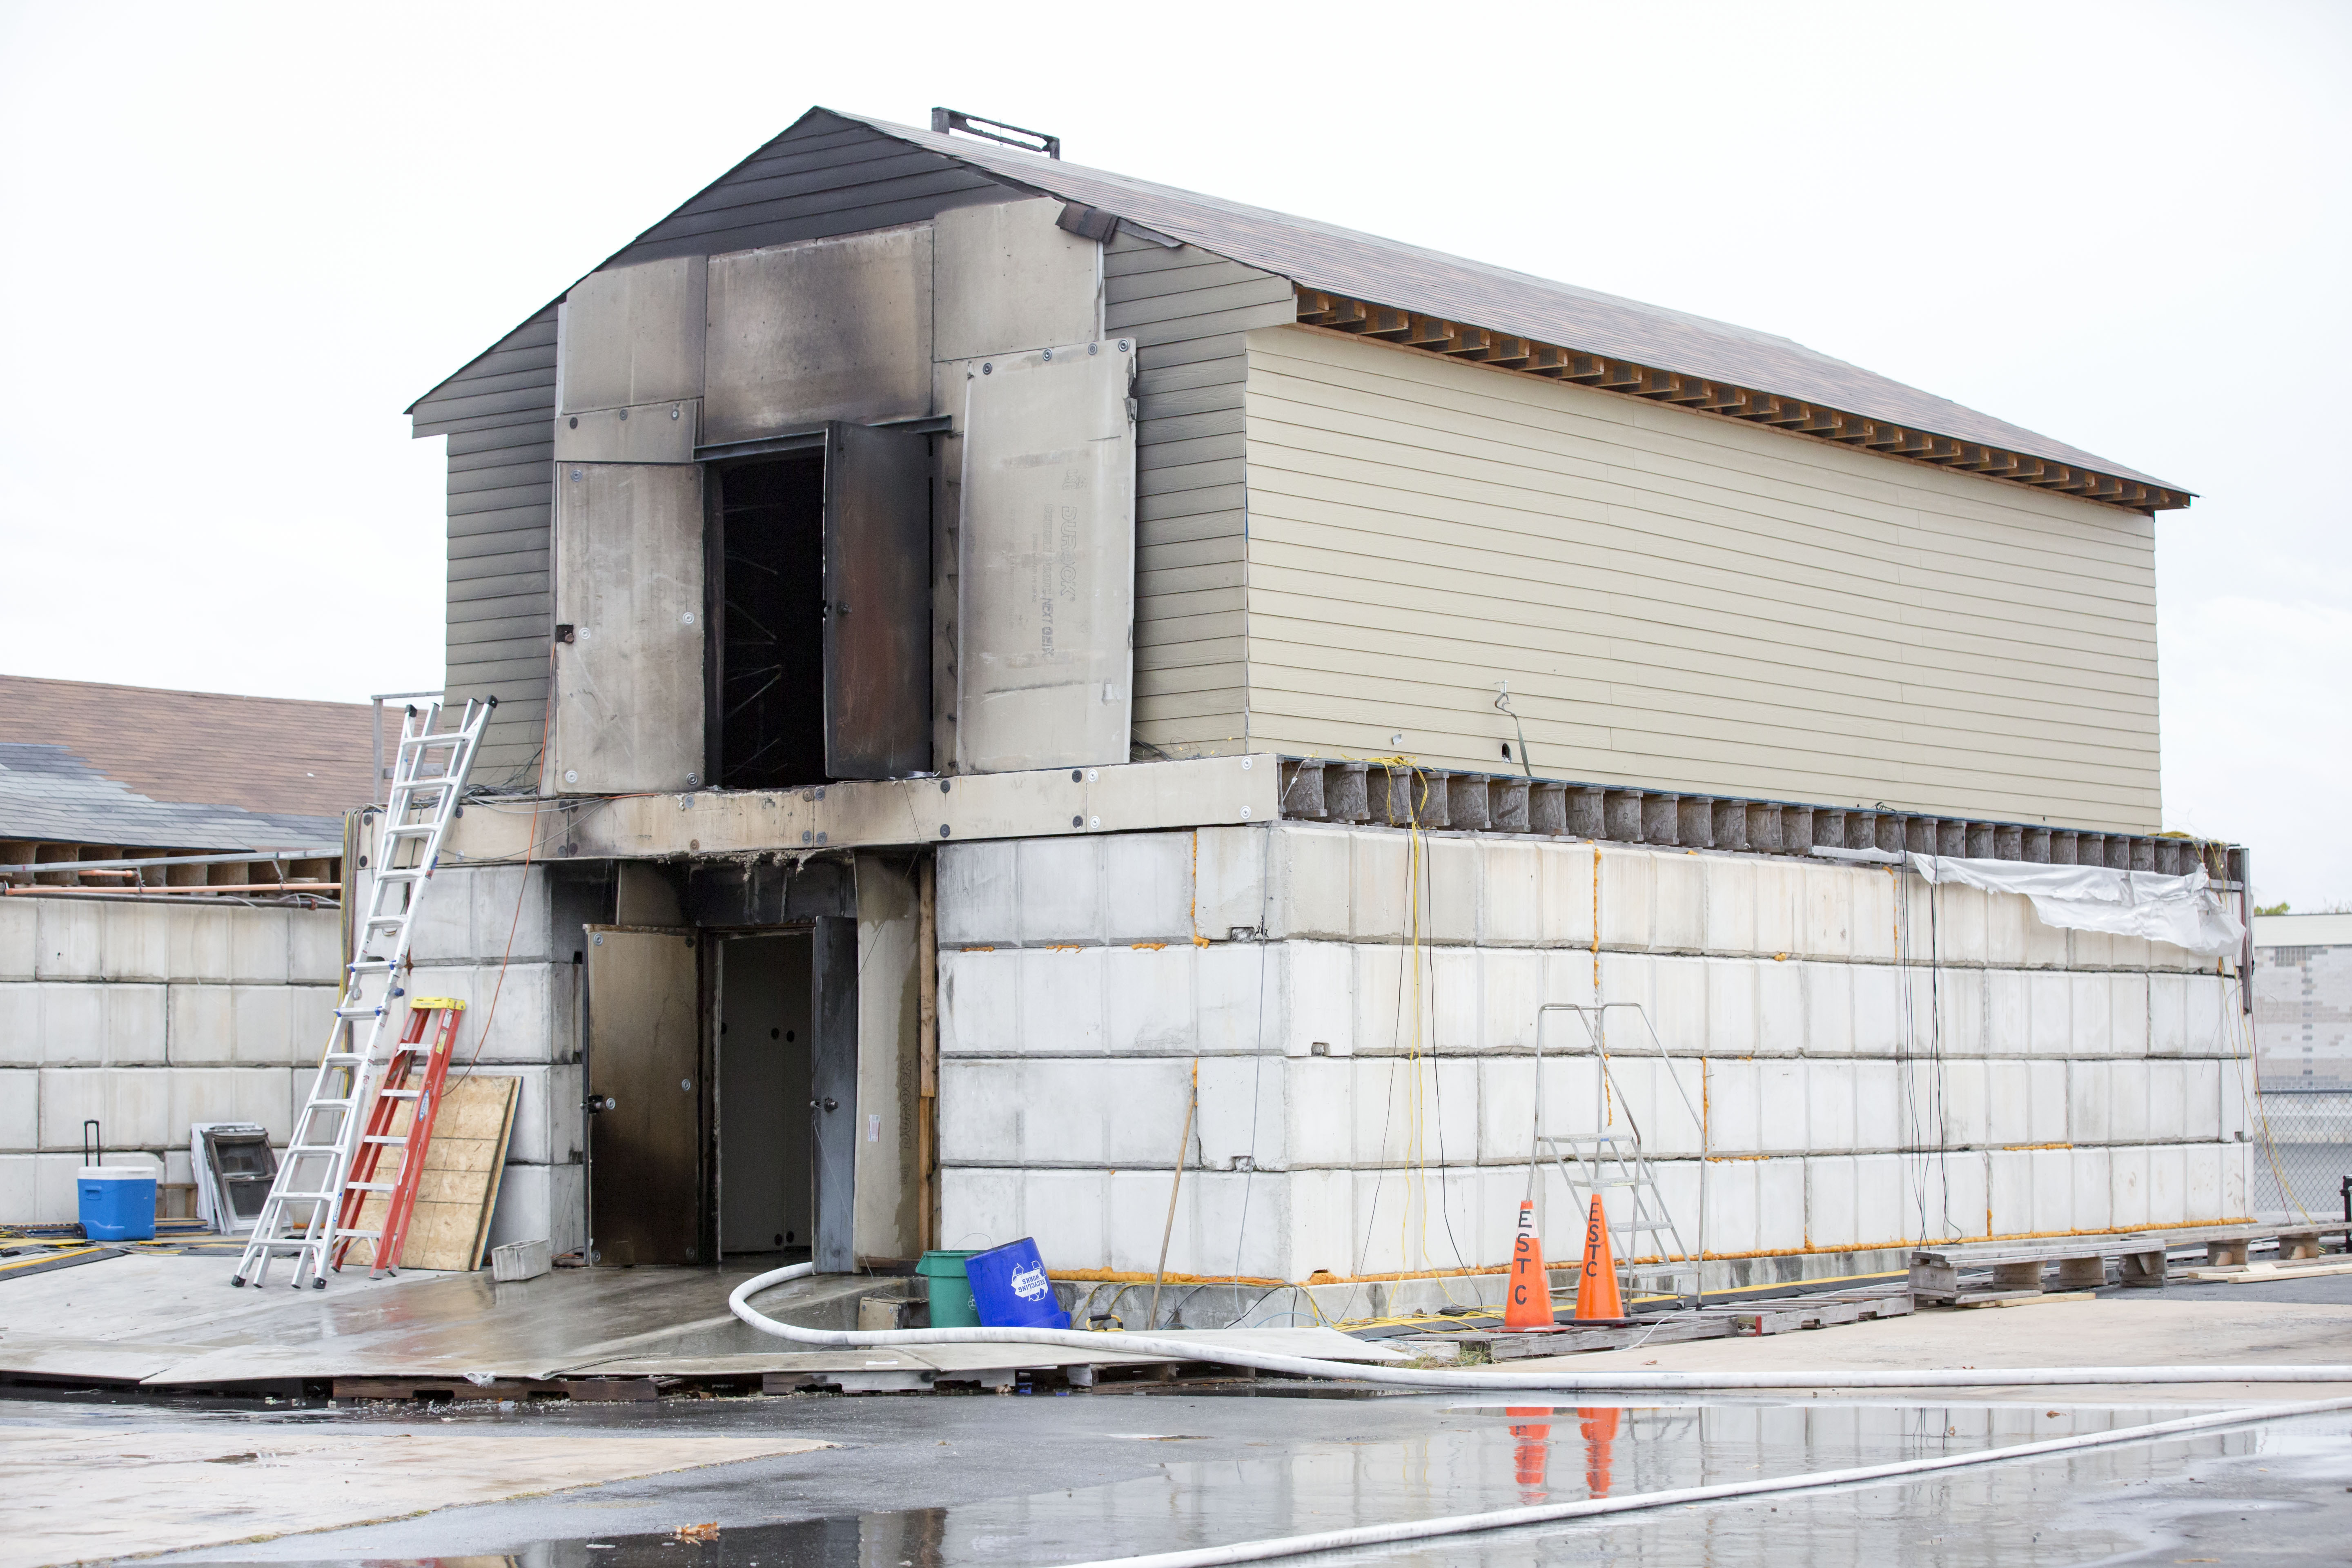
\includegraphics[width=6in]{Figures/Air_Entrainment/delcocorner.jpg}
	\caption{Delaware County, PA Fire Test Structure}
	\label{fig:Delaware_County,_PA_Fire_Test_Structure}
\end{figure}

The two-story concrete structure was built on a concrete slab as shown in Fig.~\ref{fig:Delaware_County,_PA_Fire_Test_Structure}. It was designed to simulate a representative residential structure. The outer wall of the structure was composed of interlocking concrete blocks 2~ft. wide, 2~ft. high, and 4~ft. long. The interior dimensions of the structure was 20~ft. wide, 36~ft. long, and 8~ft. high. The joints and gaps between the blocks were filled with high temperature insulation.

\clearpage

\begin{figure}[!ht]
	\centering
	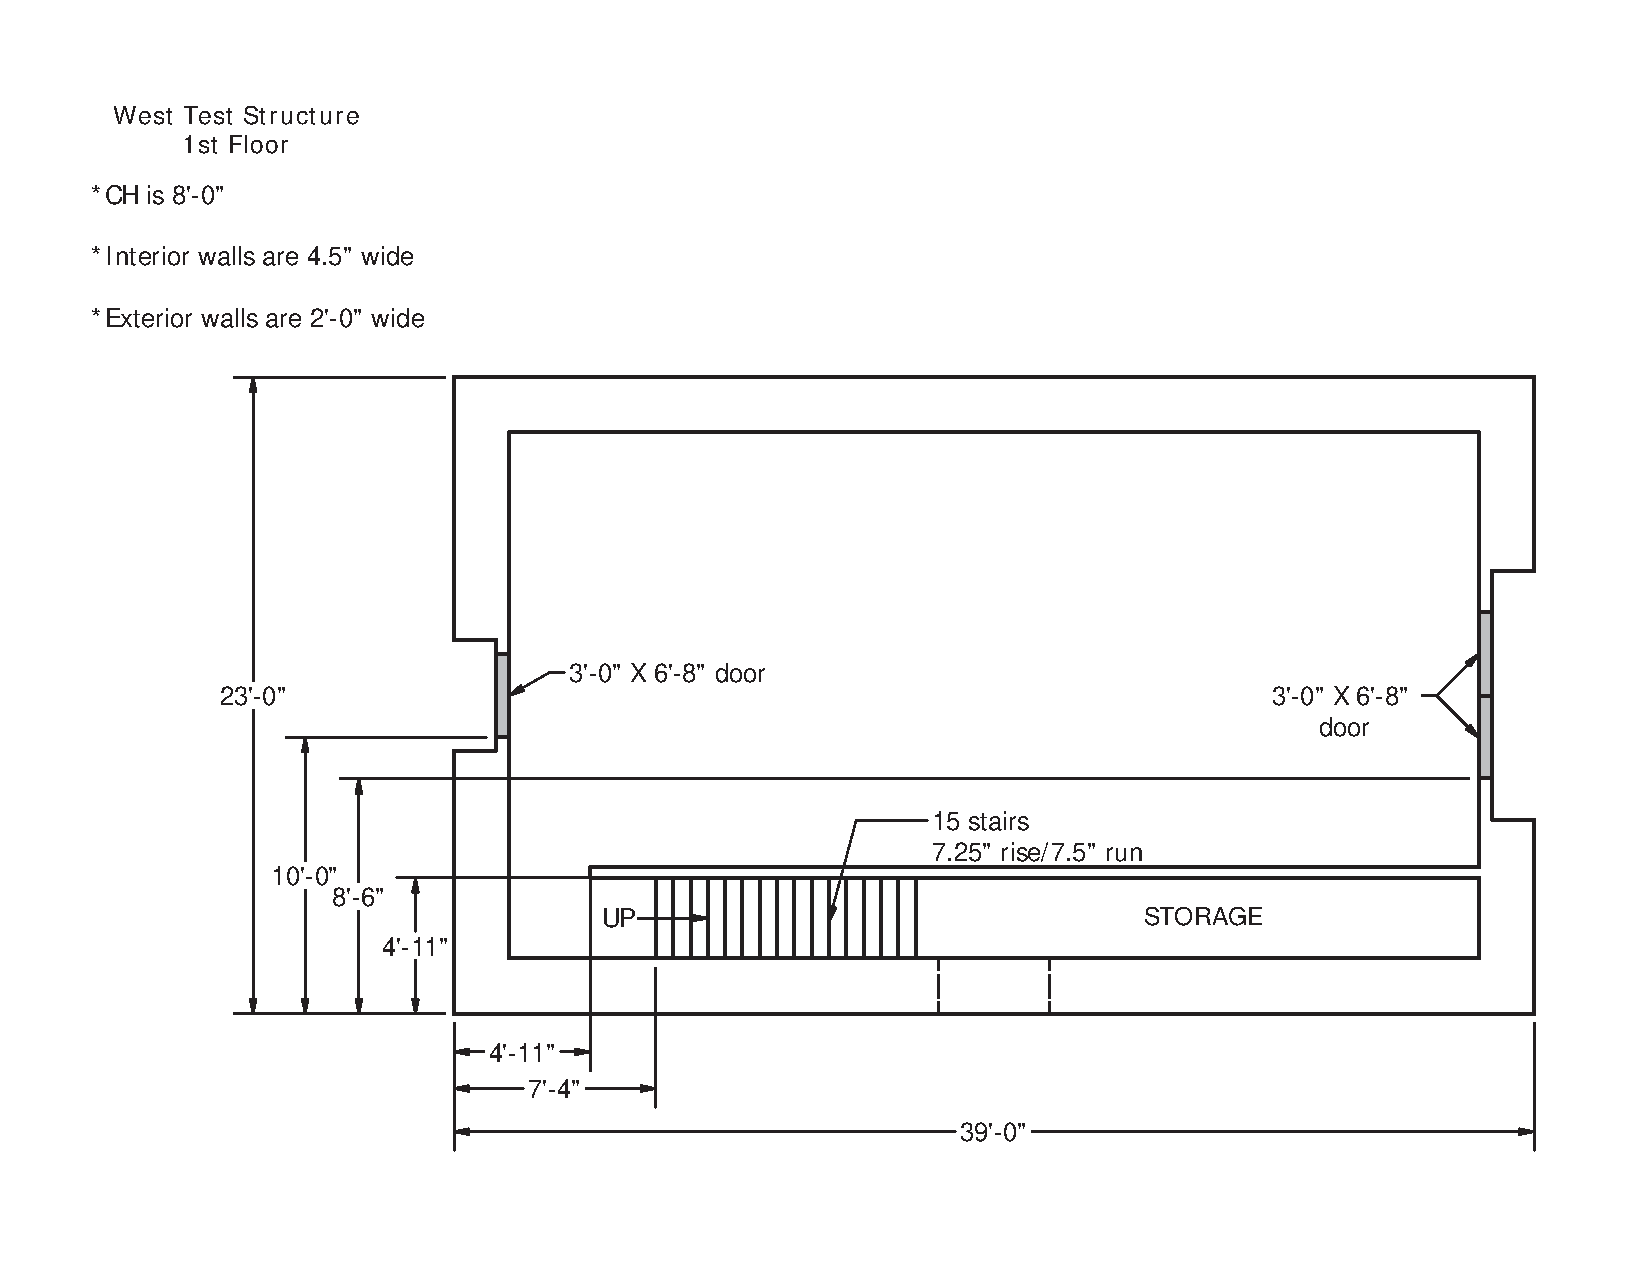
\includegraphics[width=5in]{Figures/Air_Entrainment/West_Test_Structure_1st_Floor_original_nodim.pdf}
	\caption{Delaware County, PA Fire Test Structure First Floor}
	\label{fig:Delaware_County,_PA_Fire_Test_Structure_First_Floor}
\end{figure}

\begin{figure}[!ht]
	\centering
	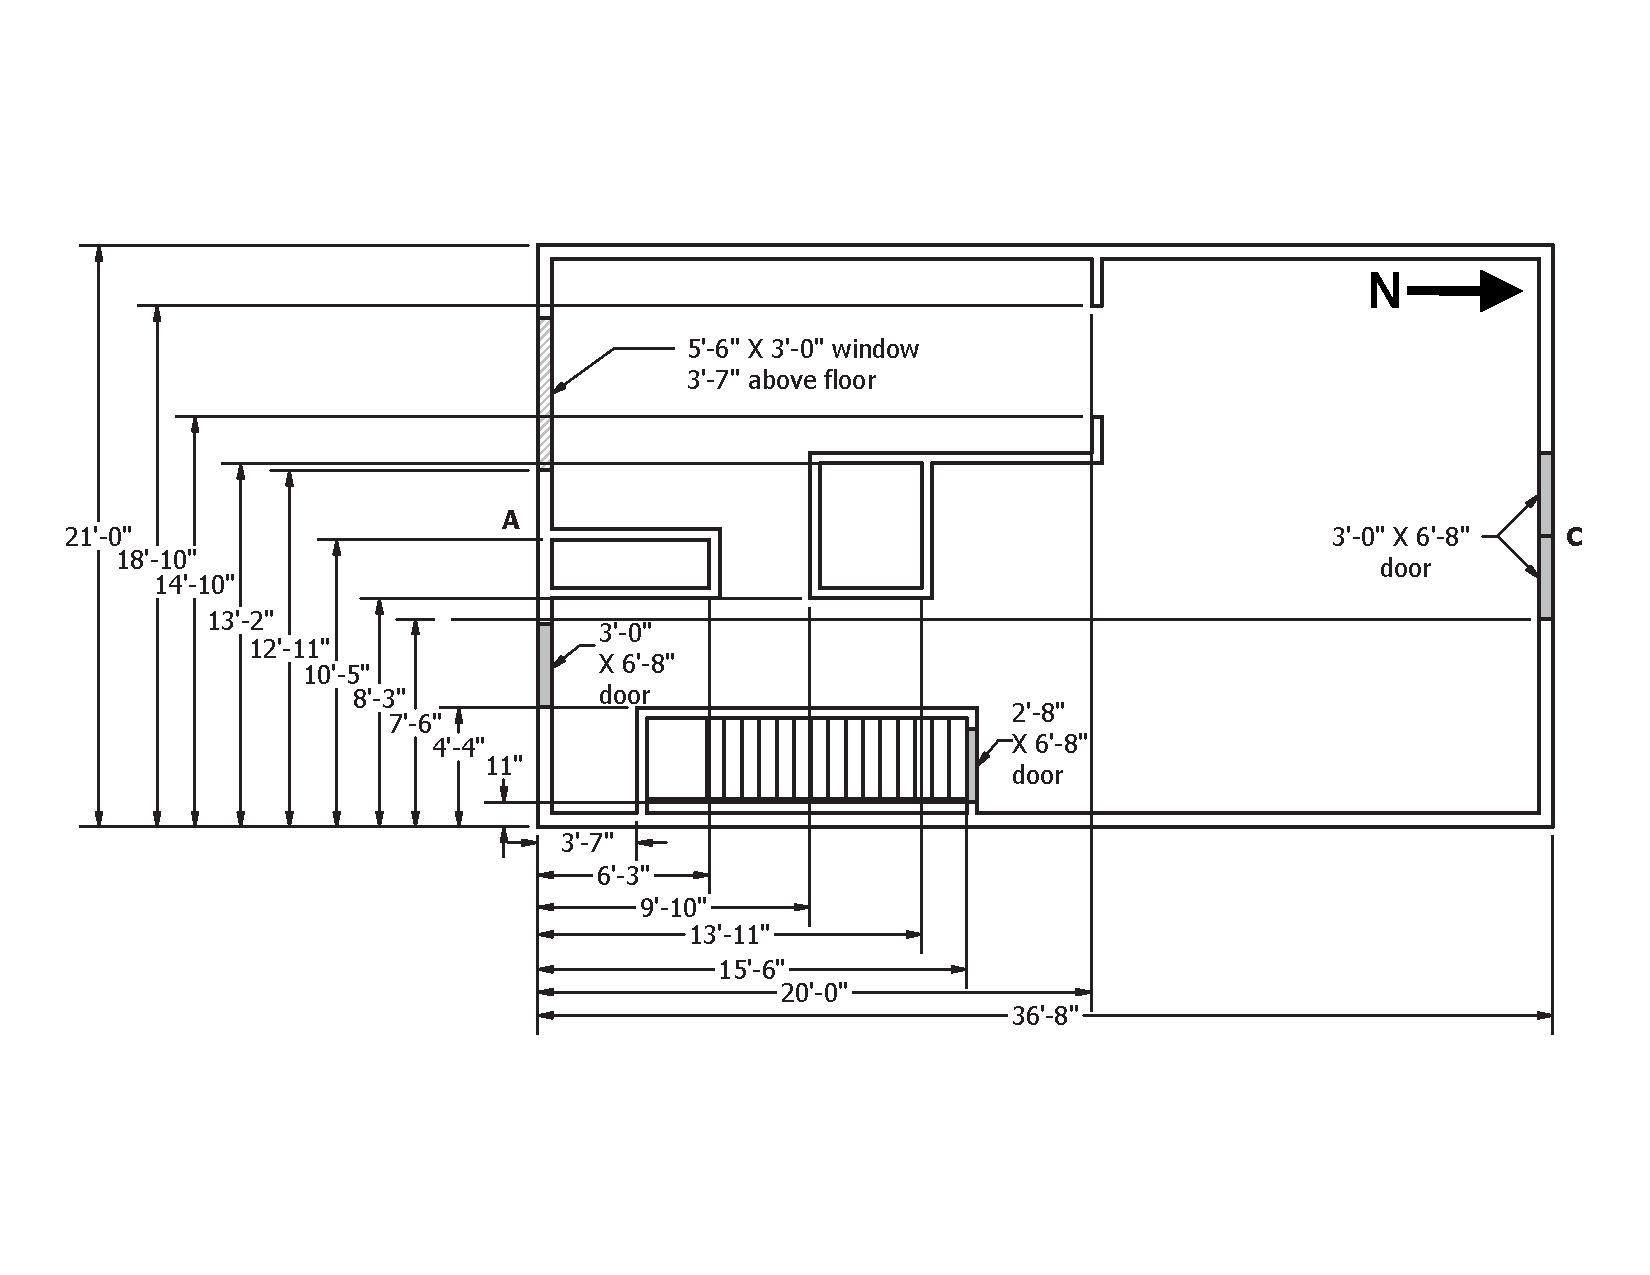
\includegraphics[width=5in]{Figures/Air_Entrainment/West_Test_Structure_2nd_Floor_nodim.pdf}
	\caption{Delaware County, PA Fire Test Structure Second Floor}
	\label{fig:Delaware_County,_PA_Fire_Test_Structure_Second_Floor}
\end{figure}

\clearpage

The interior walls of the first floor were framed with steel studs set to 16~in. centers and track and were lined with 0.5~in. thick cement board. The walls were composed of 0.6~in. Type X gypsum board. Additionally, the ceiling was composed of two layers of 0.5~in. thick cement board. The first floor ceiling support of the structure was composed of wood truss joist I-beams (TJIs) with a 11.75~in. depth. Each TJI was composed of laminated veneer lumber flanges with a cross section of 1.13~in. x 1.75~in. and an 0.43~in. thick oriented strand board web. Tongue and groove oriented strand board of 0.72~in. thickness was screwed to the top of the TJIs. The second floor of the two story structure was built on the wood ceiling support described above and was connected to the first floor by a stairwell. The walls of the second floor were wood frame with nominal 2~in. by 4~in. studs set to 16~in. centers. The interior walls were protected by 0.6~in. fire rated gypsum board, 0.6~in. durarock board, and a second layer of 0.6~in. fire rated gypsum board. The exterior walls were protected with 0.4~in. oriented strand board and 0.3~in. fiber cement lap siding.

The interior layout of the structure can be seen in the dimensioned floor plans above. The interior dimensions of the first and second floors of the structure were 19~ft. by 35.1~ft. and 20~ft. by 35.8~ft., respectively. The stairs connecting the two floors of the structure started 5.3~ft. off the South wall with a width of 4~ft. off the East wall and contained a 7.25~in. rise and 7.5~in. run. The exterior doorways of each structure and the stairwell doorway on the second level of the structure all contained steel doors that were opened or closed at certain instances during tests to change the ventilation configuration within the structure. All other doorways in the structures did not contain a door. If it was determined that these doors needed closed during a test, a sheet of either gypsum board or oriented strand board was used to cover the opening and remainded as such until the conclusion of the given test.

\subsubsection{Instrumentation}

% In order to obtain the results for Part I of this study, sensors were installed in the test fixtures to record measurements throughout the experiments. The instrumentation used varied between the air entrainment and the water distribution testing. The instrtuments, and associated uncertainty, used for each test series is outlined below.

To determine the amount of air entrained in hose streams, gas velocity was obtained through the use of an array of bi-directional probes in conjunction with differential pressure transducers and inconel thermocouples. The bi-directional probe was constructed of stainless steel and features a `high' side and a `low' side in which gases travel, through tubing, back to a pressure transducer that evaulates the differential pressure from ambient pressure. The iconel thermocouples were placed in-line wtih the bi-directional probes to ensure that the measurements were recorded at the same location. The iconel thermocouple was a 0.063~in. diameter type KSL iconel 600 sheathed grounded junction with a type K, 24~gauge glass/glass insulation lead. The differential pressure transducer was a Setra Model 264 with a range of +/- 0.5~in. WC (+/- 124.5~Pa.). The uncertainty given by the manufacturer is 1\% or 1.2~Pa. \hl{The configuration had a velocity range of +/- 24.2~m/s (+/- 54~mph).} The pressure transducers were configured in groups of six, contained in a single plastic box with connections for pressure, temperature, and power (Figure \ref{fig:Gas_Velocity_Measurements}a). Five probes were installed in openings where velocity measurements were taken, centered horizontally in the opening (Figure \ref{fig:Gas_Velocity_Measurements}b). The opening in which the bi-directional probes were placed is 2~ft. 8~in. by 6~ft. 8~in. The probes were placed in the center of the doorway horizontally and spaced evenly vertically. Velocity measurement with this configuration was determined to have an uncertainty of +/- 5\% \cite{BDPInPoolFires}.

\begin{figure} [H]
	\centering
	\begin{tabular}{c c}
		\subfloat[Pressure Transducer Box]{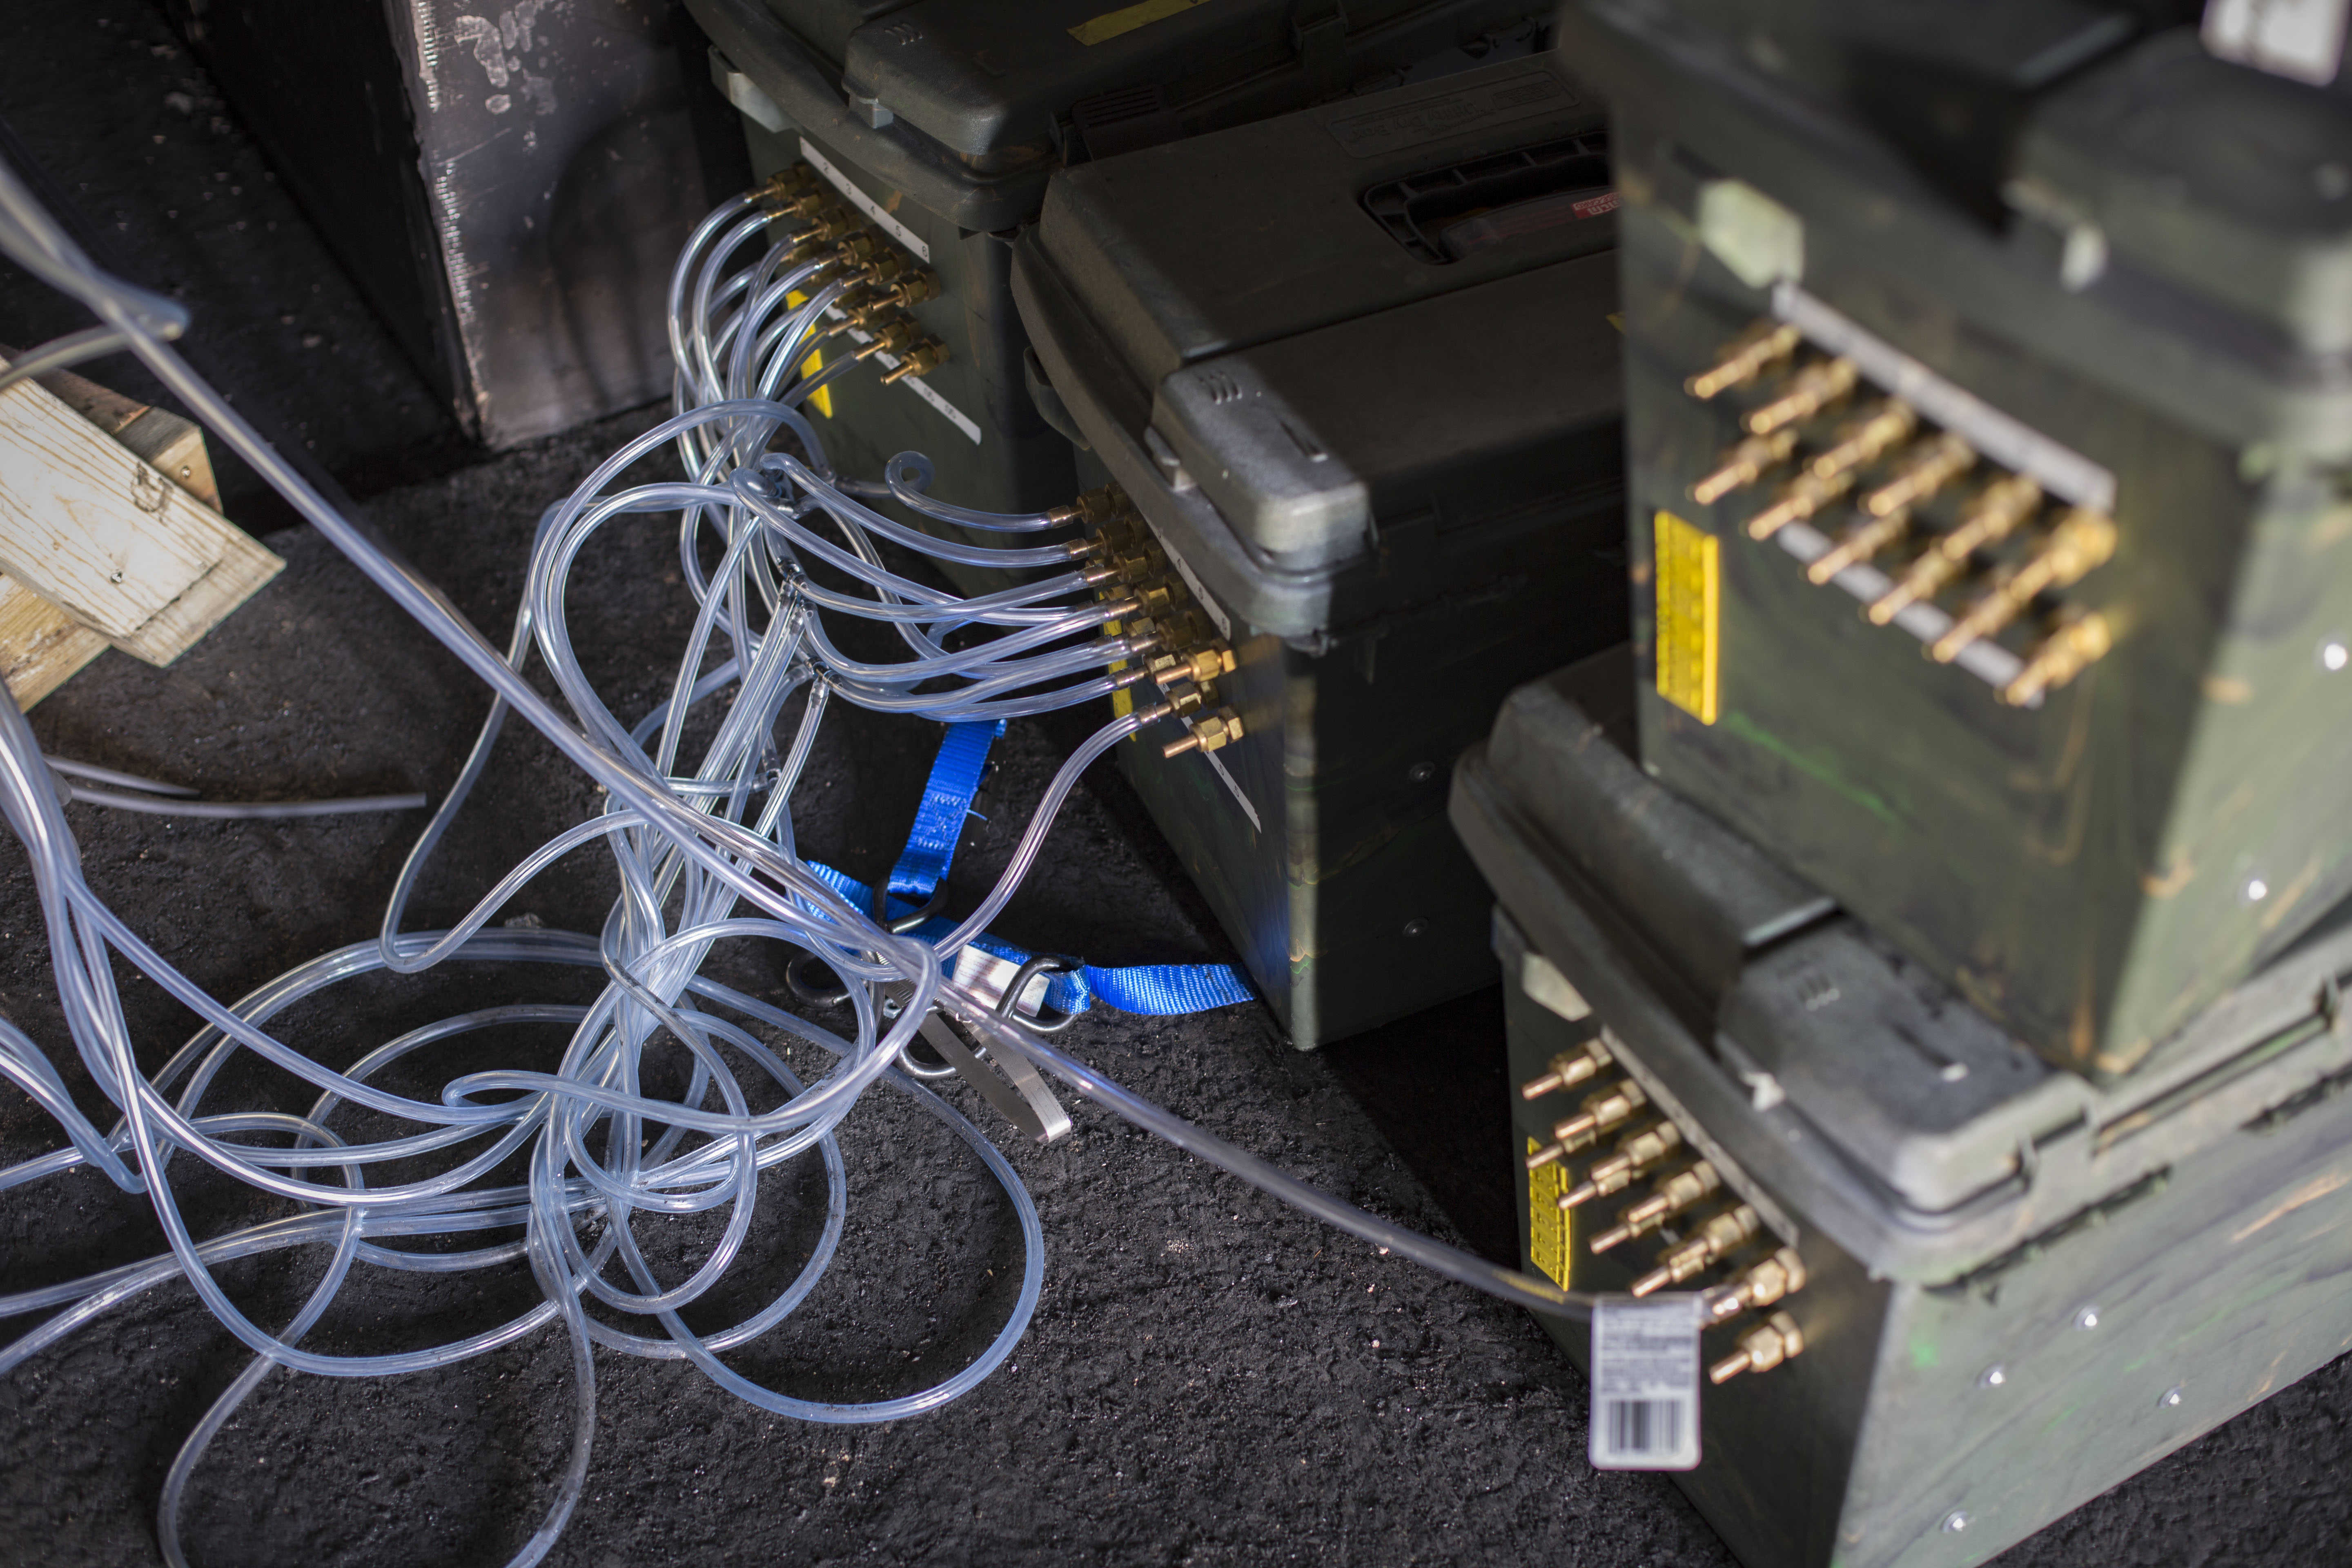
\includegraphics[height = 2.5in]{../0_Images/Instrumentation/BDPbox.jpg}} &
		\subfloat[Bi-Directional Probe Array]{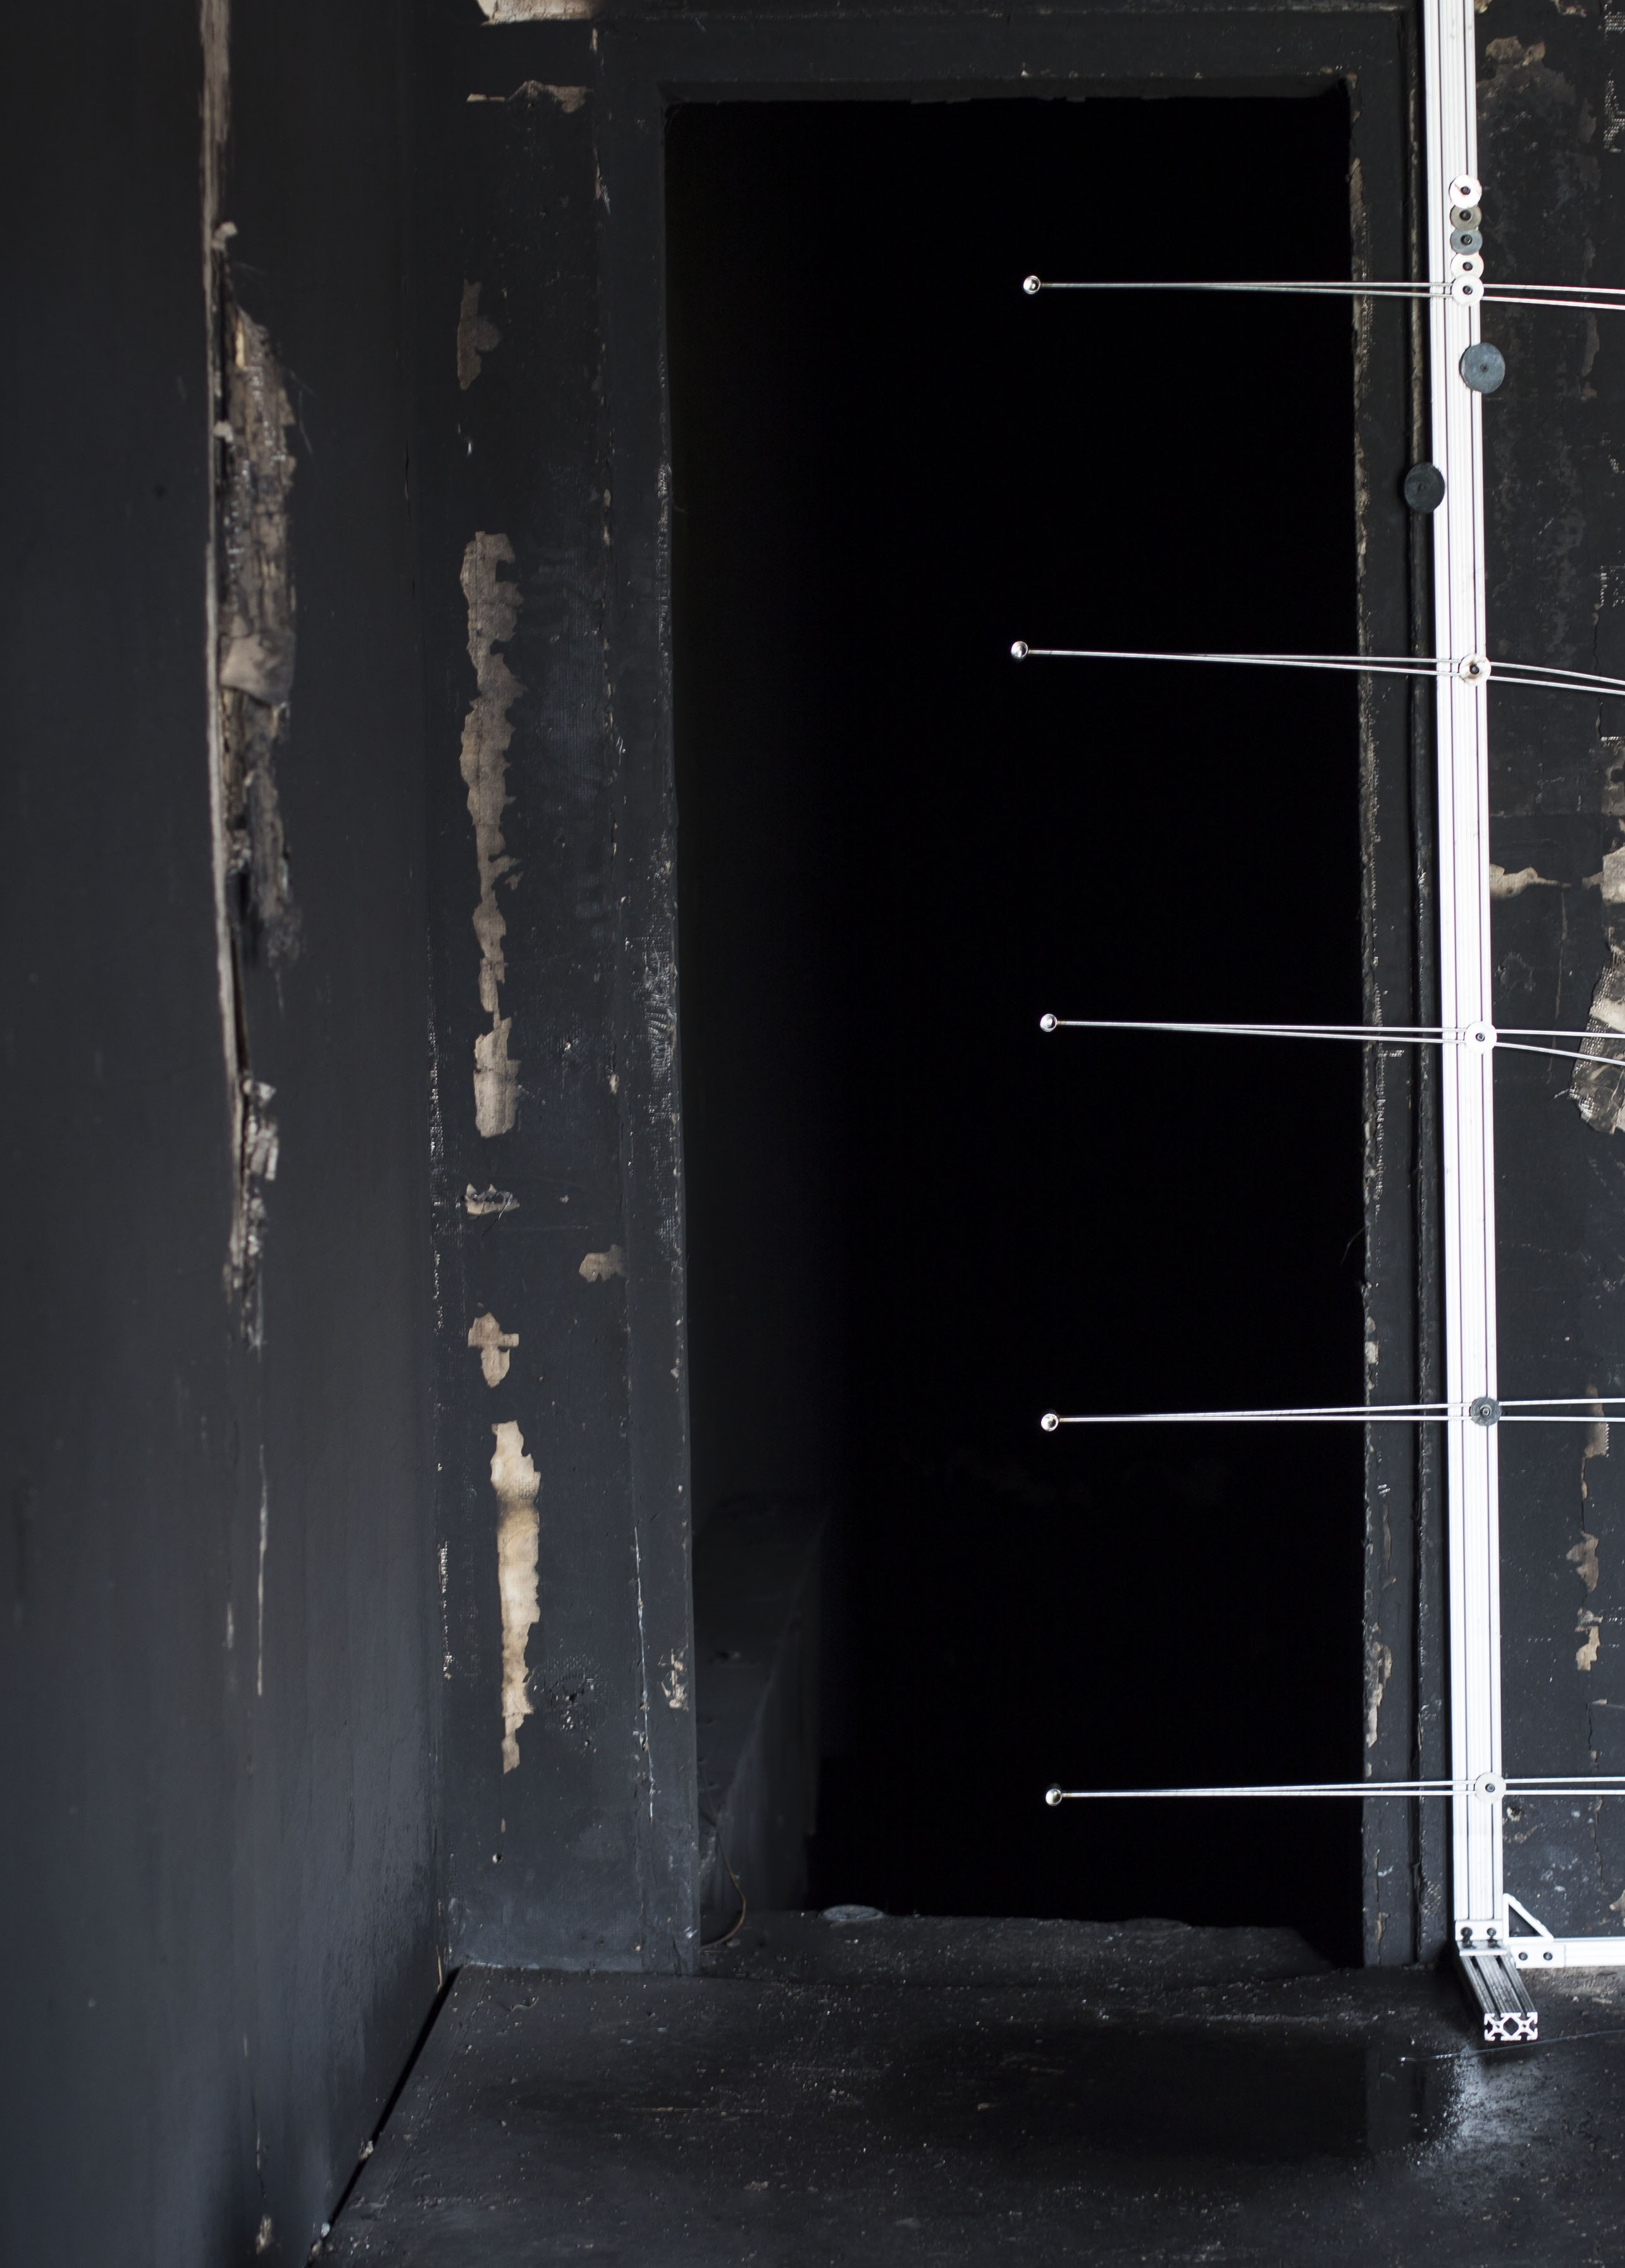
\includegraphics[height = 2.5in]{../0_Images/Instrumentation/BDParraydelco.jpg}} \\
	\end{tabular}
	\caption{Gas Velocity Measurements}
	\label{fig:Gas_Velocity_Measurements}
\end{figure}

% Standard video was obtained through the use of BoschVTC-206F03-4 video cameras (Figure \ref{fig:BullettCam}). All cameras were recorded via Samsung DVR.

% \begin{figure} [H]
% 	\centering
% 	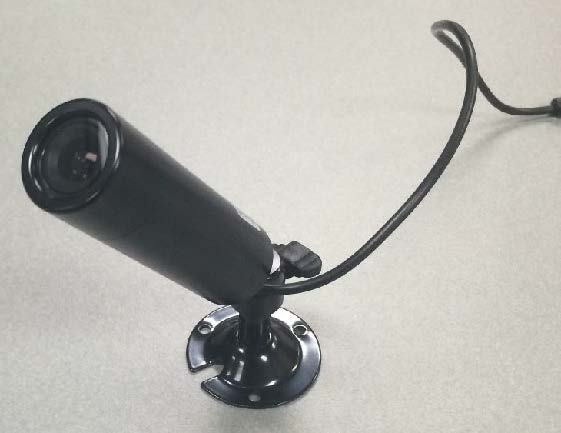
\includegraphics[width = 3in]{../0_Images/Instrumentation/BullettCam.jpg}
% 	\caption{Bullet Camera}
% 	\label{fig:BullettCam}
% \end{figure}

All data was logged through the use of a National Instruments data acquisition system incorporating a SCXI-1001 chassis with 8 SCXI-1102C 32-Channel modules (Figure \ref{fig:DataSystem}). The system is configured for a total of 256 channels capable of reading values between 0-10 volts DC. Values are recorded once a second and translated to quantities of interest through the use of LabVIEW software specifically programmed for use with the system.

\begin{figure}[H]
	\centering
	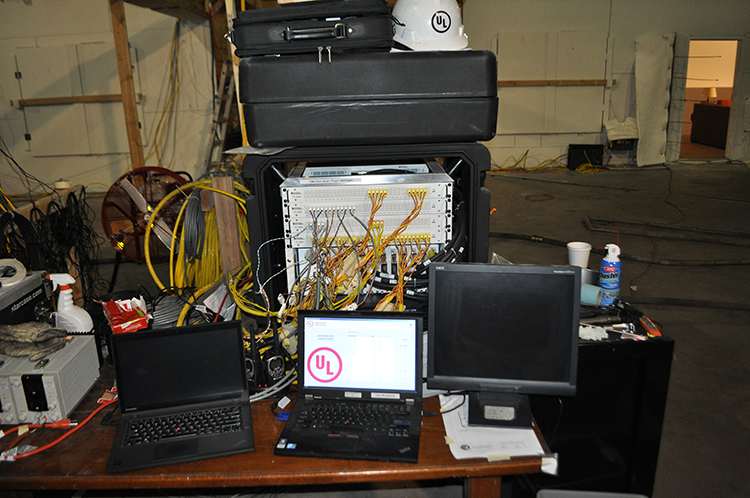
\includegraphics[width = 4in]{../0_Images/Instrumentation/DataSystem.jpg}
	\caption{Data Acquisition System}
	\label{fig:DataSystem}
\end{figure}

\clearpage

\subsubsection{Measurement Locations}

When examining the amount of air entrainment caused by variations in hose stream types, several challenges arose in determining the location to measure the gas velocity in the structure. Because the experiments were conducted in an outdoor fixture, considering environmental factors such as wind was critical; especially when quantifying the amount of air moved by hose streams. Additionally, the instrumentation used in data collection requires a dry environment to maintain the smallest level of uncertainty and remain operational. In order to combat these challenges, it was determined that the best way to acquire flow data would be to utilize the structure in such a way that there would be an inlet for replacement air, a measurement location, and an exhaust for both the hose streams and air moved. 

\begin{figure}[!ht]
	\centering
	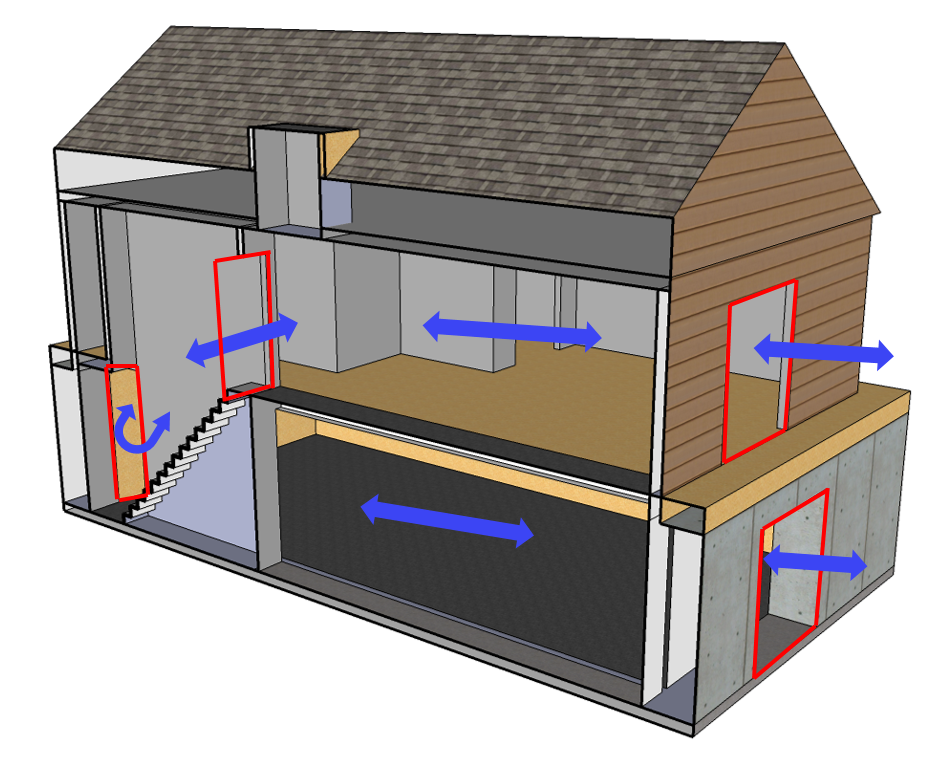
\includegraphics[width=3in]{Figures/Air_Entrainment/Airflow_flowpath}
	\caption{Air Entrainment Flowpath}
	\label{fig:Air_Entrainment_Flowpath}
\end{figure}

% \begin{figure}[!ht]
% 	\centering
% 	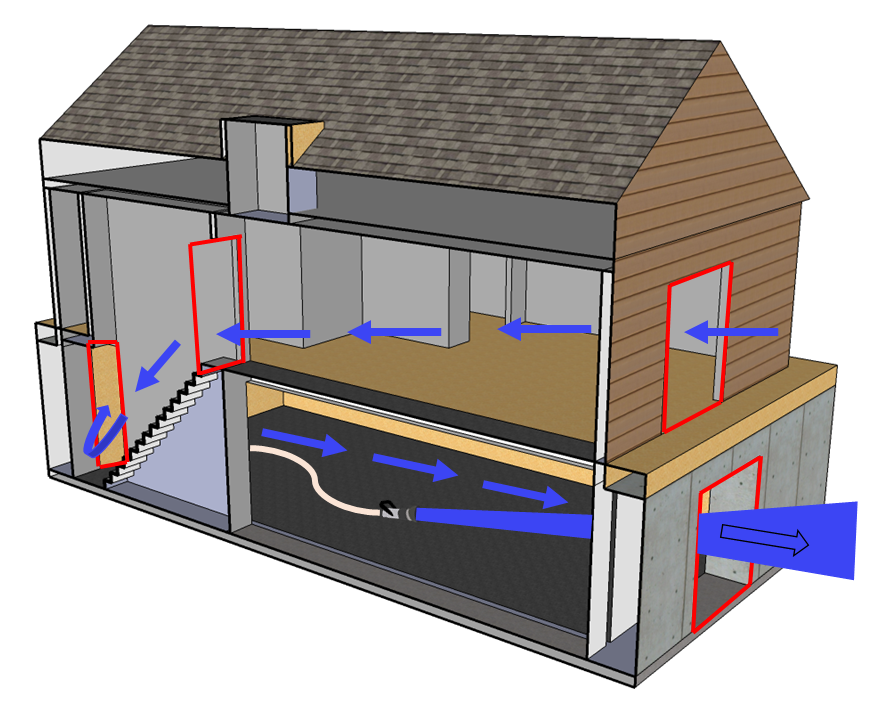
\includegraphics[width=5in]{Figures/Air_Entrainment/Airflow_Layout}
% 	\caption{Air Entrainment Flowpath, Interior Experiments}
% 	\label{fig:Air_Entrainment_Flowpath_Interior_Experiments}
% \end{figure}

% \begin{figure}[!ht]
% 	\centering
% 	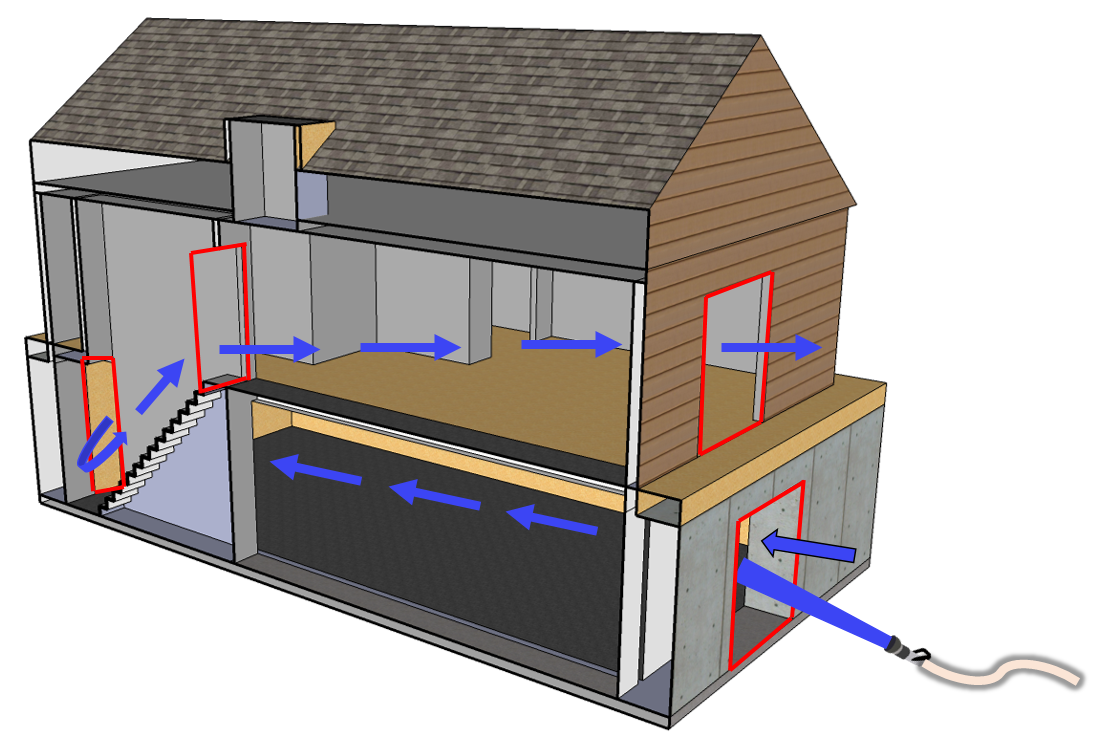
\includegraphics[width=4.5in]{Figures/Air_Entrainment/Airflow_Layout_Ext}
% 	\caption{Air Entrainment Flowpath, Exterior Experiments}
% 	\label{fig:Air_Entrainment_Flowpath_Exterior_Experiments}
% \end{figure}

% \clearpage

By placing the inlet and exhaust on the same side of the building, we can ensure that any presence of wind does not affect the pressure or air flow within the building. Therefore, the interior environment was consistent throughout the flow path as to not affect the measurements taken. The measurement location was placed in the inlet portion of the flow path in order to keep the instrumentation dry and out of the reach of a hose stream. With the exception of the predetermined inlet and outlet, the remainder of the ventilation openings in the structure remained closed throughout the duration of testing. This ensures that the air entrained by the nozzle is drawn from the inlet location and passes through the measurement location seen in Figure \ref{fig:Measurement_Location_Second_Floor}.

\begin{figure}[!ht]
	\centering
	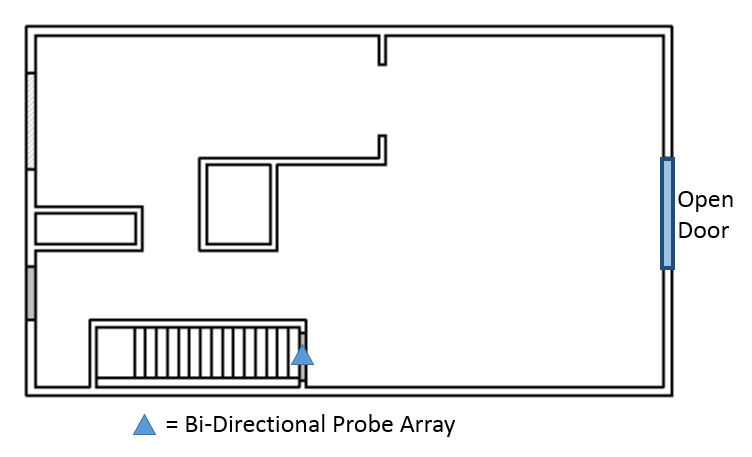
\includegraphics[width=3in]{Figures/Air_Entrainment/Measurement_Locations_Secondfloor}
	\caption{Measurement Location (Second Floor)}
	\label{fig:Measurement_Location_Second_Floor}
\end{figure}

\clearpage

\subsubsection{Equipment Used}

In order to ensure the data collected and associated results were applicable to the majority of the fire servce, our technical panel was tasked with creating a list of represetative nozzles, specified flow rates/pressures, and nozzle movement techniques. All of these variables were tested during the air entrainment experiments; however, several other aspects were held constant such as the length of hose used. The nozzles utilized during these experiments can be seen in the table below.

\vspace*{\baselineskip}

\begin{table}[!ht]
\centering
\begin{tabular}{|llccc|}
\hline
\multicolumn{1}{|l|}{\textbf{Line Size}} & \multicolumn{1}{l|}{\textbf{Nozzle}} & \multicolumn{1}{l|}{\textbf{Tip (in)}} & \multicolumn{1}{l|}{\textbf{Nozzle Pressure (psi)}} & \textbf{Approximate Flow Rate (gpm)} \\ \hline
1 3/4 in. & Smooth Bore & 1 & 50 & 210 \\
 & Smooth Bore & 15/16 & 50 & 180 \\
 & Smooth Bore & 7/8 & 50 & 150 \\
 & Fog &  & 100 & 100 \\
 & Fog &  & 100 & 150 \\
 & Fog &  & 75 & 150 \\
 & Fog &  & 50 & 150 \\ \hline
2 1/2 in. & Smooth Bore & 1 1/8 & 50 & 260 \\
 & Smooth Bore & 1 1/4 & 50 & 320 \\
 & Fog &  & 100 & 250 \\
 & Fog &  & 75 & 250 \\
 & Fog &  & 50 & 250 \\ \hline
Portable Monitor & Smooth Bore & 1 3/8 & 80 & 500 \\
 & Fog &  & 75 & 500 \\ \hline
Master Stream & Smooth Bore & 1 1/2 & 80 & 600 \\
 & Smooth Bore & 1 3/4 & 80 & 800 \\
 & Fog &  & 100 & 500-1000 \\ \hline
\end{tabular}
\caption{Nozzle Selection}
\label{Nozzle Selection}
\end{table}

\vspace*{\baselineskip}

When determining how to create a test setup that would involve the repetition of nozzle movements and patterns, it was vital to ensure human fatigue of the nozzle operator would not affect the results. Thus, the UL - FSRI engineers designed a nozzle prop to serve as the `backup' firefighter by supporting the hoseline and nearly eliminating any potential nozzle reaction and fatigue. 

\begin{figure}[!ht]
\centering
	\includegraphics[width=3in]{Figures/Air_Entrainment/hoserig.jpg}
	\caption{Nozzle Prop}
	\label{fig:Nozzle_Prop}
\end{figure}

\clearpage

The hose was affixed to the prop with `C' clamps and locking nuts to ensure the hose did not move during a given experiment. The prop served as support for both 1.5~in. and 2.5~in. hoseline sizes. The distance from the nozzle to the ventilation opening was measured from the tip of the nozzle, and not the base of the prop, and thus the measurements between the experiments were consistent.

\vspace*{\baselineskip}

\begin{figure}[!ht]
\centering
\begin{tabular*}{\textwidth}{cc}
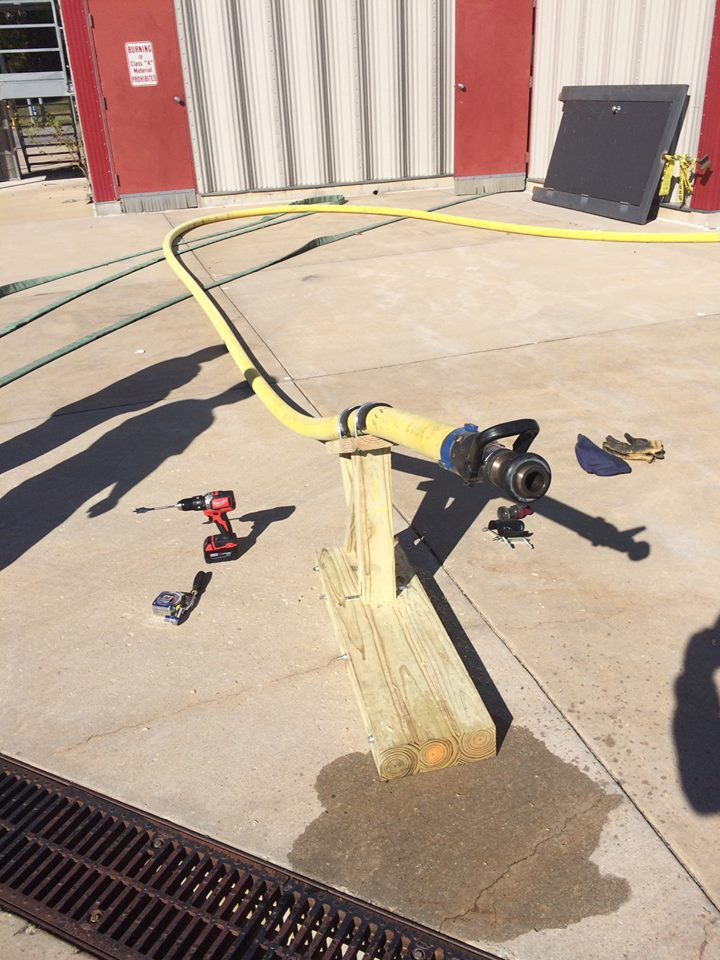
\includegraphics[width=2.5in]{Figures/Air_Entrainment/Old_Gib.jpg} &
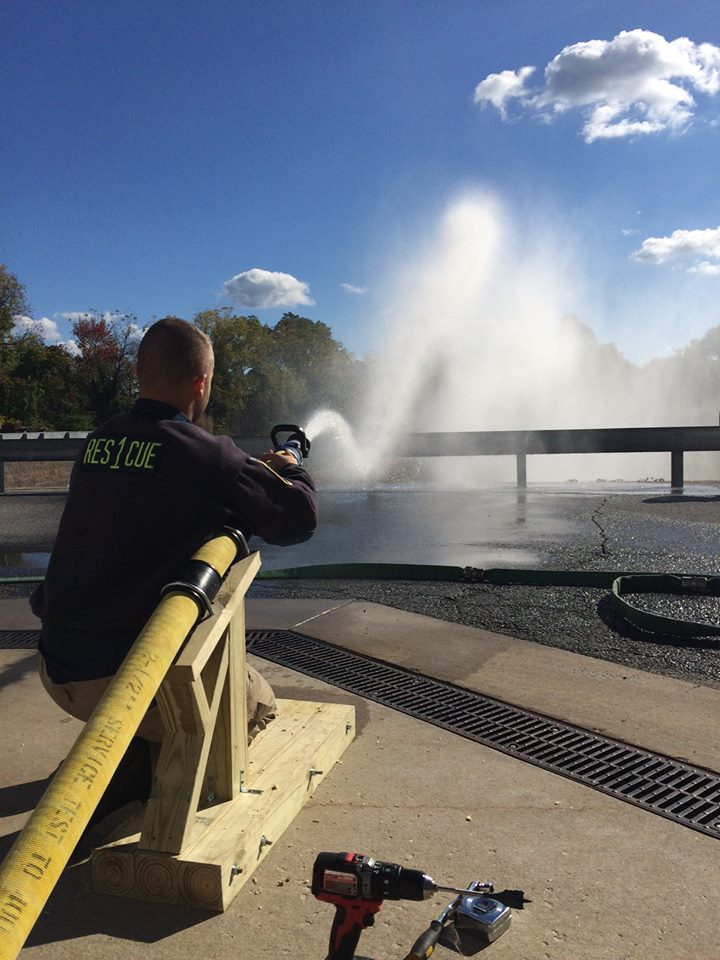
\includegraphics[width=2.5in]{Figures/Air_Entrainment/Old_Gib_1.jpg} \\
\end{tabular*}
\caption{Nozzle Prop in Use}
\label{fig:Nozzle_Prop_in_Use}
\end{figure}

\clearpage

\subsection{Experiments Conducted}

The experiments to determine the amount of air entrained by hose streams consisted of several test series to gain a wholelistic view of how varying different components, either with the structure or equipment utilized, affected the end result.

Prior to determining the parameters for the test series' below, several preliminary experiments were conducted in order to provide insight into several key components including the setback distance from the nozzle to the ventilation opening, the hose stream type, and various nozzle movements.

\begin{itemize}

\item \bf{Setback Distance}
\normalfont
\vspace*{\baselineskip}

Two experiments were conducted on the interior of the structure utilizing a 1.5~in. combination nozzle with a flow rate of 150~gpm to determine the effects of altering the setback distance of the nozzle to the ventilation opening on the overall air entrainment in the hose stream. The first of the two tests examined setback distances of 3, 6, 9, 12, and 15~feet from the open double door at a pressure of 50~psi. The second test examined the same setback distances at a nozzle pressure of 100~psi.  

\vspace*{\baselineskip}

\item \bf{Hose Stream Type}
\normalfont
\vspace*{\baselineskip}

To gain an initial look into the hose stream type, a fixed setback distance of 3~ft. was chosen and the nozzle was varied to a wide fog pattern (nearly occluding the ventilation opening), a narrow fog pattern (roughly 30~deg.), and a straight stream pattern. This provided preliminary information that aided in the test setup for the remainder of the experiments. The nozzle used during this test was a 1.5~in. combination nozzle with a flow rate of 150~gpm and a pressure of 100~psi.

\vspace*{\baselineskip}

\item \bf{Nozzle Movements}
\normalfont
\vspace*{\baselineskip}

Because there are numerous nozzle movements that firefighters can employ during suppression operations, it was vital that the UL - FSRI team identify any differences in air entrainment prior to conducting the remainder of the study. This would provide information into whether or not the various nozzle movements would all be tested or if some could be eliminated due to similarities in results. These tests were conducted with a fixed setback distance of 18~ft. from the ventilation opening and utilized both a 1.5~in. combination nozzle with a flow rate of 150~gpm and a pressure of 100~psi and a 1.5" smooth bore nozzle with a 1" tip flowing 210~gpm at a pressure of 50~psi.

\vspace*{\baselineskip}

\item \bf{Manufacturer Comparison}
\normalfont
\vspace*{\baselineskip}

Similar to the issue above with various nozzle movements, fire departments across the world used nozzles made from different manufacturers. To provide some insight into the accuracy of manufacturer ratings of flow rate and pressure in addition to air entrainment, several experiments were conducted to determine the differences in nozzle manufacturers. These experiments were all conducted with both a 1.5~in. combination nozzle and a 1.5~in. smooth bore nozzle. This would provide information into the differences in air entrainment between nozzles with similar flow rates and pressures made by different manufacturers.

\vspace*{\baselineskip}

\end{itemize}

\clearpage

\subsubsection{Total Air Entrainment Comparison}

The first test series of the air entrainment experiments looked at the differences in total entrainment given a single nozzle manufacturer with varying flow rates and pressures. These tests were conducted from both the interior and exterior of the structure at a setback distance of 18~ft. from the ventilation opening. 

An `Event' is defined as a specific measurement period during the experiment in which a specific variable is being analyzed. For example, during the total air entrainment experiment for 1.5~in. combination nozzles from the interior, 6 different events were incorporated within the test: 1) Straight Stream, 2) Straight Stream `O', Straight Stream `Z', Straight Stream `n', Narrow Fog, and Narrow Fog `O'. In order to ensure consistency among results, each of the `Events' within the experiments was designed to be 1 minute in duration. 

\begin{figure}[!ht]
	\centering
	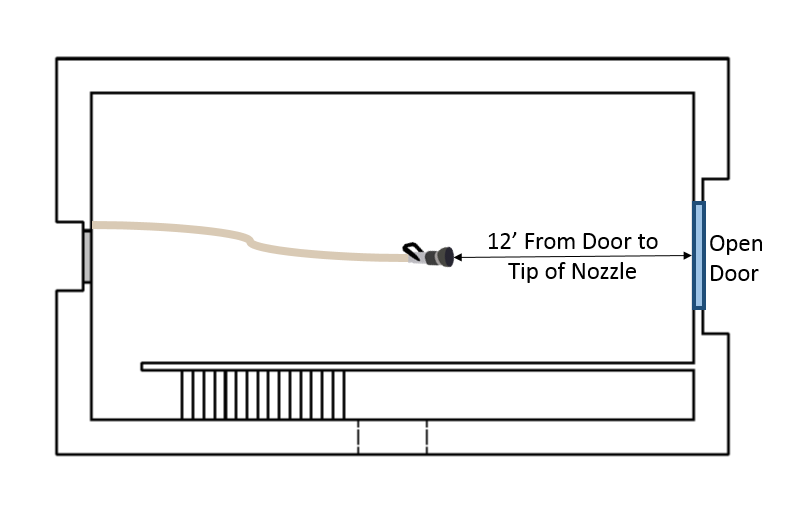
\includegraphics[width=4in]{Figures/Air_Entrainment/Measurement_Locations_Firstfloor}
	\caption{First Floor Setup - Total Entrainment Interior Tests}
	\label{fig:First_Floor_Setup_Total_Entrainment_Interior_Tests}
\end{figure}

\begin{figure}[!ht]
	\centering
	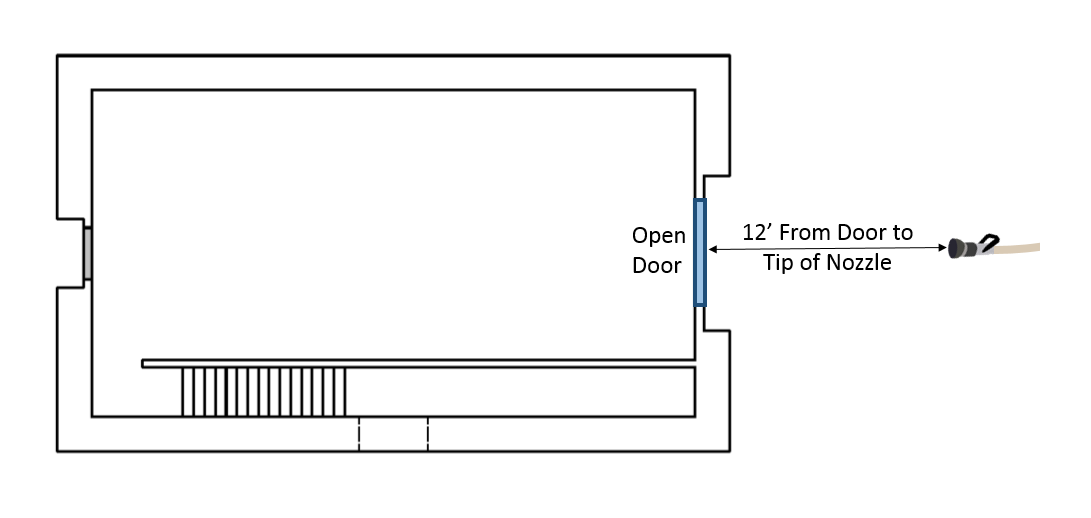
\includegraphics[width=6.5in]{Figures/Air_Entrainment/Measurement_Locations_Firstfloor_Ext}
	\caption{First Floor Setup - Total Entrainment Exterior Tests}
	\label{fig:First_Floor_Setup_Total_Entrainment_Exterior_Tests}
\end{figure}

\clearpage

\begin{figure}[!ht]
	\centering
	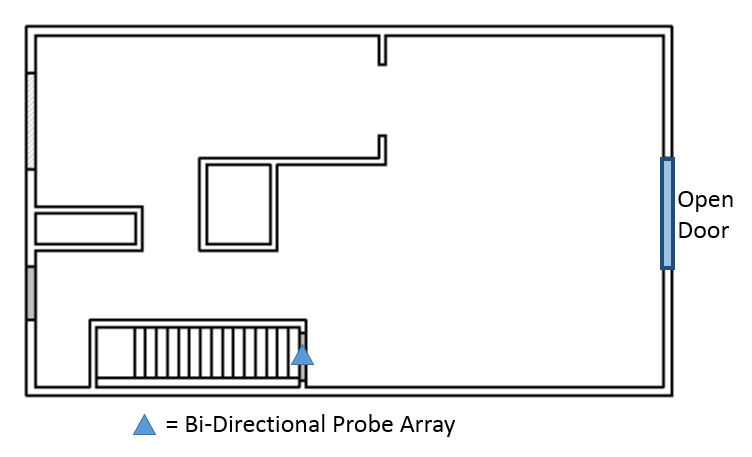
\includegraphics[width=4in]{Figures/Air_Entrainment/Measurement_Locations_Secondfloor}
	\caption{Second Floor Measurement Location}
	\label{fig:Second_Floor_Measurement_Location}
\end{figure}

\vspace*{\baselineskip}

\begin{table}[!ht]
\centering
\begin{tabular}{|lcclccc|}
\hline
\multicolumn{1}{|c|}{\textbf{Location}} & \multicolumn{1}{c|}{\textbf{Nozzle Size}} & \multicolumn{1}{c|}{\textbf{Manufacturer}} & \multicolumn{1}{c|}{\textbf{Nozzle Type}} & \multicolumn{1}{c|}{\textbf{Tip Size}} & \multicolumn{1}{c|}{\textbf{Flow Rate}} & \textbf{Pressure} \\ \hline
Interior & 1.5 & MF1 & Combination &  & 95 & 100 \\
Interior & 1.5 & MF1 & Combination &  & 150 & 50 \\
Interior & 1.5 & MF1 & Combination &  & 150 & 75 \\
Interior & 1.5 & MF1 & Combination &  & 150 & 100 \\
Interior & 1.5 & MF1 & Smooth Bore & 7/8 & 150 & 50 \\
Interior & 1.5 & MF1 & Smooth Bore & 15/16 & 180 & 50 \\
Interior & 1.5 & MF1 & Smooth Bore & 1 & 210 & 50 \\
Interior & 2.5 & MF1 & Combination &  & 250 & 50 \\
Interior & 2.5 & MF1 & Combination &  & 250 & 75 \\
Interior & 2.5 & MF1 & Combination &  & 250 & 100 \\
Interior & 2.5 & MF1 & Smooth Bore & 1 1/8 & 260 & 50 \\
Interior & 2.5 & MF1 & Smooth Bore & 1 1/4 & 320 & 50 \\
Interior & MS & MF1 & Combination &  & 500 & 100 \\
Interior & MS & MF1 & Combination &  & 750 & 100 \\
Interior & MS & MF1 & Smooth Bore & 1 1/2 & 600 & 80 \\
Interior & MS & MF1 & Smooth Bore & 1 3/4 & 800 & 80 \\
Interior & PM & MF1 & Combination &  & 500 & 80 \\
Interior & PM & MF1 & Smooth Bore & 1 3/8 & 480 & 80 \\
Exterior & 1.5 & MF1 & Combination &  & 150 & 75 \\
Exterior & 1.5 & MF1 & Smooth Bore & 15/16 & 180 & 50 \\
Exterior & 2.5 & MF1 & Combination &  & 250 & 75 \\
Exterior & 2.5 & MF1 & Smooth Bore & 1 1/4 & 320 & 50 \\
Exterior & PM & MF1 & Combination &  & 500 & 75 \\
Exterior & PM & MF1 & Smooth Bore & 1 3/8 & 500 & 80 \\ \hline
\end{tabular}
\caption{Total Air Entrainment Experiments}
\label{Total_Air_Entrainment_Experiments}
\end{table}

\clearpage

\subsubsection{Ventilation Configuration}

The second series of tests conducted to analyze air entrainment in hose streams involved varying the ventilation configurations within the flow path. The inlet and exhaust of the flow path were varied between both different sized doors as well as windows to show the effect on overall air entrainment. The tests were conducted from both the interior and the exterior of the structure with a fixed setback distance of 18~ft. from the ventilation opening. The measurement location during these experiments remained the same as that used during the total air entrainment experiments with the instrumentation remaining in the doorway at the top of the stairs on the second floor. (Figure \ref{fig:Second_Floor_Ventilation_Config})

\begin{figure}[!ht]
	\centering
	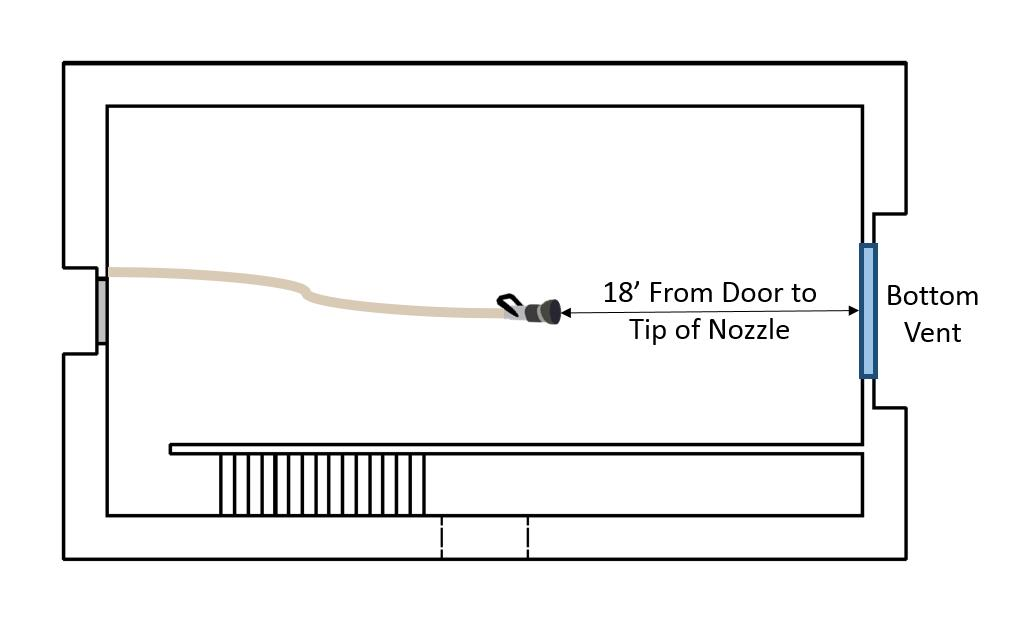
\includegraphics[width=5in]{Figures/Air_Entrainment/Measurement_Location_VentConfig_Bottom.jpg}
	\caption{First Floor Ventilation Configuration Interior}
	\label{fig:First_Floor_Ventilation_Configuration_Interior}
\end{figure}

\begin{figure}[!ht]
	\centering
	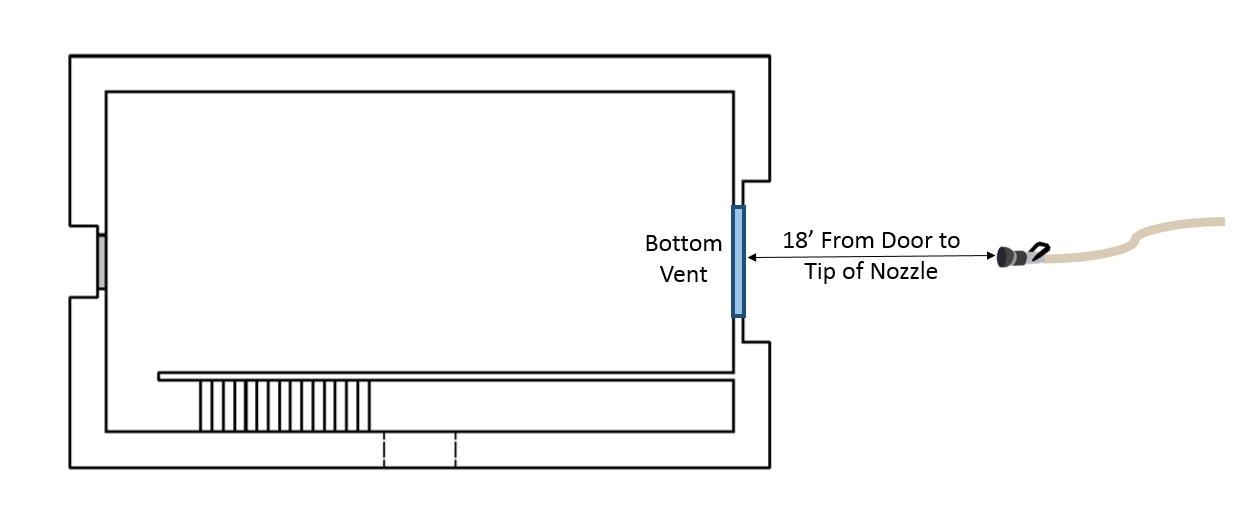
\includegraphics[width=6.5in]{Figures/Air_Entrainment/Measurement_Location_VentConfig_Bottom_Ext.jpg}
	\caption{First Floor Ventilation Configuration Exterior}
	\label{fig:First_Floor_Ventilation_Configuration_Exterior}
\end{figure}

\clearpage

\begin{figure}[!ht]
	\centering
	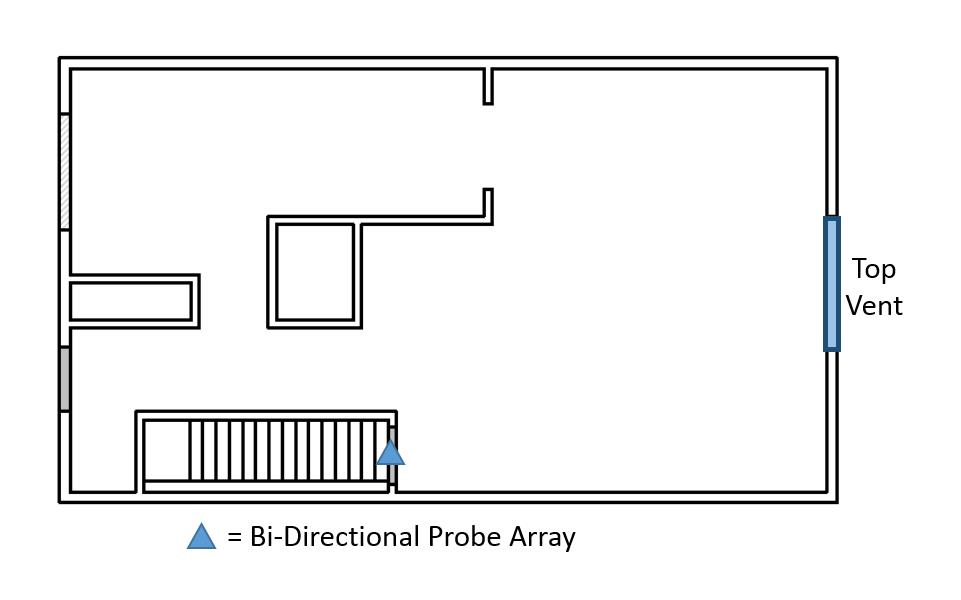
\includegraphics[width=4in]{Figures/Air_Entrainment/Measurement_Location_VentConfig_Top.jpg}
	\caption{Second Floor Ventilation Configuration}
	\label{fig:Second_Floor_Ventilation_Config}
\end{figure}

In order to evaluate how ventilation openings affect the air entrainment due to hose streams, different ventilation openings were considered to include both doors as well as windows of common sizes. The measurement location within the structure was a fixed location and fixed opening size. The measurement location was the size of a common single doorway as seen below. The remainder of the ventilation openings varied between a single and double door as well as a single and double window. Additionally, a controlled door was evaluated to show the impact of a reduced inlet size on the total air entrainment in hose streams. This is a common practice among fire departments based on previous research conducted showing the benefits to closing down the flow path and limiting the available oxygen to the fire. The effect of the controlled door on air entrainment has yet been analyzed and thus was vital to be included in this study.

\vspace*{\baselineskip}

\begin{table}[!ht]
\centering
\begin{tabular}{lccccc|}
\cline{2-6}
\multicolumn{1}{l|}{} & \multicolumn{1}{l|}{\textbf{Width}} & \multicolumn{1}{l|}{\textbf{Height}} & \multicolumn{1}{l|}{\textbf{Width (in)}} & \multicolumn{1}{l|}{\textbf{Height (in)}} & \multicolumn{1}{l|}{\textbf{Area (sq. in.)}} \\ \hline
\multicolumn{1}{|l|}{Measurement Location} & 2' 8" & 6' 8" & 32 & \multicolumn{1}{c|}{80} & 2560 \\ \hline
\multicolumn{1}{|l}{} &  &  &  &  &  \\ \hline
\multicolumn{1}{|l|}{Single Window} & 2' & 4' & 24 & \multicolumn{1}{c|}{48} & 1152 \\
\multicolumn{1}{|l|}{Double Window} & 4' & 5' & 48 & \multicolumn{1}{c|}{60} & 2880 \\
\multicolumn{1}{|l|}{Single Door} & 3' & 6' 8" & 36 & \multicolumn{1}{c|}{80} & 2880 \\
\multicolumn{1}{|l|}{Double Door} & 6' & 6' 8" & 72 & \multicolumn{1}{c|}{80} & 5760 \\
\multicolumn{1}{|l|}{Controlled Door} & 8" & 6' 8" & 8 & \multicolumn{1}{c|}{80} & 640 \\ \hline
\end{tabular}
\caption{Ventilation Opening Sizes}
\label{Vent_Sizes}
\end{table}

% \begin{figure}[!ht]
% 	\centering
% 	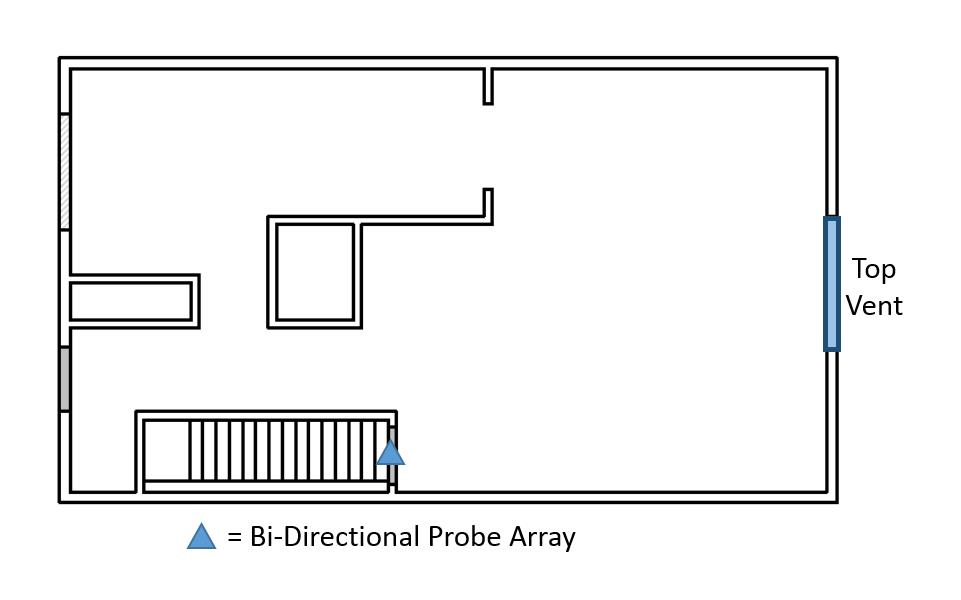
\includegraphics[width=3.5in]{Figures/Air_Entrainment/Measurement_Location_VentConfig_Top.jpg}
% 	\caption{Second Floor Ventilation Configuration}
% 	\label{fig:Second_Floor_Ventilation_Configuration}
% \end{figure}

% \clearpage

\begin{table}[!ht]
\centering
\scalebox{0.8}{
\begin{tabular}{|lccccccc|}
\hline
\multicolumn{1}{|c|}{\textbf{Location}} & \multicolumn{1}{c|}{\textbf{Top Vent}} & \multicolumn{1}{c|}{\textbf{Bottom Vent}} & \multicolumn{1}{c|}{\textbf{Nozzle Size}} & \multicolumn{1}{c|}{\textbf{Nozzle Type}} & \multicolumn{1}{c|}{\textbf{Tip Size}} & \multicolumn{1}{c|}{\textbf{Flow Rate}} & \textbf{Pressure} \\ \hline
Interior & Controlled Door & Single Window & 1.5 & Combination &  & 150 & 75 \\
Interior & Double Door & Double Door & 1.5 & Combination &  & 150 & 75 \\
Interior & Double Door & Single Door & 1.5 & Combination &  & 150 & 75 \\
Interior & Double Door & Single Window & 1.5 & Combination &  & 150 & 75 \\
Interior & No Opening & Double Door & 1.5 & Combination &  & 150 & 75 \\
Interior & No Opening & Single Door & 1.5 & Combination &  & 150 & 75 \\
Interior & No Opening & Single Window & 1.5 & Combination &  & 150 & 75 \\
Interior & Single Door & Double Door & 1.5 & Combination &  & 150 & 75 \\
Interior & Single Door & Single Door & 1.5 & Combination &  & 150 & 75 \\
Interior & Single Door & Double Window & 1.5 & Combination &  & 150 & 75 \\
Interior & Single Door & Single Window & 1.5 & Combination &  & 150 & 75 \\
Interior & Controlled Door & Single Window & 1.5 & Smooth Bore & 15/16 & 180 & 50 \\
Interior & Double Door & Single Window & 1.5 & Smooth Bore & 15/16 & 180 & 50 \\
Interior & Single Door & Double Window & 1.5 & Smooth Bore & 15/16 & 180 & 50 \\
Interior & Single Door & Single Window & 1.5 & Smooth Bore & 15/16 & 180 & 50 \\
Exterior & Double Door & Double Door & 1.5 & Combination &  & 150 & 75 \\
Exterior & Double Door & Single Door & 1.5 & Combination &  & 150 & 75 \\
Exterior & No Opening & Double Door & 1.5 & Combination &  & 150 & 75 \\
Exterior & No Opening & Single Door & 1.5 & Combination &  & 150 & 75 \\
Exterior & No Opening & Single Window & 1.5 & Combination &  & 150 & 75 \\
Exterior & Single Door & Double Door & 1.5 & Combination &  & 150 & 75 \\
Exterior & Single Door & Single Door & 1.5 & Combination &  & 150 & 75 \\
Exterior & Single Door & Double Window & 1.5 & Combination &  & 150 & 75 \\
Exterior & Single Door & Single Window & 1.5 & Combination &  & 150 & 75 \\
Exterior & Single Window & Double Window & 1.5 & Combination &  & 150 & 75 \\
Exterior & Single Window & Single Door & 1.5 & Combination &  & 150 & 75 \\
Exterior & No Opening & Single Window & 1.5 & Smooth Bore & 15/16 & 180 & 50 \\
Exterior & Single Door & Double Window & 1.5 & Smooth Bore & 15/16 & 180 & 50 \\
Exterior & Single Door & Single Window & 1.5 & Smooth Bore & 15/16 & 180 & 50 \\
Exterior & Single Window & Single Door & 2.5 & Combination &  & 250 & 75 \\
Exterior & Single Door & Single Window & 2.5 & Combination &  & 250 & 75 \\
Exterior & Single Window & Single Door & 2.5 & Smooth Bore & 1 1/4 & 320 & 50 \\
Exterior & Single Door & Single Window & 2.5 & Smooth Bore & 1 1/4 & 320 & 50 \\
Exterior & Single Window & Single Door & PM & Combination &  & 500 & 80 \\
Exterior & Single Door & Single Window & PM & Combination &  & 500 & 80 \\
Exterior & Single Window & Single Door & PM & Smooth Bore & 1 3/8 & 500 & 80 \\
Exterior & Single Door & Single Window & PM & Smooth Bore & 1 3/8 & 500 & 80 \\
Transitional & Single Window & Single Window & 1.5 & Combination &  & 150 & 75 \\
Transitional & No Opening & Single Window & 1.5 & Combination &  & 150 & 75 \\
Transitional & Single Door & Single Window & 1.5 & Combination &  & 150 & 75 \\
Transitional & Single Window & Single Window & 1.5 & Smooth Bore & 15/16 & 180 & 50 \\
Transitional & No Opening & Single Window & 1.5 & Smooth Bore & 15/16 & 180 & 50 \\
Transitional & Single Door & Single Window & 1.5 & Smooth Bore & 15/16 & 180 & 50 \\ \hline
\end{tabular}}
\caption{Ventilation Configuration Experiments}
\label{Ventilation_Configuration_Experiments}
\end{table}

\clearpage

\subsubsection{Room Configuration}

The last test series of the air entrainment experiments involved reconfiguring the first floor of the structure to analyze how compartmentation and varying building geometries affect the end result. The air entrainment from various attacks, both fixed position and advancements, was studied. Additionally, the tests were conducted from both the interior and exterior of the structure. The nozzles utilized during these experiments included both a 1.5~in. combination nozzle and a 1.5~in. smooth bore nozzle with a 15/16~in. tip.

The dimensioned drawing below shows the changes to the first floor of the structure. A wall was constructed to create a room adjacent to the bottom ventilation opening. Attached to the room via a standard 2~ft. 6~in. by 6~ft. 8~in. doorway was a 16~ft. by 4~ft. hallway. This allowed for the team to study entrainment in a structure configuration most comparable to residential single family homes. This setup would best simluate the configuration for a suppression crew advancing down a hallway towards a bedroom including single door entry with a window present in the room. 

\begin{figure}[!ht]
	\centering
	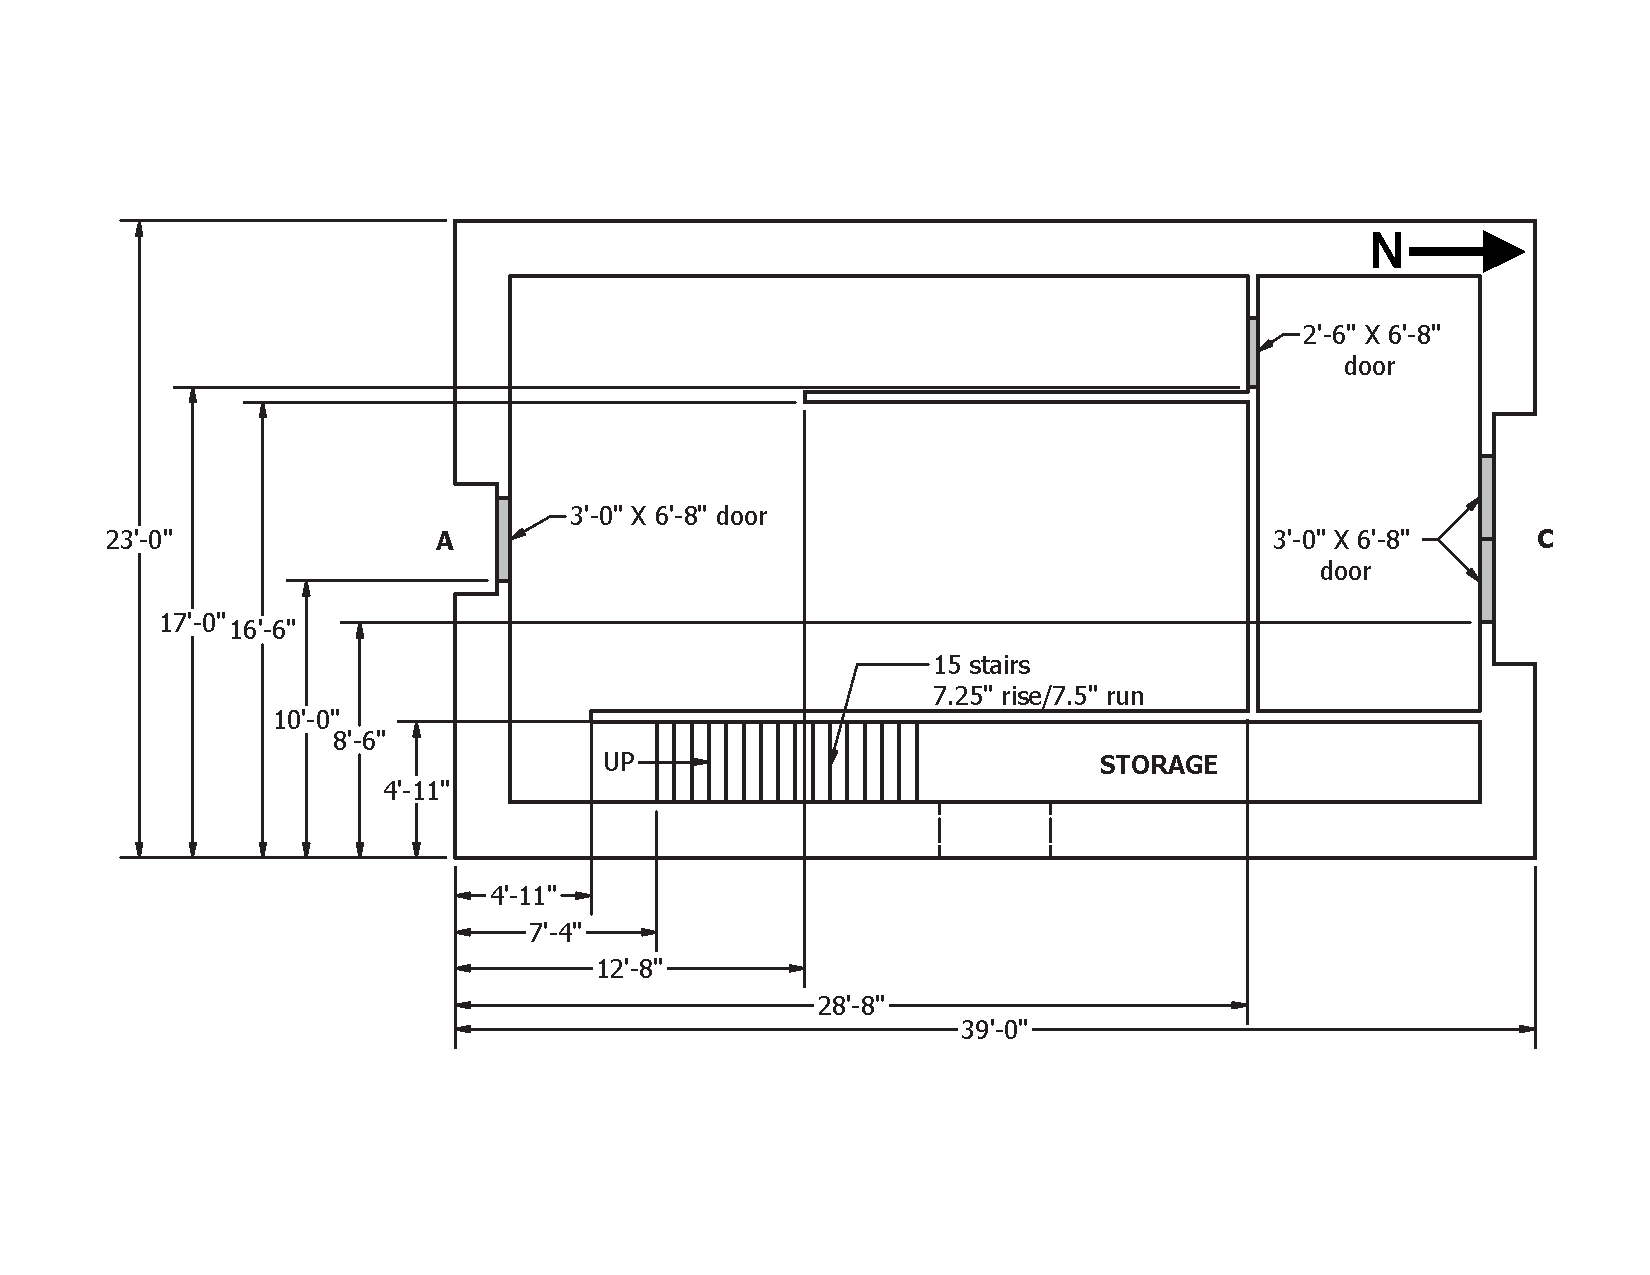
\includegraphics[width=6in]{Figures/Air_Entrainment/West_Test_Structure_1st_Floor_nodim.pdf}
	\caption{First Floor Alterations Room Configuration}
	\label{fig:First_Floor_Alterations_Room_Configuration}
\end{figure}

\clearpage

\begin{figure}[!ht]
	\centering
	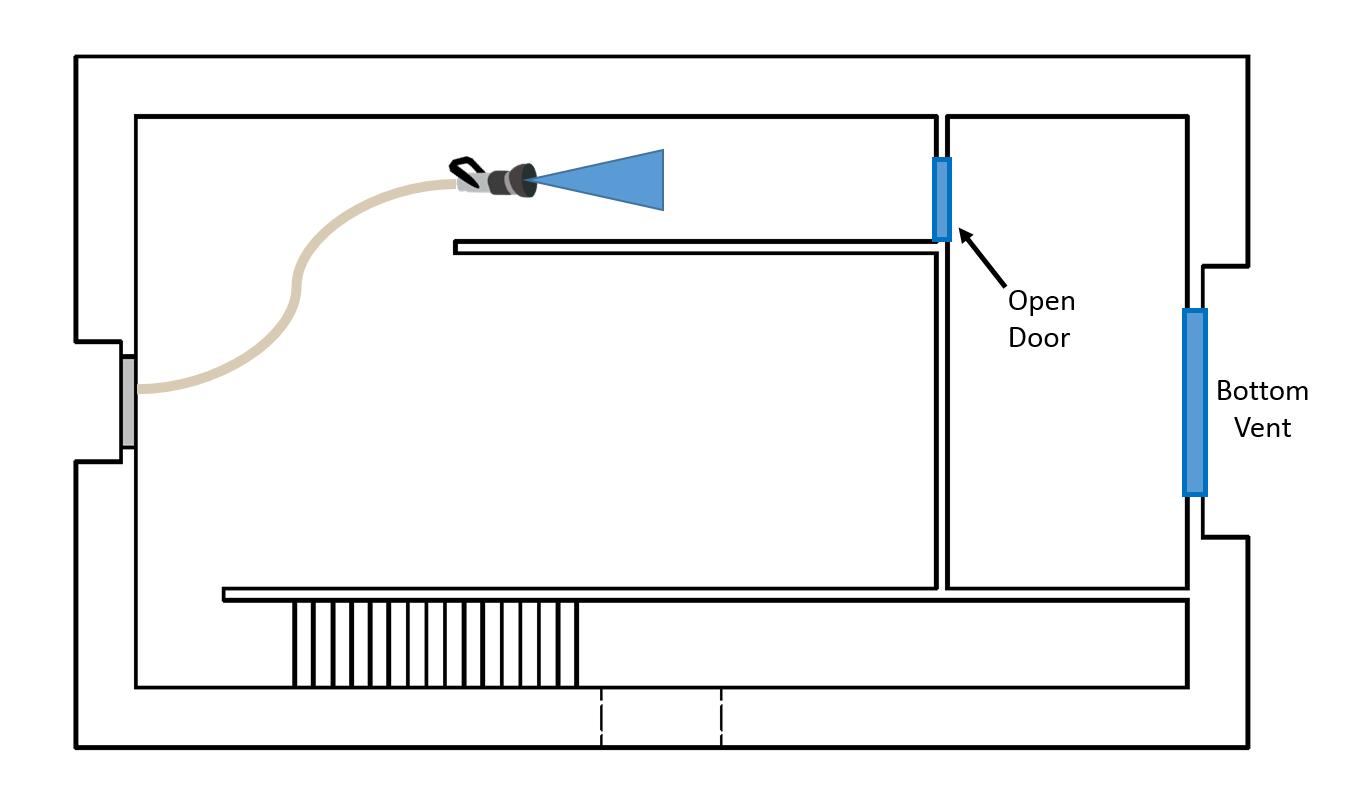
\includegraphics[width=4in]{Figures/Air_Entrainment/Measurement_Location_Room_Configuration_Bottom.jpg}
	\caption{First Floor Room Configuration, Interior Experiments}
	\label{fig:First_Floor_Room_Configuration_Interior_Experiments}
\end{figure}

\begin{figure}[!ht]
	\centering
	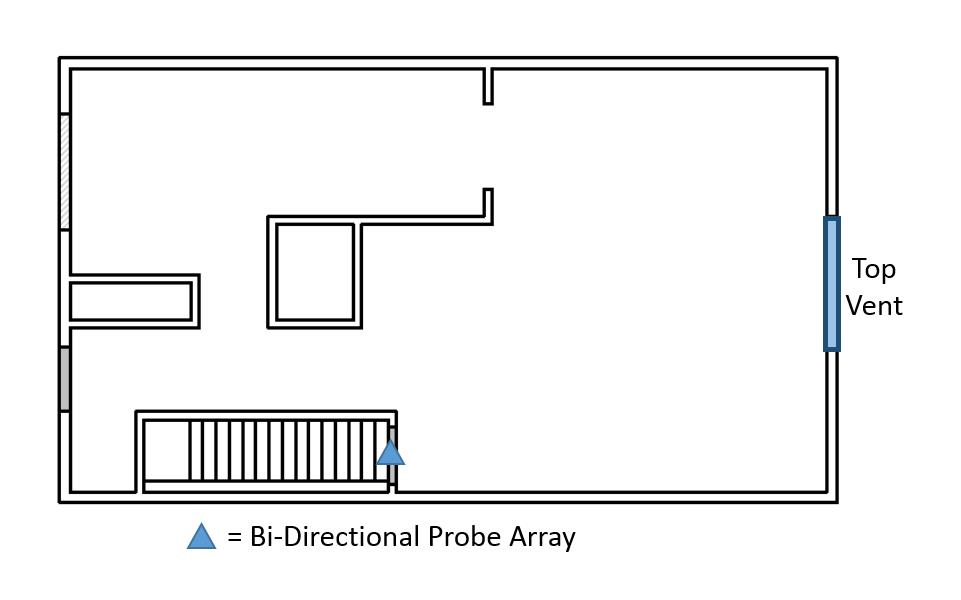
\includegraphics[width=4in]{Figures/Air_Entrainment/Measurement_Location_VentConfig_Top.jpg}
	\caption{Second Floor Room Configuration}
	\label{fig:Second_Floor_Room_Configuration}
\end{figure}

\begin{table}[!ht]
\centering
\begin{tabular}{|lccccc|}
\hline
\multicolumn{1}{|c|}{\textbf{Location}} & \multicolumn{1}{c|}{\textbf{Nozzle Size}} & \multicolumn{1}{c|}{\textbf{Nozzle Type}} & \multicolumn{1}{c|}{\textbf{Tip Size}} & \multicolumn{1}{c|}{\textbf{Flow Rate}} & \textbf{Pressure} \\ \hline
Interior & 1.5 & Smooth Bore & 15/16 & 180 & 50 \\
Interior & 1.5 & Smooth Bore & 15/16 & 180 & 50 \\
Interior & 1.5 & Smooth Bore & 15/16 & 180 & 50 \\
Interior & 1.5 & Combination &  & 150 & 50 \\
Interior & 1.5 & Combination &  & 150 & 50 \\
Interior & 1.5 & Combination &  & 150 & 50 \\
Interior & 1.5 & Combination &  & 150 & 75 \\
Exterior & 1.5 & Combination &  & 150 & 50 \\ \hline
\end{tabular}
\caption{Room Configuration Experiments}
\label{Room_Configuration_Experiments}
\end{table}

\clearpage

\subsection{Analysis \& Results}

\vspace*{\baselineskip}

After the air entrainment testing was complete and the results were analyzed, several conclusions were drawn:

\begin{itemize}
	\item Air entrainment is dependent on hose stream type. (smooth bore, straight stream, fog)
	\item Air entrainment is dependent on structure size, compartmentation, and ventilation configurations.
	\item Increases in nozzle movement increase overall air entrainment.
	\item Different nozzle movement patterns have little effect on overall air entrainment. (O, T, Z, inverted U)
	\item Air entrainment, either into or out of the structure, is dependent on the horizontal distance of the nozzle to the ventilation opening.
\end{itemize}

Each of these conclusions is explained in detail below with supporting results.

\paragraph{Manufacturer Comparison}

\vspace*{\baselineskip}

The table below shows the series of tests that were conducted to compare similar nozzles from differing manufacturers. Within each of these tests, the air entraiment from various hose stream types was determined.

\vspace*{\baselineskip}

\begin{table}[!ht]
\centering
\begin{tabular}{|lcclccc|}
\hline
\multicolumn{1}{|c|}{\textbf{Location}} & \multicolumn{1}{c|}{\textbf{Nozzle Size}} & \multicolumn{1}{c|}{\textbf{Manufacturer}} & \multicolumn{1}{c|}{\textbf{Nozzle Type}} & \multicolumn{1}{c|}{\textbf{Tip Size}} & \multicolumn{1}{c|}{\textbf{Flow Rate}} & \textbf{Pressure} \\ \hline
Interior & 1.5 & MF3 & Combination &  & 95 & 100 \\
Interior & 1.5 & MF3 & Combination &  & 150 & 50 \\
Interior & 1.5 & MF3 & Combination &  & 150 & 75 \\
Interior & 1.5 & MF3 & Combination &  & 150 & 100 \\
Interior & 1.5 & MF3 & Smooth Bore & 7/8 & 150 & 50 \\
Interior & 1.5 & MF3 & Smooth Bore & 15/16 & 180 & 50 \\
Interior & 1.5 & MF3 & Smooth Bore & 1 & 210 & 50 \\
Interior & 1.5 & MF2 & Combination &  & 95 & 100 \\
Interior & 1.5 & MF2 & Combination &  & 150 & 50 \\
Interior & 1.5 & MF2 & Combination &  & 150 & 75 \\
Interior & 1.5 & MF2 & Combination &  & 150 & 100 \\
Interior & 1.5 & MF2 & Smooth Bore & 7/8 & 150 & 50 \\
Interior & 1.5 & MF2 & Smooth Bore & 15/16 & 180 & 50 \\
Interior & 1.5 & MF2 & Smooth Bore & 1 & 210 & 50 \\
Interior & 1.5 & MF1 & Combination &  & 95 & 100 \\
Interior & 1.5 & MF1 & Combination &  & 150 & 50 \\
Interior & 1.5 & MF1 & Combination &  & 150 & 75 \\
Interior & 1.5 & MF1 & Combination &  & 150 & 100 \\
Interior & 1.5 & MF1 & Smooth Bore & 7/8 & 150 & 50 \\
Interior & 1.5 & MF1 & Smooth Bore & 15/16 & 180 & 50 \\
Interior & 1.5 & MF1 & Smooth Bore & 1 & 210 & 50 \\ \hline
\end{tabular}
\caption{Manufacturer Comparison Experiments}
\label{Manufacturer_Comparison_Experiments}
\end{table}

\clearpage

\begin{figure}[!ht]
\begin{tabular*}{\textwidth}{lr}
\includegraphics[width=3.5in]{Script_Figures/Entrainment/Manufacturer_1_5_Combination_Nozzle_95gpm_100psi} &
\includegraphics[width=3.5in]{Script_Figures/Entrainment/Manufacturer_1_5_Combination_Nozzle_150gpm_50psi} \\
\includegraphics[width=3.5in]{Script_Figures/Entrainment/Manufacturer_1_5_Combination_Nozzle_150gpm_75psi} &
\includegraphics[width=3.5in]{Script_Figures/Entrainment/Manufacturer_1_5_Combination_Nozzle_150gpm_100psi} \\
\end{tabular*}
\caption{Figures showing manufacturer comparison of air entrainment results for 1.5 in combination nozzles.}
\label{fig:1_5_Interior_Combination_Manufacturer}
\end{figure}

\clearpage

\begin{figure}[!ht]
\begin{tabular*}{\textwidth}{lr}
\includegraphics[width=3.5in]{Script_Figures/Entrainment/Manufacturer_1_5_Smooth_Bore_Nozzle_7_8_150gpm_50psi} &
\includegraphics[width=3.5in]{Script_Figures/Entrainment/Manufacturer_1_5_Smooth_Bore_Nozzle_15_16_180gpm_50psi} \\
\end{tabular*}
\centering
\includegraphics[width=3.5in]{Script_Figures/Entrainment/Manufacturer_1_5_Smooth_Bore_Nozzle_1_210gpm_50psi} 
\caption{Figures showing manufacturer comparison of air entrainment results for 1.5 in smooth bore nozzles.}
\label{fig:1_5_Interior_Smooth_Bore_Manufacturer}
\end{figure}

As shown by the results for both the 1.5~in. combination and smooth bore nozzles examined, manufacturers have different design details for their given product and that is evident in the differening air entrainment results. The spread amongst manufacturers in the combination nozzle varies anywhere from less than 1000~CFM to over 2000~CFM. Due to the more simple design features of the smooth bore nozzles, the differences across manufacturers was less.

With that being said, several trends were consistent amongst the different experiments:

\begin{itemize}
	\item Increases in nozzle movement (i.e. fixed compared to `O' pattern) increase overall air entrainment.
	\item The wider the hose stream pattern, the larger the amount of air entrained. (i.e. narrow fog when compared to straight stream or smooth bore)
\end{itemize}

\clearpage

\paragraph{Air entrainment is dependent on hose stream type. (smooth bore, straight stream, fog)} \mbox{}

The intial opening occlusion test was conducted to determine how varying the hose stream type from a single nozzle can effect the air entrainment at a given setback distance (3~ft.). This test showed that given a fixed setback distance, a combination nozzle flowing a common flow rate of 150~gpm at a pressure of 50~psi had increasing air entrainment with an increase in the width of the pattern. As the pattern became wider, approaching the size of the ventilation opening, the air entrainment increased, with straight stream experiencing the smallest airflow. 

\begin{figure}[!ht]
	\centering
	\includegraphics[width=4in]{Script_Figures/Entrainment/Opening_Occlusion}
	\caption{Varying air entrainment in varying hose stream types utilizing a 1.5" combination nozzle with a flow rate of 150gpm at 50 psi.}
	\label{fig:Opening_Occlusion}
\end{figure}

Varying the hose stream type was analyzed in various other experiments as well. These were conducted with a interior fixed setback distance of 18~ft. and utilized 1.5" nozzles.

% \vspace*{\baselineskip}

\begin{table}[!ht]
\centering
\begin{tabular}{|lccc|}
\hline
\multicolumn{1}{|c|}{\textbf{Hose Stream Type}} & \multicolumn{1}{c|}{\textbf{Flow Rate (GPM)}} & \multicolumn{1}{c|}{\textbf{Pressure (PSI)}} & \textbf{Air Entrainment (CFM)} \\ \hline
Straight Stream & 150 & 50 & 3440 \\
Straight Stream `O' & 150 & 50 & 10441 \\
Narrow Fog & 150 & 50 & 17645 \\
Narrow Fog `O' & 150 & 50 & 22873 \\
Smooth Bore & 150 & 50 & 3319 \\
Smooth Bore `O' & 150 & 50 & 9738 \\ \hline
\end{tabular}
\caption{Hose stream type comparison for interior 1.5" nozzles.}
\label{Hose_Stream_Type_Comparison}
\end{table}

\clearpage

\paragraph{Air entrainment is dependent on structure size, compartmentation, and ventilation configurations.} \mbox{}

The first set of experiments in which the ventilation openings were examined utilized a 1.5~in. combination (150~gpm @ 75~psi) nozzle and a smooth bore nozzle (15/16" tip, 180~gpm @ 50~psi). Four different intake openings were examined including no door, controlled door, single door, and double door. These were looking at scenarios in which a fire attack crew makes entry into the structure via a doorway and is flowing water towards an exhaust of varying size and shape. A window was not examined as one of the intake openings as the assumption was made that the attack crew would be entering the building through a door and not a window. The distance from the nozzle to the opening was 18~ft.

\begin{figure}[!ht]
\begin{tabular*}{\textwidth}{lr}
\includegraphics[width=3.5in]{Script_Figures/Entrainment/Vent_Configuration_1_5_Combination_Nozzle_Interior_No_Door_Top} &
\includegraphics[width=3.5in]{Script_Figures/Entrainment/Vent_Configuration_1_5_Combination_Nozzle_Interior_Controlled_Door} \\
\includegraphics[width=3.5in]{Script_Figures/Entrainment/Vent_Configuration_1_5_Combination_Nozzle_Interior_Single_Door_Top} &
\includegraphics[width=3.5in]{Script_Figures/Entrainment/Vent_Configuration_1_5_Combination_Nozzle_Interior_Double_Door_Top} \\
\end{tabular*}
\caption{Figures showing interior air entrainment results for 1.5" combination nozzles with fixed intake openings and varying exhaust openings.}
\label{fig:1_5_Interior_Combination_Vents}
\end{figure}

\clearpage

\begin{figure}[!ht]
\centering
\includegraphics[width=4in]{Script_Figures/Entrainment/Vent_Configuration_1_5_Smooth_Bore_Nozzle_Interior}
\caption{Figures showing interior air entrainment results for 1.5" smooth bore nozzles with fixed intake openings and varying exhaust openings.}
\label{fig:1_5_Interior_Smooth_Bore_Vents}
\end{figure}

Several conclusions can be drawn from the first set of ventilation experiments looking at interior attacks:

\begin{itemize}
	\item As the size of the intake opening increases, so does the amount of air entrained into the hose stream.
	\item Controlling the door after entry by the fire attack team significantly reduces the amount of air entrainment.
	\item \hl{Something about exhaust vent sizes}
\end{itemize}

\clearpage

The next set of experiments utilized the same nozzles as the interior attack tests above; however these examined the differences in air entrainment from exterior streams. These tests incorporated fixed exhaust openings and varyied intake shapes and sizes. The distance from the nozzle to the opening was 18~ft.

\begin{figure}[!ht]
\begin{tabular*}{\textwidth}{lr}
\includegraphics[width=3.5in]{Script_Figures/Entrainment/Vent_Configuration_1_5_Combination_Nozzle_Exterior_No_Door_Top} &
\includegraphics[width=3.5in]{Script_Figures/Entrainment/Vent_Configuration_1_5_Combination_Nozzle_Exterior_Single_Window_Top} \\
\includegraphics[width=3.5in]{Script_Figures/Entrainment/Vent_Configuration_1_5_Combination_Nozzle_Exterior_Single_Door_Top} &
\includegraphics[width=3.5in]{Script_Figures/Entrainment/Vent_Configuration_1_5_Combination_Nozzle_Exterior_Double_Door} \\
\end{tabular*}
\caption{Figures showing exterior air entrainment results for 1.5" combination nozzles with fixed exhaust openings and varying intake openings.}
\label{fig:1_5_Exterior_Combination_Vents}
\end{figure}

\clearpage

\begin{figure}[!ht]
\centering
\includegraphics[width=4in]{Script_Figures/Entrainment/Vent_Configuration_1_5_Smooth_Bore_Nozzle_Exterior}
\caption{Figures showing exterior air entrainment results for 1.5" smooth bore nozzles with fixed exhaust openings and varying intake openings.}
\label{fig:1_5_Exterior_Smooth_Bore_Vents}
\end{figure}

Several conclusions can be drawn from the second set of ventilation experiments looking at exterior attacks:

\begin{itemize}
	\item The amount of air entrained into the hose stream and moved throughout the structure is dependent on the size of the available exhaust opening.
	\item The larger the intake opening, the more air available to be entrained into the hose stream.
\end{itemize}

\clearpage

The following experiments looked at the scenario in which a crew would be much closer to the ventilation opening, utilizing exterior streams in what is known as a transitional attack. The fire attack crew would be located on the exterior of the structure, flowing water into the building via a single window. The distance from the nozzle to the opening was less than 3~ft.

\begin{figure}[!ht]
\begin{tabular*}{\textwidth}{lr}
\includegraphics[width=3.5in]{Script_Figures/Entrainment/Vent_Configuration_1_5_Combination_Nozzle_Transitional} &
\includegraphics[width=3.5in]{Script_Figures/Entrainment/Vent_Configuration_1_5_Smooth_Bore_Nozzle_Transitional} \\
\end{tabular*}
\caption{Figures showing transitional air entrainment results for 1.5" nozzles with fixed intake openings and varying exhaust openings.}
\label{fig:1_5_Transitional_Vents}
\end{figure}

Several conclusions can be drawn from this set of ventilation experiments looking at transitional attacks:

\begin{itemize}
	\item The amount of air entrained into the hose stream and moved throughout the structure is dependent on the size of the available exhaust opening.
	\item The larger the exhuast opening, the more air available to be entrained into the hose stream.
\end{itemize}

\clearpage

Several tests were conducted with hose lines of 2.5~in. diameter in which 2.5~in. nozzles were examined as well as portable monitors.

\begin{figure}[!ht]
\begin{tabular*}{\textwidth}{lr}
\includegraphics[width=3.5in]{Script_Figures/Entrainment/Vent_Configuration_2_5_Combination_Nozzle_Exterior} &
\includegraphics[width=3.5in]{Script_Figures/Entrainment/Vent_Configuration_2_5_Smooth_Bore_Nozzle_Exterior} \\
\end{tabular*}
\caption{Figures showing air entrainment results for 2.5" nozzles with varying exhaust and intake openings.}
\label{fig:2_5_Exterior_Vents}
\end{figure}

\begin{figure}[!ht]
\begin{tabular*}{\textwidth}{lr}
\includegraphics[width=3.5in]{Script_Figures/Entrainment/Vent_Configuration_PM_Combination_Nozzle_Exterior} &
\includegraphics[width=3.5in]{Script_Figures/Entrainment/Vent_Configuration_PM_Smooth_Bore_Nozzle_Exterior} \\
\end{tabular*}
\caption{Figures showing air entrainment results for portable monitor nozzles with varying exhaust and intake openings.}
\label{fig:PM_Exterior_Vents}
\end{figure}

\clearpage

% \begin{figure}[!ht]
% 	\centering
% 	\includegraphics[width=4in]{Script_Figures/Entrainment/Vent_Configuration_1_5_Combination_Nozzle_Interior_Controlled_Door}
% 	\caption{Figure showing entrainment results for varying exhaust vent configuration of an interior 1.5" combination nozzle with a fixed controlled door inlet.}
% 	\label{fig:1_5_Interior_Vent_Configuration_Combination_Comparison_Controlled_Door}
% \end{figure}

% \begin{figure}[!ht]
% 	\centering
% 	\includegraphics[width=4in]{Script_Figures/Entrainment/Vent_Configuration_1_5_Combination_Nozzle_Interior_Double_Door_Top}
% 	\caption{Figure showing entrainment results for varying exhaust vent configuration of an interior 1.5" combination nozzle with a fixed double door inlet.}
% 	\label{fig:1_5_Interior_Vent_Configuration_Combination_Comparison_Double_Door_Top}
% \end{figure}

% \begin{figure}[!ht]
% 	\centering
% 	\includegraphics[width=4in]{Script_Figures/Entrainment/Vent_Configuration_1_5_Combination_Nozzle_Interior_Single_Door_Top}
% 	\caption{Figure showing entrainment results for varying exhaust vent configuration of an interior 1.5" combination nozzle with a fixed single door inlet.}
% 	\label{fig:1_5_Interior_Vent_Configuration_Combination_Comparison_Single_Door_Top}
% \end{figure}

% \begin{figure}[!ht]
% 	\centering
% 	\includegraphics[width=4in]{Script_Figures/Entrainment/Vent_Configuration_1_5_Combination_Nozzle_Interior_No_Door_Top}
% 	\caption{Figure showing entrainment results for varying exhaust vent configuration of an interior 1.5" combination nozzle with no door for an inlet.}
% 	\label{fig:1_5_Interior_Vent_Configuration_Combination_Comparison_No_Door_Top}
% \end{figure}

% \clearpage

\paragraph{Increases in nozzle movement increase overall air entrainment}

A single test was conducted to determine the differences in air entrainment when a given 1.5~in. smooth bore nozzle of fixed flow rate of 210~gpm and pressure of 50~psi was utilized with a `O' pattern at different rotation speeds. Using a metronome, the `O' pattern was applied at 50, 100, and 150 revolutions per minute. This test was conducted at the fixed interior setback distance of 18~ft. from the tip of the nozzle to the ventilation opening.

\begin{figure}[!ht]
	\centering
	\includegraphics[width=4in]{Script_Figures/Entrainment/Nozzle_Movement_Comparison_1}
	\caption{Figure showing various rotation speeds of an `O' pattern for an interior 1.5" smooth bore nozzle with a 1" tip.}
	\label{fig:1_5_Interior_Nozzle_Movement_RotationSpeed_Comparison}
\end{figure}

As shown in the figure above, an increase in the rotation speed while applying a specified pattern yeilded an increase in the air entrainment seen within the stream.

\clearpage

Additionally, in various other experiments, both fixed and moving patterns were examined. The results confirm that an increase in movement, increase entrainment. The figure below shows that a narrow fog `O' pattern yields higher entrainment than a fixed narrow fog patter and a straight stream `O' pattern yields higher entrainment than a fixed straight stream pattern.

\begin{figure}[!ht]
	\centering
	\includegraphics[width=4in]{Script_Figures/Entrainment/Total_Entrainment_1_5_Combination_Nozzle_Interior}
	\caption{Figure showing entrainment results of interior 1.5" combination nozzles.}
	\label{fig:1_5_Interior_Combination_Results_Nozzle_Movements}
\end{figure}

\clearpage

\paragraph{Differing nozzle movement patterns have little effect on overall air entrainment.} \mbox{}

Various tests were conducted to determine how different nozzle movements effect the overall air entrainment. Common nozzle movements seen in the fire service today are the `O', `Z', and `n' patterns. Differences in these were examined utilizing nozzles of various flow rates and pressures for both 1.5~in. combination as well as 1.5~in. smooth bore nozzles from the interior of the structure at a fixed setback distance of 18~ft. The results show that there is less than a +/- 1000 CFM difference between the patterns across the various nozzle types and settings.

\begin{figure}[!ht]
\begin{tabular*}{\textwidth}{lr}
\includegraphics[width=3.5in]{Script_Figures/Entrainment/Total_Entrainment_1_5_Combination_Nozzle_Interior_Patterns} &
\includegraphics[width=3.5in]{Script_Figures/Entrainment/Total_Entrainment_1_5_Smooth_Bore_Nozzle_Interior_Patterns} \\
\end{tabular*}
\caption{Figures showing air entrainment given various nozzle movements for interior 1.5" nozzles.}
\label{fig:1_5_Interior_Nozzle_Movement_Comparison}
\end{figure}

\clearpage

A test was also conducted to determine if a standard utilized nozzle movement in an `O' pattern would differ from a `Spray and Pray' technique in which the nozzle operator moves the hose stream across the ventilation opening as fast as possible with no discerible pattern. Once again, the results showed little to no difference in the air entrainment.

\begin{figure}[!ht]
	\centering
	\includegraphics[width=4in]{Script_Figures/Entrainment/Nozzle_Movement_Comparison_2}
	\caption{Figure showing common pattern compared to no discernible pattern for an interior 1.5" smooth bore nozzle with a 1" tip.}
	\label{fig:1_5_Interior_Nozzle_Movement_PatterntoNoPattern_Comparison}
\end{figure}

Because the results very clearly showed little to no difference in air entrainment from varying nozzle movements across multiple nozzle types and settings, a single nozzle movement pattern (`O') was utilized for the remainder of the experiments conducted.

\clearpage

\paragraph{Air entrainment is dependent on the distance of the nozzle to the ventilation opening.} \mbox{}

One of the preliminary experiments conducted was the setback comparison tests in which a 1.5~in. combination nozzle at two different pressures (100~psi and 50~psi) was utilized in a fixed pattern at varying distances from the ventilation opening. The nozzle was moved back from the opening at intervals 3, 6, 9, 12, and 15~ft. to see the effect on air entrainment in the hose stream.

\begin{figure}[!ht]
	\centering
	\includegraphics[width=4in]{Script_Figures/Entrainment/Setback_Distance_Comparison}
	\caption{1.5" Combination Nozzle, Setback Distance Comparison}
	\label{fig:1_5_Combination_Nozzle_Setback_Distance_Comparison}
\end{figure}

With a fixed nozzle movement, the tests showed that increasing the distance between the tip of the nozzle and the ventilation opening increased the entrainment in the hose stream. The further the nozzle from the vent allowed for a more broken and `wider' stream, which in turn, encompassed more of the opening.

\vspace*{\baselineskip}

\clearpage

\section{Water Distribution Experiments}

The experiments to determine the distribution of water within a compartment consisted of several test series to gain a wholelistic view of how varying different components, either with the structure or equipment utilized, affected the end result.

\subsection{Test Setup}

\subsubsection{Structures}

Testing for the water distribution experiments was conducted at the UL - Headquarters in Northbrook, IL. A purpose built compartment with a small attached hallway and moveable staircase was constructed to sit atop the ADD apparatus.

\begin{figure}[!ht]
	\centering
	\includegraphics[width=4in]{Figures/Water_Distribution/Building.jpg}
	\caption{Water Distribution Test Structure and ADD Apparatus}
	\label{fig:Water_Distribution_Test_Structure_and_ADD_Apparatus}
\end{figure}

The elevated compartment was build on an existing concrete slab located in one of the rooms within the UL large fire lab. It was designed to simulate a room of size commonly found in residential structures. The size and orientation of the ADD apparatus dictated the overall size of the compartment which measured 15~ft 4~in. by 10~ft 5~in. finished interior dimensions. The compartment was wood frame construction with 2~in. by 4~in. studs and track set to 16~in. centers with a interior height measuring 8~ft 1 1/8~in. rough. The walls and ceiling were lined with 1/2~in. durarock cement board atop 1/2~in. plywood. The ceiling joists were 2~in. by 6~in. set to 16~in. on center. 

\clearpage

\begin{figure}[!ht]
	\centering
	\includegraphics[width=4in]{Figures/Water_Distribution/floor3.jpg}
	\caption{ADD Interior Layout with Flashing}
	\label{fig:ADD_Flashing}
\end{figure}

There was no floor constructed in the compartment as the top of the ADD aparatus served as such. The gaps between the collection bins were covered by flashing which was folded to divert the water evenly in each bin to ensure adequate distribution results. The gaps between the outer collection bins and the walls of the structure were also covered with flashing to ensure all water directed into the structure was collected in the appropriate bins. The interior layout of the structure and use of flashing can be seen in Figure \ref{fig:ADD_Flashing}. 

The compartment featured two ventilation openings, one doorway measuring 3~ft by 6~ft 8~in. which opens to the interior hallway, and one window measuring 2~ft by 4~ft which opens to the exterior of the compartment. A moveable staircase and landing was constructed to provide access to either the interior hallway of the compartment or provide a simulation of a first floor exterior attack. The dimensions of the both the staircase and overall compartment can be seen in the dimensioned drawings below.

\begin{figure}[!ht]
	\centering
	\includegraphics[width=5.5in]{Figures/Water_Distribution/ADDtopviewprint}
	\caption{ADD Top View}
	\label{fig:ADD_Top_View}
\end{figure}

\clearpage

\begin{figure}[!ht]
	\centering
	\includegraphics[width=5.5in]{Figures/Water_Distribution/ADDsideviewprint}
	\caption{ADD Side View}
	\label{fig:ADD_Side_View}
\end{figure}

\clearpage

\subsubsection{Instrumentation}

In order to obtain the results for Part I of this study, sensors were installed in the test fixtures to record measurements throughout the experiments. The instrumentation used varied between the air entrainment and the water distribution testing. The instrtuments, and associated uncertainty, used for each test series is outlined below.

UL operates a fire sprinkler spray density measurement instrument known as the Actual Delivered Density (ADD) apparatus. The first prototype of the apparatus was built at Factory Mutual in mid-1980’s, in order to enable manufacturers to design sprinklers that are effective at ever-increasing commodity storage heights \hl{[1, 2]}. The UL ADD apparatus, constructed in 2003, represents the 3rd generation design within the sprinkler industry. 
 
% \begin{figure}[!ht]
% 	\centering
% 	\includegraphics[width=4in]{Figures/Water_Distribution/ADD.jpg}
% 	\caption{The Actual Delivered Density (ADD) Apparatus Simulating a 2.5 MW Fire}
% 	\label{fig:ADD_Apparatus_Simulating_fire}
% \end{figure}

The concept of the ADD measurement is to simulate the top surface of an array of high storage commodity, and measure the flux of water on this top surface as a result of the spray pattern discharged by one or more sprinklers. The ADD apparatus is designed to perform these measurements while simulating different sized rack storage fires (500~kW to 2.5~MW, in increments of 500~kW). This allows for insight into the effect of a real fire plume on sprinkler spray distribution. Typically, the ADD apparatus is used to simulate commodity underneath one, between two, or between four fire sprinklers. For sprinkler manufacturers, the ADD apparatus can be used as a screening tool for new automatic sprinkler designs. The fire capabilities were not utilized during any of the water distribution experiments.

% Figure \ref{fig:ADD_Apparatus_Simulating_fire} is a photograph of the UL ADD apparatus in operation.

The UL ADD apparatus is comprised of one main array and two satellite arrays of heavy steel framework. The main array consists of 32 water barrels and water pan collection assemblies while each satellite array contains 8 barrels and collection assemblies. All barrels are of 30-gallon capacity and are connected by a 2-inch diameter hose to a 20 inch by 20 inch inverted square pyramid shaped stainless steel water collection pan above. In total, there are 48 total collection pans/barrels. Differential pressure transducers connect to the bottom of each water collection barrel via flexible tubing. The water level in a given barrel is determined by the head pressure measured by the transducer. The water collection rate is calculated based the change in head pressure over time. As Figure \ref{fig:Top-down schematic view of the ADD apparatus} shows, collection assemblies are arranged into 2x2 arrays so that each group of 4 collection assemblies represents one pallet load of commodity.

\begin{figure}[!ht]
	\centering
	\includegraphics[width=6in]{Figures/Water_Distribution/addschematic}
	\caption{Top-down schematic view of the ADD apparatus}
	\label{fig:Top-down schematic view of the ADD apparatus}
\end{figure}

\begin{figure} [H]
	\centering
	\begin{tabular}{c c}
		\subfloat[Collection Barrels]{\includegraphics[height = 2in]{Figures/Water_Distribution/ADD2.jpg}} &
		\subfloat[Collection Pans]{\includegraphics[height = 2in]{Figures/Water_Distribution/ADDbottom3.jpg}} \\
	\end{tabular}
	\caption{ADD Collection Assembly}
	\label{fig:ADD_Collection_Assembly}
\end{figure}

\clearpage
 
Each collection barrel is also connected to a pneumatic drain valve which can be actuated to automatically drain each barrel at the conclusion of each experiment. Figure \ref{fig:Top-down schematic view of the ADD apparatus} also shows flue spaces, as well as an 8 inch duct in the center of the array, which enable the entrainment necessary to simulate a rack-storage fire. A blower supplies air to the center duct to simulate the momentum of the plume of a fire that has reached the top of a rack storage array. Within the center flue spaces of the main array, 12 spray nozzles are angled toward the center to provide the heptane spray used to simulate the commodity fire. Each of the three arrays contains a pipe network and water spray nozzles for cooling the underside of the water collection pans. Cooling is providing during fire simulation to prevent measurement error due to the evaporation of collected water from the hot steel pans, and to prevent absorbed thermal energy from damaging the steel pans.

Data was collected in order to estimate the uncertainty associated with the water distribution experiments performed using the ADD apparatus. Each water collection assembly was filled to capacity while recording pressure transducer measurements as well as data from a calibrated turbine flowmeter (with less than 1~\% measurement uncertainty).
Although the design of each water collection assembly is the same, the measurement performance across the entire apparatus varied in terms of bias and precision. Overall, the water collection assemblies reported volume with a bias of 0.5 gallons less than the volume calculated using the flow meter and with a precision of +/- 2.4 gallons. Using the same data, it is estimated that the real-time (1 Hz) flowrate calculated by the ADD apparatus reported 0.1 gpm less than the turbine flow meter, and with a precision +/- 0.4 gpm.

The recorded data was used to compute a total amount of water in a given bin with the units of gallons.

\clearpage

\subsubsection{Measurement Locations}

In order to collect the data needed for this analysis, sensors were installed and measurements were recorded throughout each structure. The measurement locations varied dependent on the structure and desired information.

The Actual Delivered Density apparatus, described above, was utilized to measure the amount and dsitribution of water flowed into the compartment constructed specifically for this testing. By placing the ADD apparatus beneath the compartment, all of the water flowed was collected and measured. The collection bins were numbered according to their location within the apparatus which allowed a 3D map of the water flow to show the distribution.

\begin{figure}[!ht]
	\centering
	\includegraphics[width=6in]{Figures/Water_Distribution/Measurement_Locations_BinNumbers}
	\caption{Bin Numbers and Locations}
	\label{fig:Bin Numbers and Locations}
\end{figure}

\clearpage

\subsubsection{Equipment Used}

In order to ensure the data collected and associated results were applicable to the majority of the fire servce, our technical panel was tasked with creating a list of represetative nozzles, specified flows/pressures, and hose line techniques. All of these variables were tested during both the air entrainment and water distribution experiments; however, several other aspects were held constant such as the length of hose used. The nozzles utilized during these experiments can be seen in the table below.

\begin{table}[]
\centering
\begin{tabular}{|llccc|}
\hline
\multicolumn{1}{|l|}{\textbf{Line Size}} & \multicolumn{1}{l|}{\textbf{Nozzle}} & \multicolumn{1}{l|}{\textbf{Tip (in)}} & \multicolumn{1}{l|}{\textbf{Nozzle Pressure (psi)}} & \textbf{Approximate Flow Rate (gpm)} \\ \hline
1 3/4 in. & Smooth Bore & 1 & 50 & 210 \\
 & Smooth Bore & 15/16 & 50 & 180 \\
 & Smooth Bore & 7/8 & 50 & 150 \\
 & Fog &  & 100 & 100 \\
 & Fog &  & 100 & 150 \\
 & Fog &  & 75 & 150 \\
 & Fog &  & 50 & 150 \\ \hline
2 1/2 in. & Smooth Bore & 1 1/8 & 50 & 260 \\
 & Smooth Bore & 1 1/4 & 50 & 320 \\
 & Fog &  & 100 & 250 \\
 & Fog &  & 75 & 250 \\
 & Fog &  & 50 & 250 \\ \hline
Portable Monitor & Smooth Bore & 1 3/8 & 80 & 500 \\
 & Fog &  & 75 & 500 \\ \hline
Master Stream & Smooth Bore & 1 1/2 & 80 & 600 \\
 & Smooth Bore & 1 3/4 & 80 & 800 \\
 & Fog &  & 100 & 500-1000 \\ \hline
\end{tabular}
\caption{Nozzle Selection}
\label{Nozzle Selection}
\end{table}

\clearpage

\subsection{Experiments Conducted}

The water distribution experiments incorporated both interior and exterior fire attack utilizing the various nozzles and configurations chosen by the technical panel. 

The interior testing was simulating a fire on the same floor as the attack crew in which the suppression operations were conducted from an adjoining room/hallway. At this position, the nozzle type as well as nozzle direction and application pattern were varied to determine the water distribution within the compartment. The nozzle directions and associated terminology can be seen in Figure \ref{fig:Nozzle_Direction_Interior_Attack}.

\begin{figure}[!ht]
	\centering
	\includegraphics[width=6in]{Figures/Water_Distribution/Nozzle_Position_Int}
	\caption{Nozzle Direction, Interior Attack}
	\label{fig:Nozzle_Direction_Interior_Attack}
\end{figure}

\clearpage

\begin{table}[]
\centering
\scalebox{0.7}{
\begin{tabular}{|lccccc|}
\hline
\multicolumn{1}{|c|}{\textbf{Nozzle Position}} & \multicolumn{1}{c|}{\textbf{Nozzle Pattern}} & \multicolumn{1}{c|}{\textbf{Nozzle Direction}} & \multicolumn{1}{c|}{\textbf{Nozzle Type}} & \multicolumn{1}{c|}{\textbf{Nozzle Pressure (psi)}} & \textbf{Flow Rate (gpm)} \\ \hline
At Room Entrance & Fixed & Mid Ceiling & Straight Stream & 100 & 125 \\
At Room Entrance & O & Mid Ceiling & Straight Stream & 100 & 125 \\
At Room Entrance & Z & Mid Ceiling & Straight Stream & 100 & 125 \\
At Room Entrance & T & Mid Ceiling & Straight Stream & 100 & 125 \\
At Room Entrance & Inverted U & Mid Ceiling & Straight Stream & 100 & 125 \\
At Room Entrance & Fixed & Mid Ceiling & Fog & 100 & 125 \\
At Room Entrance & Fixed & Mid Ceiling & Straight Stream & 100 & 150 \\
At Room Entrance & O & Mid Ceiling & Straight Stream & 100 & 150 \\
At Room Entrance & Fixed & Mid Ceiling & Fog & 100 & 150 \\
At Room Entrance & O & Mid Ceiling & Fog & 100 & 150 \\
At Room Entrance & Fixed & Mid Ceiling & Straight Stream & 75 & 150 \\
At Room Entrance & O & Mid Ceiling & Straight Stream & 75 & 150 \\
At Room Entrance & Fixed & Mid Ceiling & Fog & 75 & 150 \\
At Room Entrance & O & Mid Ceiling & Fog & 75 & 150 \\
At Room Entrance & Fixed & Mid Ceiling & Straight Stream & 50 & 150 \\
At Room Entrance & O & Mid Ceiling & Straight Stream & 50 & 150 \\
At Room Entrance & Fixed & Mid Ceiling & Fog & 50 & 150 \\
At Room Entrance & O & Mid Ceiling & Fog & 50 & 150 \\
At Room Entrance & Fixed & At Wall & 15/16 Smooth Bore & 50 & 180 \\
At Room Entrance & O & At Wall & 15/16 Smooth Bore & 50 & 180 \\
At Room Entrance & Fixed & Mid Ceiling & 15/16 Smooth Bore & 50 & 180 \\
At Room Entrance & O & Mid Ceiling & 15/16 Smooth Bore & 50 & 180 \\
At Room Entrance & Fixed & Max Angle & 15/16 Smooth Bore & 50 & 180 \\
At Room Entrance & O & Max Angle & 15/16 Smooth Bore & 50 & 180 \\
At Room Entrance & Fixed & At Wall & Straight Stream & 100 & 150 \\
At Room Entrance & O & At Wall & Straight Stream & 100 & 150 \\
At Room Entrance & Fixed & Max Angle & Straight Stream & 100 & 150 \\
At Room Entrance & O & Max Angle & Straight Stream & 100 & 150 \\
At Room Entrance & O & Mid Ceiling & Fog & 100 & 125 \\  \hline
\end{tabular}}
\caption{Interior Fire Attack Distribution Experiments}
\label{Interior_Fire_Attack_Distribution_Experiments}
\end{table}

\clearpage

The exterior testing included both an attack from the fire floor as well as the floor below. These were referred to as first floor and second floor attacks for the purpose of this testing. The construction of the compartment featured a moveable staircase to allow for the variation between first floor and second floor suppression. The exterior testing simulated a single room of fire in which a transitional, or exterior attack, was made by suppression crews. As done in the interior testing, both the nozzle type as well as the nozzle direction and application pattern were varied for comparison. The differences in first floor and second floor attacks can been seen in Figures \ref{fig:Nozzle_Direction_Exterior_1st_Floor_Attack} and \ref{fig:Nozzle_Direction_Exterior_2nd_Floor_Attack}.

\begin{figure}[!ht]
	\centering
	\includegraphics[width=6in]{Figures/Water_Distribution/Nozzle_Position_ExtFirstfloor}
	\caption{Nozzle Direction, Exterior 1st Floor Attack}
	\label{fig:Nozzle_Direction_Exterior_1st_Floor_Attack}
\end{figure}

\begin{figure}[!ht]
	\centering
	\includegraphics[width=6in]{Figures/Water_Distribution/Nozzle_Position_ExtSecondfloor}
	\caption{Nozzle Direction, Exterior 2nd Floor Attack}
	\label{fig:Nozzle_Direction_Exterior_2nd_Floor_Attack}
\end{figure}

\clearpage

\begin{table}[]
\centering
\scalebox{0.7}{
\begin{tabular}{|lccccc|}
\hline
\multicolumn{1}{|c|}{\textbf{Nozzle Position}} & \multicolumn{1}{c|}{\textbf{Nozzle Pattern}} & \multicolumn{1}{c|}{\textbf{Nozzle Direction}} & \multicolumn{1}{c|}{\textbf{Nozzle Type}} & \multicolumn{1}{c|}{\textbf{Nozzle Pressure (psi)}} & \textbf{Flow Rate (gpm)} \\ \hline
Second Floor & Fixed & Max Angle & 15/16 Smooth Bore & 50 & 180 \\
Second Floor & Sweeping & Max Angle & 15/16 Smooth Bore & 50 & 180 \\
Second Floor & Fixed & Mid Ceiling & 15/16 Smooth Bore & 50 & 180 \\
Second Floor & Fixed & Min Angle: Ceiling & 15/16 Smooth Bore & 50 & 180 \\
Second Floor & Fixed & Min Angle: Wall & 15/16 Smooth Bore & 50 & 180 \\
Second Floor & Fixed & Max Angle & 7/8 Smooth Bore & 50 & 150 \\
Second Floor & Fixed & Max Angle & 1 Smooth Bore & 50 & 210 \\
Second Floor & Fixed & Max Angle & Straight Stream & 100 & 150 \\
Second Floor & Sweeping & Max Angle & Straight Stream & 100 & 150 \\
Second Floor & Wide Sweep & Max Angle & Straight Stream & 100 & 150 \\
Second Floor & Fixed & Max Angle: Sill & Straight Stream & 100 & 150 \\
Second Floor & Fixed & Mid Ceiling & Straight Stream & 100 & 150 \\
Second Floor & Fixed & Min Angle: Ceiling & Straight Stream & 100 & 150 \\
Second Floor & Fixed & Min Angle: Wall & Straight Stream & 100 & 150 \\
Second Floor & Fixed & Max Angle & Fog & 100 & 150 \\
Second Floor & Comb (Fixed then O) & Max Angle & Fog & 100 & 150 \\
First Floor & Fixed & Max Angle & 15/16 Smooth Bore & 50 & 180 \\
First Floor & Sweeping & Max Angle & 15/16 Smooth Bore & 50 & 180 \\
First Floor & Fixed & Mid Ceiling & 15/16 Smooth Bore & 50 & 180 \\
First Floor & Fixed & Min Angle: Ceiling & 15/16 Smooth Bore & 50 & 180 \\
First Floor & Fixed & Min Angle: Wall & 15/16 Smooth Bore & 50 & 180 \\
First Floor & Fixed & At Wall & 15/16 Smooth Bore & 50 & 180 \\
First Floor & Fixed & Max Angle & 7/8 Smooth Bore & 50 & 150 \\
First Floor & Fixed & Max Angle & 1 Smooth Bore & 50 & 210 \\
First Floor & Fixed & Max Angle & Straight Stream & 100 & 150 \\
First Floor & Sweeping & Max Angle & Straight Stream & 100 & 150 \\
First Floor & Wide Sweep & Max Angle & Straight Stream & 100 & 150 \\
First Floor & Fixed & Mid Ceiling & Straight Stream & 100 & 150 \\
First Floor & Fixed & Min Angle: Ceiling & Straight Stream & 100 & 150 \\
First Floor & Fixed & Min Angle: Wall & Straight Stream & 100 & 150 \\
First Floor & Fixed & At Wall & Straight Stream & 100 & 150 \\
First Floor & Fixed & Max Angle & Fog & 100 & 150 \\
First Floor & Comb (SS then Fog O) & Max Angle & Fog & 100 & 150 \\
First Floor & Fixed & Max Angle & Straight Stream & 100 & 250 \\
First Floor & Fixed & Min Angle: Ceiling & Straight Stream & 100 & 250 \\
First Floor & Fixed & Max Angle & 1 1/4 Smooth Bore & 50 & 260 \\
First Floor & Fixed & Max Angle & Straight Stream & 100 & 150 \\
First Floor & Fixed & Max Angle & Straight Stream & 100 & 150 \\
First Floor & Fixed & Max Angle & Straight Stream & 100 & 150 \\
First Floor & Fixed & Max Angle & Straight Stream & 100 & 150 \\
First Floor & Fixed & Max Angle & Straight Stream & 100 & 150 \\
First Floor & Fixed & Max Angle & 15/16 Smooth Bore & 50 & 180 \\
First Floor & Fixed & Max Angle & 15/16 Smooth Bore & 30 & 150 \\
First Floor & Fixed & Max Angle & 15/16 Smooth Bore & 15 & 130 \\
First Floor & Fixed & Max Angle & 15/16 Smooth Bore & 10 & 100 \\
First Floor & Fixed & Max Angle & Straight Stream & 50 & 150 \\
First Floor & Fixed & Max Angle & Straight Stream & 75 & 60 \\
First Floor & Fixed & Max Angle & Straight Stream & 50 & 185 \\
First Floor & Fixed & Max Angle & Straight Stream & 25 & 130 \\ \hline
\end{tabular}}
\caption{Exterior Fire Attack Distribution Experiments}
\label{Exterior_Fire_Attack_Distribution_Experiments}
\end{table}

\clearpage

\subsection{Analysis \& Results}

The results from the water distribution testing yielded several tactical considerations for suppression operations on the fireground. These are outlined below along with examples from the results. There are several key points to keep in mind when viewing the analysis. 

The experiments conducted for water distribution were approximately 1 minute in length. This was dictated by the size of the collection barrels in the ADD apparatus. Each collection barrel was a total of 30 gallons. At the start of each test, there was a predetermined amount of water in the bottom of the barrel to ensure the sensors were able to record the intial water received during the testing. This `predetermined' amount of water was recorded prior to the start of the test and was subtracted from the final total so that the end results were not affected by the measurement technique. 

Because of these limitations, the results were only plotted to 20 gallons to minimize uncertainty. Additionally, various bins in various tests only received a final total of a couple gallons or less, and thus, appending the charts to 20 gallons, allows the viewer to more easily see these results. Please keep in mind that the intent of the testing was to determine the location of where water is going within the compartment and not necessarily the total quantity of water that reached a given area. As such, focus on the overall distribution and not the amount of water to a given area.
\subsubsection{Repeatability}

It should be noted that several tests were conducted to determine the repeatability of the experiments to ensure accuracy in the results as well as several tests utilizing `live-fire' in order to detemine the applicability of this testing to the remainder of the study.

Four tests utilizing a straight stream nozzle flowing 150~gpm at 100~psi from the exterior first floor position directed into the structure with a maximum angle were conducted to determine the variance in results.

\clearpage 

\begin{figure}[ht]
\begin{tabular*}{\textwidth}{lr}
\includegraphics[width=3.2in]{Script_Figures/ADD_Analysis/15-12-10_082039_Datafile_Straight_Stream_Exterior} &
\includegraphics[width=3.2in]{Script_Figures/ADD_Analysis/15-12-10_082423_Datafile_Straight_Stream_Exterior} \\
\includegraphics[width=3.2in]{Script_Figures/ADD_Analysis/15-12-10_083305_Datafile_Straight_Stream_Exterior} &
\includegraphics[width=3.2in]{Script_Figures/ADD_Analysis/15-12-10_083751_Datafile_Straight_Stream_Exterior} \\
\end{tabular*}
\caption{Figures showing repeatability in test results.}
\label{fig:Repeatability_Testing}
\end{figure}

\vspace*{\baselineskip}

From these results, it is clear that the differences between the tests were minimal and thus determined that the measurement technique was repeatable.

\clearpage

% \subsubsection{Comparison to Fire Testing}

% Additionally, two tests were conducted using `live fire' in which two UL 199 standard commodity wooden cribs were placed in the center of the compartment, as shown in Figure \ref{fig:Wood_Crib_Location}, atop a collection pan filled with heptane. The wooden cribs were chosen because of their ability to maintain a near constant burn rate for a period of time. Wooden cribs have been used in the standards testing of sprinklers for many years. The wood cribs were constructed of kiln-dried spruce or fir sticks measuring 1.5~in. high by 1.5~in. wide by 20~in. long. These were fastened together with nails and stacked atop one another to form the overal structure (10 alternating layers, with 5 sticks per layer). The crib measured 20~in. wide by 20~in. deep by 15~in. high and weighed approximately 33~lbs. each. Two cribs were stacked atop one another to ensure the steady burning period of the fire would last for the duration of the experiment. In order to shorten the time to reach the steady burning period and assist in the near uniform ignition of the cribs, 32~oz of Heptane was poured in the pan beneath and ignited with a propane torch.

% \begin{figure}[!ht]
% 	\centering
% 	\includegraphics[width=4in]{Figures/Water_Distribution/ADDcriblocation.jpg}
% 	\caption{Wood Crib Location}
% 	\label{fig:Wood_Crib_Location}
% \end{figure}

% \begin{figure} [H]
% 	\centering
% 	\begin{tabular}{c c}
% 		\subfloat[Wooden Cribs]{\includegraphics[height = 2.5in]{Figures/Water_Distribution/WoodCrib2.jpg}} &
% 		\subfloat[Fire Test]{\includegraphics[height = 2.5in]{Figures/Water_Distribution/WoodCribfire3.jpg}} \\
% 	\end{tabular}
% 	\caption{ADD Fire Tests}
% 	\label{fig:ADD_Fire_Tests}
% \end{figure}

% \clearpage

% The results of the two fire tests are shown below as compared to the same tests conducted without `live fire.'

% \vspace*{\baselineskip}

% \begin{figure}[ht]
% \begin{tabular*}{\textwidth}{lr}
% \includegraphics[width=3.2in]{Script_Figures/ADD_Analysis/15-12-10_132600_Datafile_Straight_Stream_Interior} &
% \includegraphics[width=3.2in]{Script_Figures/ADD_Analysis/15-12-09_152435_Datafile_Straight_Stream_Interior} \\
% \includegraphics[width=3.2in]{Script_Figures/ADD_Analysis/15-12-10_122043_Datafile_Straight_Stream_Exterior} &
% \includegraphics[width=3.2in]{Script_Figures/ADD_Analysis/15-12-08_113237_Datafile_Straight_Stream_Exterior} \\
% \end{tabular*}
% \caption{`Live fire' comparison results.}
% \label{fig:Live_Fire_Comparison}
% \end{figure}

% From these results, it was determined that the distributions were similar with or without the presence of fire. The small differences can be attributed to several aspects of the testing, including:

% \begin{itemize}
% 	\item As the water passes into the heated compartment and contacts the hot gas layer, some of the water is converted to steam as it heats up and thus the total quantity of water making it into the bins will be slightly smaller in the fire tests.
% 	\item The collection bins immediately adjacent to the bin where the wooden cribs were placed showed a higher amount of water collected in the fire tests when compared to those without fire. This is attributed to some of the water deflecting off of the crib and falling into the bins surrounding the crib.
% \end{itemize}

% If the attack is made from either the interior or exterior of the structure and the stream is directed at the ceiling, the majority of the water `rides' down the opposite wall from the nozzle location, with little to no water making it into the center of the compartment.

% \clearpage

\paragraph{Water distribution is dependent on nozzle type (smooth bore, straight stream, fog).} \mbox{}

% ------------------------------------------------------------------------------------
% Interior
% ------------------------------------------------------------------------------------

% Interior (at room entrance, fixed pattern, set flow/pressure)
% 	SS (150 @ 50), Fog (150 @ 50), 15/16 SB (180 @ 50)
% 	15-12-09_121955_Datafile, 15-12-09_123142_Datafile, 15-12-09_144839_Datafile

\begin{figure}[ht]
\begin{tabular*}{\textwidth}{lr}
\includegraphics[width=3.2in]{Script_Figures/ADD_Analysis/15-12-09_121955_Datafile_Straight_Stream_Interior} &
\includegraphics[width=3.2in]{Script_Figures/ADD_Analysis/15-12-09_123142_Datafile_Fog_Interior} \\
\end{tabular*}
\centering
\includegraphics[width=3.2in]{Script_Figures/ADD_Analysis/15-12-09_144839_Datafile_15_16in_Smooth_Bore_Interior}
\caption{Figures showing distribution differences in varying nozzle types during an interior attack with a fixed pattern.}
\label{fig:Interior_Varying_Nozzle_Types_Fixed_Pattern}
\end{figure}

\clearpage

% Interior (at room entrance, O pattern, set flow/pressure)
% 	SS (150 @ 50), Fog (150 @ 50), 15/16 SB (180 @ 50)
% 	15-12-09_122551_Datafile, 15-12-09_123636_Datafile, 15-12-09_145534_Datafile

\begin{figure}[ht]
\begin{tabular*}{\textwidth}{lr}
\includegraphics[width=3.2in]{Script_Figures/ADD_Analysis/15-12-09_122551_Datafile_Straight_Stream_Interior} &
\includegraphics[width=3.2in]{Script_Figures/ADD_Analysis/15-12-09_123636_Datafile_Fog_Interior} \\
\end{tabular*}
\centering
\includegraphics[width=3.2in]{Script_Figures/ADD_Analysis/15-12-09_145534_Datafile_15_16in_Smooth_Bore_Interior}
\caption{Figures showing distribution differences in varying nozzle types during an interior attack with an `O' pattern.}
\label{fig:Interior_Varying_Nozzle_Types_O_Pattern}
\end{figure}

\clearpage

% --------------------------------------------------------------------------------
% Exterior, First Floor/Second Floor
% --------------------------------------------------------------------------------

% % Exterior (first floor, fixed, set flow/pressure)
% % 	SS (150 @ 100), Fog (150 @ 100), 15/16 SB (180 @ 50)
% % 	15-12-08_113237_Datafile, 15-12-08_121806_Datafile, 15-12-08_101028_Datafile

% Exterior (second floor, fixed, set flow/pressure)
% 	SS (150 @ 100), Fog (150 @ 100), 15/16 SB (180 @ 50)
% 	15-12-07_145156_Datafile, 15-12-07_155751_Datafile, 15-12-07_111118_Datafile

\begin{figure}[ht]
\begin{tabular*}{\textwidth}{lr}
\includegraphics[width=3.2in]{Script_Figures/ADD_Analysis/15-12-08_113237_Datafile_Straight_Stream_Exterior} &
\includegraphics[width=3.2in]{Script_Figures/ADD_Analysis/15-12-07_145156_Datafile_Straight_Stream_Exterior} \\
\includegraphics[width=3.2in]{Script_Figures/ADD_Analysis/15-12-08_121806_Datafile_Fog_Exterior} &
\includegraphics[width=3.2in]{Script_Figures/ADD_Analysis/15-12-07_155751_Datafile_Fog_Exterior} \\
\includegraphics[width=3.2in]{Script_Figures/ADD_Analysis/15-12-08_101028_Datafile_15_16in_Smooth_Bore_Exterior} & 
\includegraphics[width=3.2in]{Script_Figures/ADD_Analysis/15-12-07_111118_Datafile_15_16in_Smooth_Bore_Exterior} \\
\end{tabular*}
\centering
\caption{Figures showing distribution differences in varying nozzle types during an exterior attack with a fixed pattern.}
\label{fig:Exterior_Varying_Nozzle_Types_Fixed_Pattern}
\end{figure}

\clearpage

% Exterior (first floor, Sweeping pattern, set flow/pressure)
% 	SS (150 @ 50), 15/16 SB (180 @ 50)
% 	15-12-08_113716_Datafile, 15-12-08_101825_Datafile

% Exterior (second floor, Sweeping pattern, set flow/pressure)
% 	SS (150 @ 50), 15/16 SB (180 @ 50)
% 	15-12-07_121014_Datafile, 15-12-07_145842_Datafile

\begin{figure}[ht]
\begin{tabular*}{\textwidth}{lr}
\includegraphics[width=3.2in]{Script_Figures/ADD_Analysis/15-12-08_113716_Datafile_Straight_Stream_Exterior} &
\includegraphics[width=3.2in]{Script_Figures/ADD_Analysis/15-12-07_145842_Datafile_Straight_Stream_Exterior} \\
\includegraphics[width=3.2in]{Script_Figures/ADD_Analysis/15-12-08_101825_Datafile_15_16in_Smooth_Bore_Exterior} &
\includegraphics[width=3.2in]{Script_Figures/ADD_Analysis/15-12-07_121014_Datafile_15_16in_Smooth_Bore_Exterior} \\
\end{tabular*}
\caption{Figures showing distribution differences in varying nozzle types during an exterior attack with a sweeping pattern.}
\label{fig:Exterior_Varying_Nozzle_Types_Sweeping_Pattern}
\end{figure}

\clearpage

\paragraph{Water distrubtion is dependent on stream direction within a compartment (max angle, mid ceiling, min angle).} \mbox{}

% ------------------------------------------------------------------------------------
% Interior
% ------------------------------------------------------------------------------------

% Interior (at room entrance, fixed pattern, set flow/pressure: 180 @ 50)
% 	15/16 SB at wall, 15/16 SB mid-ceiling, 15/16 SB max angle
% 	15-12-09_142948_Datafile, 15-12-09_144839_Datafile, 15-12-09_145932_Datafile

\begin{figure}[ht]
\begin{tabular*}{\textwidth}{lr}
\includegraphics[width=3.2in]{Script_Figures/ADD_Analysis/15-12-09_142948_Datafile_15_16in_Smooth_Bore_Interior} &
\includegraphics[width=3.2in]{Script_Figures/ADD_Analysis/15-12-09_144839_Datafile_15_16in_Smooth_Bore_Interior} \\
\end{tabular*}
\centering
\includegraphics[width=3.2in]{Script_Figures/ADD_Analysis/15-12-09_145932_Datafile_15_16in_Smooth_Bore_Interior}
\caption{Figures showing distribution differences in varying nozzle directions during smooth bore attack with a fixed pattern.}
\label{fig:Interior_Varying_Nozzle_Direction_SB_Fixed_Pattern}
\end{figure}

\clearpage

% Interior (at room entrance, O pattern, set flow/pressure: 180 @ 50)
% 	15/16 SB at wall, 15/16 SB mid-ceiling, 15/16 SB max angle
% 	15-12-09_144524_Datafile, 15-12-09_145534_Datafile, 15-12-09_150300_Datafile

\begin{figure}[ht]
\begin{tabular*}{\textwidth}{lr}
\includegraphics[width=3.2in]{Script_Figures/ADD_Analysis/15-12-09_144524_Datafile_15_16in_Smooth_Bore_Interior} &
\includegraphics[width=3.2in]{Script_Figures/ADD_Analysis/15-12-09_145534_Datafile_15_16in_Smooth_Bore_Interior} \\
\end{tabular*}
\centering
\includegraphics[width=3.2in]{Script_Figures/ADD_Analysis/15-12-09_150300_Datafile_15_16in_Smooth_Bore_Interior}
\caption{Figures showing distribution differences in varying nozzle directions during smooth bore attack with an `O' pattern.}
\label{fig:Interior_Varying_Nozzle_Direction_SB_O_Pattern}
\end{figure}

\clearpage

% Interior (at room entrance, fixed pattern, set flow/pressure: 150 @ 100)
% 	SS at wall, SS mid-ceiling, SS max angle
% 	15-12-09_151401_Datafile, 15-12-09_112850_Datafile, 15-12-09_152435_Datafile

\begin{figure}[ht]
\begin{tabular*}{\textwidth}{lr}
\includegraphics[width=3.2in]{Script_Figures/ADD_Analysis/15-12-09_151401_Datafile_Straight_Stream_Interior} &
\includegraphics[width=3.2in]{Script_Figures/ADD_Analysis/15-12-09_112850_Datafile_Straight_Stream_Interior} \\
\end{tabular*}
\centering
\includegraphics[width=3.2in]{Script_Figures/ADD_Analysis/15-12-09_152435_Datafile_Straight_Stream_Interior}
\caption{Figures showing distribution differences in varying nozzle directions during a straight stream attack with a fixed pattern.}
\label{fig:Interior_Varying_Nozzle_Direction_SS_Fixed_Pattern}
\end{figure}

\clearpage

% Interior (at room entrance, O pattern, set flow/pressure: 150 @ 100)
% 	SS at wall, SS mid-ceiling, SS max angle
% 	15-12-09_151823_Datafile, 15-12-09_113335_Datafile, 15-12-09_153038_Datafile

\begin{figure}[ht]
\begin{tabular*}{\textwidth}{lr}
\includegraphics[width=3.2in]{Script_Figures/ADD_Analysis/15-12-09_151823_Datafile_Straight_Stream_Interior} &
\includegraphics[width=3.2in]{Script_Figures/ADD_Analysis/15-12-09_113335_Datafile_Straight_Stream_Interior} \\
\end{tabular*}
\centering
\includegraphics[width=3.2in]{Script_Figures/ADD_Analysis/15-12-09_153038_Datafile_Straight_Stream_Interior}
\caption{Figures showing distribution differences in varying nozzle directions during a straight stream attack with an `O' pattern.}
\label{fig:Interior_Varying_Nozzle_Direction_SS_O_Pattern}
\end{figure}

\clearpage

% -----------------------------------------------------------------------------
% Exterior, First Floor/Second Floor
% -----------------------------------------------------------------------------

\begin{figure}[ht]
\begin{tabular*}{\textwidth}{lr}
\includegraphics[width=3.2in]{Script_Figures/ADD_Analysis/15-12-08_113237_Datafile_Straight_Stream_Exterior} &
\includegraphics[width=3.2in]{Script_Figures/ADD_Analysis/15-12-08_114905_Datafile_Straight_Stream_Exterior} \\
\includegraphics[width=3.2in]{Script_Figures/ADD_Analysis/15-12-08_120311_Datafile_Straight_Stream_Exterior} &
\includegraphics[width=3.2in]{Script_Figures/ADD_Analysis/15-12-08_121011_Datafile_Straight_Stream_Exterior} \\
\end{tabular*}
\centering
\includegraphics[width=3.2in]{Script_Figures/ADD_Analysis/15-12-08_121425_Datafile_Straight_Stream_Exterior} \\
\caption{Figures showing distribution differences in varying nozzle directions during an exterior first floor attack with a SS fixed pattern.}
\label{fig:Exterior_First_Floor_Varying_Nozzle_Directions_SS_Fixed_Pattern}
\end{figure}

\clearpage

\begin{figure}[ht]
\begin{tabular*}{\textwidth}{lr}
\includegraphics[width=3.2in]{Script_Figures/ADD_Analysis/15-12-07_145156_Datafile_Straight_Stream_Exterior} &
\includegraphics[width=3.2in]{Script_Figures/ADD_Analysis/15-12-07_151001_Datafile_Straight_Stream_Exterior} \\
\includegraphics[width=3.2in]{Script_Figures/ADD_Analysis/15-12-07_151630_Datafile_Straight_Stream_Exterior} &
\includegraphics[width=3.2in]{Script_Figures/ADD_Analysis/15-12-07_152028_Datafile_Straight_Stream_Exterior} \\
\end{tabular*}
\centering
\includegraphics[width=3.2in]{Script_Figures/ADD_Analysis/15-12-07_155226_Datafile_Straight_Stream_Exterior} \\
\caption{Figures showing distribution differences in varying nozzle directions during an exterior second floor attack with a SS fixed pattern.}
\label{fig:Exterior_Second_Floor_Varying_Nozzle_Directions_SS_Fixed_Pattern}
\end{figure}

\clearpage

\begin{figure}[ht]
\begin{tabular*}{\textwidth}{lr}
\includegraphics[width=3.2in]{Script_Figures/ADD_Analysis/15-12-08_101028_Datafile_15_16in_Smooth_Bore_Exterior} &
\includegraphics[width=3.2in]{Script_Figures/ADD_Analysis/15-12-08_102802_Datafile_15_16in_Smooth_Bore_Exterior} \\
\includegraphics[width=3.2in]{Script_Figures/ADD_Analysis/15-12-08_103414_Datafile_15_16in_Smooth_Bore_Exterior} &
\includegraphics[width=3.2in]{Script_Figures/ADD_Analysis/15-12-08_104150_Datafile_15_16in_Smooth_Bore_Exterior} \\
\end{tabular*}
\centering
\includegraphics[width=3.2in]{Script_Figures/ADD_Analysis/15-12-08_104620_Datafile_15_16in_Smooth_Bore_Exterior} \\
\caption{Figures showing distribution differences in varying nozzle directions during an exterior first floor attack with a SB fixed pattern.}
\label{fig:Exterior_First_Floor_Varying_Nozzle_Directions_SB_Fixed_Pattern}
\end{figure}

\clearpage

\begin{figure}[ht]
\begin{tabular*}{\textwidth}{lr}
\includegraphics[width=3.2in]{Script_Figures/ADD_Analysis/15-12-07_111118_Datafile_15_16in_Smooth_Bore_Exterior} &
\includegraphics[width=3.2in]{Script_Figures/ADD_Analysis/15-12-07_122135_Datafile_15_16in_Smooth_Bore_Exterior} \\
\includegraphics[width=3.2in]{Script_Figures/ADD_Analysis/15-12-07_140034_Datafile_15_16in_Smooth_Bore_Exterior} &
\includegraphics[width=3.2in]{Script_Figures/ADD_Analysis/15-12-07_141333_Datafile_15_16in_Smooth_Bore_Exterior} \\
\end{tabular*}
\caption{Figures showing distribution differences in varying nozzle directions during an exterior second floor attack with a SB fixed pattern.}
\label{fig:Exterior_Second_Floor_Varying_Nozzle_Directions_SB_Fixed_Pattern}
\end{figure}

\clearpage

\paragraph{Varying nozzle pressure and flow can affect the amount of water applied to a given area while the distribution remains somewhat constant.} \mbox{}

% ------------------------------------------------------------------------------------
% Interior
% ------------------------------------------------------------------------------------

% Interior (at room entrance, fixed, SS, mid-ceiling)
% 	150 @ 100, 150 @ 75, 150 @ 50
% 	15-12-09_112850_Datafile, 15-12-09_115707_Datafile, 15-12-09_121955_Datafile

\begin{figure}[ht]
\begin{tabular*}{\textwidth}{lr}
\includegraphics[width=3.2in]{Script_Figures/ADD_Analysis/15-12-09_112850_Datafile_Straight_Stream_Interior} &
\includegraphics[width=3.2in]{Script_Figures/ADD_Analysis/15-12-09_115707_Datafile_Straight_Stream_Interior} \\
\end{tabular*}
\centering
\includegraphics[width=3.2in]{Script_Figures/ADD_Analysis/15-12-09_121955_Datafile_Straight_Stream_Interior}
\caption{Figures showing distribution differences in varying nozzle pressures during a straight stream attack with a fixed pattern.}
\label{fig:Interior_Varying_Nozzle_Pressure_SS_Fixed_Pattern}
\end{figure}

\clearpage

% Interior (at room entrance, fixed, fog, mid-ceiling)
% 	150 @ 100, 150 @ 75, 150 @ 50
% 	15-12-09_113802_Datafile, 15-12-09_120821_Datafile, 15-12-09_123142_Datafile

\begin{figure}[ht]
\begin{tabular*}{\textwidth}{lr}
\includegraphics[width=3.2in]{Script_Figures/ADD_Analysis/15-12-09_113802_Datafile_Fog_Interior} &
\includegraphics[width=3.2in]{Script_Figures/ADD_Analysis/15-12-09_120821_Datafile_Fog_Interior} \\
\end{tabular*}
\centering
\includegraphics[width=3.2in]{Script_Figures/ADD_Analysis/15-12-09_123142_Datafile_Fog_Interior}
\caption{Figures showing distribution differences in varying nozzle pressures during a fog attack with a fixed pattern.}
\label{fig:Interior_Varying_Nozzle_Pressure_Fog_Fixed_Pattern}
\end{figure}

\clearpage

% ------------------------------------------------------------------------------------
% Exterior First Floor/Second Floor
% ------------------------------------------------------------------------------------

\begin{figure}[ht]
\begin{tabular*}{\textwidth}{lr}
\includegraphics[width=3.2in]{Script_Figures/ADD_Analysis/15-12-08_160630_Datafile_Straight_Stream_Exterior} &
\includegraphics[width=3.2in]{Script_Figures/ADD_Analysis/15-12-08_161540_Datafile_Straight_Stream_Exterior} \\
\includegraphics[width=3.2in]{Script_Figures/ADD_Analysis/15-12-08_162126_Datafile_Straight_Stream_Exterior} &
\includegraphics[width=3.2in]{Script_Figures/ADD_Analysis/15-12-08_162547_Datafile_Straight_Stream_Exterior} \\
\end{tabular*}
\caption{Figures showing distribution differences in varying nozzle pressures during an exterior first floor straight stream attack with a fixed pattern.}
\label{fig:Exterior_First_Floor_Varying_Nozzle_Pressure_SS_Fixed_Pattern}
\end{figure}

\clearpage

\begin{figure}[ht]
\begin{tabular*}{\textwidth}{lr}
\includegraphics[width=3.2in]{Script_Figures/ADD_Analysis/15-12-08_153737_Datafile_15_16in_Smooth_Bore_Exterior} &
\includegraphics[width=3.2in]{Script_Figures/ADD_Analysis/15-12-08_154306_Datafile_15_16in_Smooth_Bore_Exterior} \\
\includegraphics[width=3.2in]{Script_Figures/ADD_Analysis/15-12-08_154812_Datafile_15_16in_Smooth_Bore_Exterior} &
\includegraphics[width=3.2in]{Script_Figures/ADD_Analysis/15-12-08_155710_Datafile_15_16in_Smooth_Bore_Exterior} \\
\end{tabular*}
\caption{Figures showing distribution differences in varying nozzle pressures during an exterior first floor smooth bore attack with a fixed pattern.}
\label{fig:Exterior_First_Floor_Varying_Nozzle_Pressure_SB_Fixed_Pattern}
\end{figure}

\clearpage

\begin{figure}[ht]
\begin{tabular*}{\textwidth}{lr}
\includegraphics[width=3.2in]{Script_Figures/ADD_Analysis/15-12-07_111118_Datafile_15_16in_Smooth_Bore_Exterior} &
\includegraphics[width=3.2in]{Script_Figures/ADD_Analysis/15-12-07_143141_Datafile_8-Julin_Smooth_Bore_Exterior} \\
\end{tabular*}
\centering
\includegraphics[width=3.2in]{Script_Figures/ADD_Analysis/15-12-07_143828_Datafile_1in_Smooth_Bore_Exterior}
\caption{Figures showing distribution differences in varying nozzle flow rates by increasing the tip size during an exterior second floor smooth bore attack with a fixed pattern.}
\label{fig:Exterior_Second_Floor_Varying_Flow_Rates_SB_Fixed_Pattern}
\end{figure}

\clearpage

\paragraph{Applying water from the exterior or from a distance via the interior will adequately coat the surfaces of a compartment (walls and ceiling) while applying little water to the center of the room.} \mbox{}

% Interior (at room entrance, fixed, SB, max angle) - 15-12-09_145932_Datafile
% 		 (at room entrance, fixed, fog, mid-ceiling) - 15-12-09_113802_Datafile

\begin{figure}[ht]
\begin{tabular*}{\textwidth}{lr}
\includegraphics[width=3.2in]{Script_Figures/ADD_Analysis/15-12-09_145932_Datafile_15_16in_Smooth_Bore_Interior} &
\includegraphics[width=3.2in]{Script_Figures/ADD_Analysis/15-12-09_113802_Datafile_Fog_Interior} \\
\end{tabular*}
\caption{Figures showing lack of adequate coverage to the center of the room from an interior attack.}
\label{fig:Lack_of_Center_Coverage_Interior}
\end{figure}

% ----------------------------------------------------------------------------

\begin{figure}[ht]
\begin{tabular*}{\textwidth}{lr}
\includegraphics[width=3.2in]{Script_Figures/ADD_Analysis/15-12-08_101028_Datafile_15_16in_Smooth_Bore_Exterior} &
\includegraphics[width=3.2in]{Script_Figures/ADD_Analysis/15-12-08_121806_Datafile_Fog_Exterior} \\
\end{tabular*}
\caption{Figures showing lack of adequate coverage to the center of the room from an exterior attack.}
\label{fig:Lack_of_Center_Coverage_Exterior}
\end{figure}

From both the fire tests as well as the non-fire tests, it is evident that little to no water makes it into the center of the room given an attack featuring the nozzle directed at either the ceiling or the side walls of the compartment.

\vspace*{\baselineskip}

\clearpage

\section{Future Research Needs}

Part I of the Fire Attack Study was intended to provide preliminary results and insight into the amount of air entrained by hose streams using differing nozzles and configurations in addition to determining where water is distributed within compartments. These tests have built upon the work conducted by Knapp et. all of the Rockland County, NY Fire Training Academy who conducted early experiments to attempt to quantify the amount of air entrained by suppression operations. Because the testing scope was limied to certain geometries for both air entrainment and water distribution, a future study analyzing different sized structures (including a varying ceiling height and design) in addition to differing compartmentation versus open concepts would be beneficial to further the understanding.

\clearpage

\section{Summary}

The first part to the Fire Attack study in which testing was conducted to analyze and quantify both the air entrainment in hose streams and the water distribution in compartments has provided results to further the understanding of fire suppression operations. As previous research has shown, ventilation, flow paths, and exterior streams have opened the eyes of many individuals to the complexity of the modern fire environment and led to questions regarding traditions and tactics that have been used for decades. The ability to conduct experiments examining these methods utilizing common equipment in representative structures to provide the fire service with credible scientific information is invaluable. By examining these components to fire suppression operations individually and without fire involvement, baseline knowledge for how hose streams move air within structures and where water is distributed can be singled out. This allows for a better understanding of hose streams before utilizing them under fire conditions. All of this information can then be incorporated into the development of new strategies and tactics to create a safer and more efficient fire ground.

For both the air entrainment and water distribution testing, differences were evaluated by varying the application method, hose stream type, nozzle movements, pressures/flow rates, and stream locations and elevation angles. After conducting over 150 tests and compiliing the data with both the FSRI team and our technical panel, the results were summarized as follows:

\vspace*{\baselineskip}
\noindent \bf{Air Entrainment} -
\normalfont
\begin{itemize}
	\item Air entrainment is dependent on hose stream type. (smooth bore, straight stream, fog)
	\item Air entrainment is dependent on structure size, compartmentation, and ventilation configurations.
	\item Increases in nozzle movement increase overall air entrainment.
	\item Different nozzle movement patterns have little effect on overall air entrainment. (O, T, Z, inverted U)
	\item Air entrainment, either into or out of the structure, is dependent on the horizontal distance of the nozzle to the ventilation opening.
	\end{itemize}
\vspace*{\baselineskip}
\noindent \bf{Water Distribution} -
\normalfont
\begin{itemize}
	\item Water distribution is dependent on hose stream type. (smooth bore, straight stream, fog)
	\item Water distrubtion is dependent on stream elevation angle within a compartment.
	\item Varying water pressure at the nozzle and flow rate can affect the total amount of water applied to a given area; however, the distribution location can remain constant.
	\item Deflecting the hose stream off the ceiling or opposite wall of a compartment can coat the surfaces while applying little water to the center of the room.
	\end{itemize}
\vspace*{\baselineskip}

The conclusions from these experiments helped to guide the design of the 30+ full-scale residential fire experiments in addition to the acquired structure testing. Stay tuned to the remainder of the Fire Attack study for the details and analysis on the full-scale fire experiments, both in the labratory and in the field. The results from the fire experiments will be constructed into tactical considerations to share with the fire service worldwide.

\clearpage

% ****** REMOVE COMMRENTS IN THIS BLOCK TO ADD GLOSSARY SEE IN HEADER FOR OTHER BLOCK TO REMOVE ***********
% \clearpage

% \glsaddall
% \printglossary[nonumberlist]
% \newpage

\printbibliography

\clearpage

\begin{appendices}

\section{Experimental Results} \label{App:Results}
\renewcommand{\thesubsection}{\Alph{section}}
\counterwithin{figure}{subsection}

\appendix

\subsection{Air Entrainment Figures}
\label{app:Air_Entrainment_Figures}

\subsubsection{Manufacturer Comparison}

\begin{figure}[!ht]
\begin{tabular*}{\textwidth}{lr}
\includegraphics[width=3.5in]{Script_Figures/Entrainment/Manufacturer_1_5_Combination_Nozzle_95gpm_100psi} &
\includegraphics[width=3.5in]{Script_Figures/Entrainment/Manufacturer_1_5_Combination_Nozzle_150gpm_50psi} \\
\includegraphics[width=3.5in]{Script_Figures/Entrainment/Manufacturer_1_5_Combination_Nozzle_150gpm_75psi} &
\includegraphics[width=3.5in]{Script_Figures/Entrainment/Manufacturer_1_5_Combination_Nozzle_150gpm_100psi} \\
\end{tabular*}
\caption{Figures showing manufacturer comparison of interior air entrainment results for 1.5 in combination nozzles.}
\label{fig:1_5_Interior_Combination_Manufacturer}
\end{figure}

\clearpage

\begin{figure}[!ht]
\begin{tabular*}{\textwidth}{lr}
\includegraphics[width=3.5in]{Script_Figures/Entrainment/Manufacturer_1_5_Smooth_Bore_Nozzle_7_8_150gpm_50psi} &
\includegraphics[width=3.5in]{Script_Figures/Entrainment/Manufacturer_1_5_Smooth_Bore_Nozzle_15_16_180gpm_50psi} \\
\end{tabular*}
\centering
\includegraphics[width=3.5in]{Script_Figures/Entrainment/Manufacturer_1_5_Smooth_Bore_Nozzle_1_210gpm_50psi} 
\caption{Figures showing manufacturer comparison of interior air entrainment results for 1.5 in smooth bore nozzles.}
\label{fig:1_5_Interior_Smooth_Bore_Manufacturer}
\end{figure}

\clearpage

\subsubsection{Total Air Entrainment}

\begin{figure}[!ht]
\begin{tabular*}{\textwidth}{lr}
\includegraphics[width=3.5in]{Script_Figures/Entrainment/Total_Entrainment_1_5_Combination_Nozzle_Interior} &
\includegraphics[width=3.5in]{Script_Figures/Entrainment/Total_Entrainment_1_5_Smooth_Bore_Nozzle_Interior} \\
\end{tabular*}
\caption{Figures showing total interior air entrainment results for 1.5 in. nozzles}
\label{fig:1_5_Interior_Total_Entrainment}
\end{figure}

\begin{figure}[!ht]
\centering
\includegraphics[width=3.5in]{Script_Figures/Entrainment/Total_Entrainment_1_5_Smooth_Bore_Nozzle_Exterior}
\caption{Figure showing total exterior air entrainment results for 1.5 in. smooth bore nozzle}
\label{fig:1_5_Exterior_Total_Entrainment}
\end{figure}

\clearpage

\begin{figure}[!ht]
\begin{tabular*}{\textwidth}{lr}
\includegraphics[width=3.5in]{Script_Figures/Entrainment/Total_Entrainment_2_5_Combination_Nozzle_Interior} &
\includegraphics[width=3.5in]{Script_Figures/Entrainment/Total_Entrainment_2_5_Smooth_Bore_Nozzle_Interior} \\
\end{tabular*}
\caption{Figures showing total interior air entrainment results for 2.5 in. nozzles}
\label{fig:2_5_Interior_Total_Entrainment}
\end{figure}

\begin{figure}[!ht]
\begin{tabular*}{\textwidth}{lr}
\includegraphics[width=3.5in]{Script_Figures/Entrainment/Total_Entrainment_2_5_Combination_Nozzle_Exterior} &
\includegraphics[width=3.5in]{Script_Figures/Entrainment/Total_Entrainment_2_5_Smooth_Bore_Nozzle_Exterior} \\
\end{tabular*}
\caption{Figures showing total exterior air entrainment results for 2.5 in. nozzles}
\label{fig:2_5_Exterior_Total_Entrainment}
\end{figure}

\clearpage

\begin{figure}[!ht]
\begin{tabular*}{\textwidth}{lr}
\includegraphics[width=3.5in]{Script_Figures/Entrainment/Total_Entrainment_MS_Combination_Nozzle_Interior} &
\includegraphics[width=3.5in]{Script_Figures/Entrainment/Total_Entrainment_MS_Smooth_Bore_Nozzle_Interior} \\
\end{tabular*}
\caption{Figures showing total interior air entrainment results for master stream nozzles}
\label{fig:MS_Interior_Total_Entrainment}
\end{figure}

\begin{figure}[!ht]
\centering
\includegraphics[width=3.5in]{Script_Figures/Entrainment/Total_Entrainment_MS_Combination_Nozzle_Interior_500gpm_100psi}
\caption{Figure showing total interior air entrainment results for combination master stream nozzle}
\label{fig:MS_Interior_Total_Entrainment_Combination}
\end{figure}

\clearpage

\begin{table}[!ht]
\centering
\begin{tabular}{|l|ccc|}
\hline
\textbf{Portable Monitor Nozzle Type} & \multicolumn{1}{c|}{\textbf{Interior SS/SB}} & \multicolumn{1}{c|}{\textbf{Interior Fog}} & \textbf{Exterior SS/SB)} \\ \hline
Combination Nozzle (500 gpm @ 75 psi) & 11582 CFM & 53919 CFM & 26523 CFM \\
Smooth Bore Nozzle (1 3/8" tip, 500 gpm @ 80 psi) & 6768 CFM & N/A & 31572 CFM \\ \hline
\end{tabular}
\caption{Portable Monitor Entrainment Results}
\label{Portable_Monitor_Entrainment_Results}
\end{table}

\clearpage

\subsubsection{Ventilation Configuration}

\begin{figure}[!ht]
\centering
\includegraphics[width=6in]{Script_Figures/Entrainment/Vent_Configuration_1_5_Combination_Nozzle_Interior}
\caption{Figure showing interior air entrainment results for varying vent configurations with a 1.5 in. combination nozzle}
\label{fig:1_5_Interior_Combination_Vent_Config}
\end{figure}

\clearpage

\begin{figure}[!ht]
\centering
\includegraphics[width=6in]{Script_Figures/Entrainment/Vent_Configuration_1_5_Smooth_Bore_Nozzle_Interior}
\caption{Figure showing interior air entrainment results for varying vent configurations with a 1.5 in. smooth bore nozzle}
\label{fig:1_5_Interior_Smooth_Bore_Vent_Config}
\end{figure}

\clearpage

\begin{figure}[!ht]
\centering
\includegraphics[width=6in]{Script_Figures/Entrainment/Vent_Configuration_1_5_Combination_Nozzle_Exterior}
\caption{Figure showing exterior air entrainment results for varying vent configurations with a 1.5 in. combination nozzle}
\label{fig:1_5_Exterior_Combination_Vent_Config}
\end{figure}

\clearpage

\begin{figure}[!ht]
\centering
\includegraphics[width=6in]{Script_Figures/Entrainment/Vent_Configuration_1_5_Smooth_Bore_Nozzle_Exterior}
\caption{Figure showing exterior air entrainment results for varying vent configurations with a 1.5 in. smooth bore nozzle}
\label{fig:1_5_Exterior_Smooth_Bore_Vent_Config}
\end{figure}

\clearpage

\begin{figure}[!ht]
\centering
\includegraphics[width=6in]{Script_Figures/Entrainment/Vent_Configuration_1_5_Combination_Nozzle_Transitional}
\caption{Figure showing transitional air entrainment results for varying vent configurations with a 1.5 in. combination nozzle}
\label{fig:1_5_Transitional_Combination_Vent_Config}
\end{figure}

\clearpage

\begin{figure}[!ht]
\centering
\includegraphics[width=6in]{Script_Figures/Entrainment/Vent_Configuration_1_5_Smooth_Bore_Nozzle_Transitional}
\caption{Figure showing transitional air entrainment results for varying vent configurations with a 1.5 in. smooth bore nozzle}
\label{fig:1_5_Transitional_Smooth_Bore_Vent_Config}
\end{figure}

\clearpage

\begin{figure}[!ht]
\centering
\includegraphics[width=6in]{Script_Figures/Entrainment/Vent_Configuration_2_5_Combination_Nozzle_Exterior}
\caption{Figure showing exterior air entrainment results for varying vent configurations with a 2.5 in. combination nozzle}
\label{fig:2_5_Exterior_Combination_Vent_Config}
\end{figure}

\clearpage

\begin{figure}[!ht]
\centering
\includegraphics[width=6in]{Script_Figures/Entrainment/Vent_Configuration_2_5_Smooth_Bore_Nozzle_Exterior}
\caption{Figure showing exterior air entrainment results for varying vent configurations with a 2.5 in. smooth bore nozzle}
\label{fig:2_5_Exterior_Smooth_Bore_Vent_Config}
\end{figure}

\clearpage

\begin{figure}[!ht]
\centering
\includegraphics[width=6in]{Script_Figures/Entrainment/Vent_Configuration_PM_Combination_Nozzle_Exterior}
\caption{Figure showing exterior air entrainment results for varying vent configurations with a portable monitor combination nozzle}
\label{fig:PM_Exterior_Combination_Vent_Config}
\end{figure}

\clearpage

\begin{figure}[!ht]
\centering
\includegraphics[width=6in]{Script_Figures/Entrainment/Vent_Configuration_PM_Smooth_Bore_Nozzle_Exterior}
\caption{Figure showing exterior air entrainment results for varying vent configurations with a portable monitor smooth bore nozzle}
\label{fig:PM_Exterior_Smooth_Bore_Vent_Config}
\end{figure}

\clearpage

\subsubsection{Room Configuration}

\begin{figure}[!ht]
\begin{tabular*}{\textwidth}{lr}
\includegraphics[width=3.5in]{Script_Figures/Entrainment/Room_Configuration_1_5_Combination_Nozzle_Interior_1} &
\includegraphics[width=3.5in]{Script_Figures/Entrainment/Room_Configuration_1_5_Combination_Nozzle_Interior_4} \\
\includegraphics[width=3.5in]{Script_Figures/Entrainment/Room_Configuration_1_5_Combination_Nozzle_Interior_2} &
\includegraphics[width=3.5in]{Script_Figures/Entrainment/Room_Configuration_1_5_Combination_Nozzle_Interior_3} \\
\end{tabular*}
\caption{Figures showing the interior air entrainment results for 1.5 in combination nozzles in the room configuration.}
\label{fig:1_5_Interior_Combination_Room_Config}
\end{figure}

\clearpage

\begin{figure}[!ht]
\centering
\includegraphics[width=6in]{Script_Figures/Entrainment/Room_Configuration_1_5_Combination_Nozzle_Exterior}
\caption{Figure showing the exterior air entrainment results for 1.5 in. combination nozzles in the room configuration.}
\label{fig:1_5_Exterior_Combination_Room_Config}
\end{figure}

\clearpage

\subsection{Water Distribution Figures}
\label{app:Water_Distribution_Figures}

\subsubsection{Second Floor Exterior Tests}

\begin{figure}[ht]
\scalebox{0.8}{
\begin{tabular*}{\textwidth}{lr}
\includegraphics[width=3.2in]{Script_Figures/ADD_Analysis/15-12-07_111118_Datafile_15_16in_Smooth_Bore_Exterior} &
\includegraphics[width=3.2in]{Script_Figures/ADD_Analysis/15-12-07_121014_Datafile_15_16in_Smooth_Bore_Exterior} \\
\includegraphics[width=3.2in]{Script_Figures/ADD_Analysis/15-12-07_122135_Datafile_15_16in_Smooth_Bore_Exterior} &
\includegraphics[width=3.2in]{Script_Figures/ADD_Analysis/15-12-07_140034_Datafile_15_16in_Smooth_Bore_Exterior} \\
\includegraphics[width=3.2in]{Script_Figures/ADD_Analysis/15-12-07_141333_Datafile_15_16in_Smooth_Bore_Exterior} &
\includegraphics[width=3.2in]{Script_Figures/ADD_Analysis/15-12-07_143141_Datafile_8-Julin_Smooth_Bore_Exterior} \\
\end{tabular*}}
\centering
\scalebox{0.8}{
\includegraphics[width=3.2in]{Script_Figures/ADD_Analysis/15-12-07_143828_Datafile_1in_Smooth_Bore_Exterior}}
\caption{Smooth Bore Second Floor Exterior}
\label{fig:Smooth Bore Second Floor Exterior}
\end{figure}

\clearpage

\begin{figure}[ht]
\scalebox{0.8}{
\begin{tabular*}{\textwidth}{lr}
\includegraphics[width=3.2in]{Script_Figures/ADD_Analysis/15-12-07_145156_Datafile_Straight_Stream_Exterior} &
\includegraphics[width=3.2in]{Script_Figures/ADD_Analysis/15-12-07_145842_Datafile_Straight_Stream_Exterior} \\
\includegraphics[width=3.2in]{Script_Figures/ADD_Analysis/15-12-07_150349_Datafile_Straight_Stream_Exterior} &
\includegraphics[width=3.2in]{Script_Figures/ADD_Analysis/15-12-07_151001_Datafile_Straight_Stream_Exterior} \\
\includegraphics[width=3.2in]{Script_Figures/ADD_Analysis/15-12-07_151630_Datafile_Straight_Stream_Exterior} &
\includegraphics[width=3.2in]{Script_Figures/ADD_Analysis/15-12-07_152028_Datafile_Straight_Stream_Exterior} \\
\end{tabular*}}
\centering
\scalebox{0.8}{
\includegraphics[width=3.2in]{Script_Figures/ADD_Analysis/15-12-07_155226_Datafile_Straight_Stream_Exterior}}
\caption{Straight Stream Second Floor Exterior}
\label{fig:Straight Stream Second Floor Exterior}
\end{figure}

\clearpage

\begin{figure}[ht]
\begin{tabular*}{\textwidth}{lr}
\includegraphics[width=3.2in]{Script_Figures/ADD_Analysis/15-12-07_155751_Datafile_Fog_Exterior} &
\includegraphics[width=3.2in]{Script_Figures/ADD_Analysis/15-12-07_160438_Datafile_Fog_Exterior} \\
\end{tabular*}
\caption{Fog Stream Second Floor Exterior}
\label{fig:Fog Stream Second Floor Exterior}
\end{figure}

\clearpage

\subsubsection{First Floor Exterior Tests}

\begin{figure}[ht]
\scalebox{0.8}{
\begin{tabular*}{\textwidth}{lr}
\includegraphics[width=3.2in]{Script_Figures/ADD_Analysis/15-12-08_101028_Datafile_15_16in_Smooth_Bore_Exterior} &
\includegraphics[width=3.2in]{Script_Figures/ADD_Analysis/15-12-08_101825_Datafile_15_16in_Smooth_Bore_Exterior} \\
\includegraphics[width=3.2in]{Script_Figures/ADD_Analysis/15-12-08_102802_Datafile_15_16in_Smooth_Bore_Exterior} &
\includegraphics[width=3.2in]{Script_Figures/ADD_Analysis/15-12-08_103414_Datafile_15_16in_Smooth_Bore_Exterior} \\
\includegraphics[width=3.2in]{Script_Figures/ADD_Analysis/15-12-08_104150_Datafile_15_16in_Smooth_Bore_Exterior} &
\includegraphics[width=3.2in]{Script_Figures/ADD_Analysis/15-12-08_104620_Datafile_15_16in_Smooth_Bore_Exterior} \\
\includegraphics[width=3.2in]{Script_Figures/ADD_Analysis/15-12-08_105851_Datafile_8-Julin_Smooth_Bore_Exterior} &
\includegraphics[width=3.2in]{Script_Figures/ADD_Analysis/15-12-08_110730_Datafile_1in_Smooth_Bore_Exterior} \\
\end{tabular*}}
\caption{Smooth Bore First Floor Exterior}
\label{fig:Smooth Bore First Floor Exterior}
\end{figure}

\clearpage

\begin{figure}[ht]
\scalebox{0.8}{
\begin{tabular*}{\textwidth}{lr}
\includegraphics[width=3.2in]{Script_Figures/ADD_Analysis/15-12-08_113237_Datafile_Straight_Stream_Exterior} &
\includegraphics[width=3.2in]{Script_Figures/ADD_Analysis/15-12-08_113716_Datafile_Straight_Stream_Exterior} \\
\includegraphics[width=3.2in]{Script_Figures/ADD_Analysis/15-12-08_114309_Datafile_Straight_Stream_Exterior} &
\includegraphics[width=3.2in]{Script_Figures/ADD_Analysis/15-12-08_114905_Datafile_Straight_Stream_Exterior} \\
\includegraphics[width=3.2in]{Script_Figures/ADD_Analysis/15-12-08_120311_Datafile_Straight_Stream_Exterior} &
\includegraphics[width=3.2in]{Script_Figures/ADD_Analysis/15-12-08_121011_Datafile_Straight_Stream_Exterior} \\
\end{tabular*}}
\centering
\scalebox{0.8}{
\includegraphics[width=3.2in]{Script_Figures/ADD_Analysis/15-12-08_121425_Datafile_Straight_Stream_Exterior}}
\caption{Straight Stream First Floor Exterior}
\label{fig:Straight Stream First Floor Exterior}
\end{figure}

\clearpage

\begin{figure}[ht]
\begin{tabular*}{\textwidth}{lr}
\includegraphics[width=3.2in]{Script_Figures/ADD_Analysis/15-12-08_121806_Datafile_Fog_Exterior} &
\includegraphics[width=3.2in]{Script_Figures/ADD_Analysis/15-12-08_122239_Datafile_Fog_Exterior} \\
\end{tabular*}
\caption{Fog Stream First Floor Exterior}
\label{fig:Fog Stream First Floor Exterior}
\end{figure}

\clearpage

\begin{figure}[ht]
\begin{tabular*}{\textwidth}{lr}
\includegraphics[width=3.2in]{Script_Figures/ADD_Analysis/15-12-08_140501_Datafile_Straight_Stream_Exterior} &
\includegraphics[width=3.2in]{Script_Figures/ADD_Analysis/15-12-08_142655_Datafile_Straight_Stream_Exterior} \\
\end{tabular*}
\centering
\includegraphics[width=3.2in]{Script_Figures/ADD_Analysis/15-12-08_144238_Datafile_1_1_4in_Smooth_Bore_Exterior}
\caption{Straight Stream vs. Smooth Bore, 2 1/2 Hose, First Floor, Exterior}
\label{fig:Straight Stream vs. Smooth Bore, 2 1/2 Hose, First Floor Exterior}
\end{figure}

\clearpage

\begin{figure}[ht]
\begin{tabular*}{\textwidth}{lr}
\includegraphics[width=3.2in]{Script_Figures/ADD_Analysis/15-12-08_153737_Datafile_15_16in_Smooth_Bore_Exterior} &
\includegraphics[width=3.2in]{Script_Figures/ADD_Analysis/15-12-08_154306_Datafile_15_16in_Smooth_Bore_Exterior} \\
\includegraphics[width=3.2in]{Script_Figures/ADD_Analysis/15-12-08_154812_Datafile_15_16in_Smooth_Bore_Exterior} &
\includegraphics[width=3.2in]{Script_Figures/ADD_Analysis/15-12-08_155710_Datafile_15_16in_Smooth_Bore_Exterior} \\
\end{tabular*}
\caption{Smooth Bore Adjusted Pressures/Varied Flow Rates, First Floor Exterior}
\label{fig:Smooth Bore Adjusted Pressures/Varied Flow Rates, First Floor Exterior}
\end{figure}

\clearpage

\begin{figure}[ht]
\begin{tabular*}{\textwidth}{lr}
\includegraphics[width=3.2in]{Script_Figures/ADD_Analysis/15-12-08_160630_Datafile_Straight_Stream_Exterior} &
\includegraphics[width=3.2in]{Script_Figures/ADD_Analysis/15-12-08_161540_Datafile_Straight_Stream_Exterior} \\
\includegraphics[width=3.2in]{Script_Figures/ADD_Analysis/15-12-08_162126_Datafile_Straight_Stream_Exterior} &
\includegraphics[width=3.2in]{Script_Figures/ADD_Analysis/15-12-08_162547_Datafile_Straight_Stream_Exterior} \\
\end{tabular*}
\caption{Straight Stream Adjusted Pressures/Varied Flow Rates, First Floor Exterior}
\label{fig:Straight Stream Adjusted Pressures/Varied Flow Rates, First Floor Exterior}
\end{figure}

\clearpage

\begin{figure}[ht]
\begin{tabular*}{\textwidth}{lr}
\includegraphics[width=3.2in]{Script_Figures/ADD_Analysis/15-12-10_084506_Datafile_Straight_Stream_Exterior} &
\includegraphics[width=3.2in]{Script_Figures/ADD_Analysis/15-12-10_084944_Datafile_Straight_Stream_Exterior} \\
\end{tabular*}
\centering
\includegraphics[width=3.2in]{Script_Figures/ADD_Analysis/15-12-10_085408_Datafile_Straight_Stream_Exterior}
\caption{Straight Stream Adjusted Pressures/Constant Flow Rates, First Floor Exterior}
\label{fig:Straight Stream Adjusted Pressures/Constant Flow Rates, First Floor Exterior}
\end{figure}

\clearpage

\subsubsection{Interior Tests}

\begin{figure}[ht]
\scalebox{0.8}{
\begin{tabular*}{\textwidth}{lr}
\includegraphics[width=3.2in]{Script_Figures/ADD_Analysis/15-12-09_101601_Datafile_Straight_Stream_Interior} &
\includegraphics[width=3.2in]{Script_Figures/ADD_Analysis/15-12-09_102308_Datafile_Straight_Stream_Interior} \\
\includegraphics[width=3.2in]{Script_Figures/ADD_Analysis/15-12-09_102830_Datafile_Straight_Stream_Interior} &
\includegraphics[width=3.2in]{Script_Figures/ADD_Analysis/15-12-09_103306_Datafile_Straight_Stream_Interior} \\
\end{tabular*}}
\centering
\scalebox{0.8}{
\includegraphics[width=3.2in]{Script_Figures/ADD_Analysis/15-12-09_103649_Datafile_Straight_Stream_Interior}}
\caption{Straight Stream Varied Nozzle Movements, First Floor Interior}
\label{fig:Straight Stream Varied Nozzle Movements, First Floor Interior}
\end{figure}

\begin{figure}[ht]
\begin{tabular*}{\textwidth}{lr}
\includegraphics[width=3.2in]{Script_Figures/ADD_Analysis/15-04-13_103117_Datafile_Fog_Interior} &
\includegraphics[width=3.2in]{Script_Figures/ADD_Analysis/15-12-09_104315_Datafile_Fog_Interior} \\
\end{tabular*}
\caption{Fog Stream Fixed vs. Moving, First Floor Interior}
\label{fig:Fog Stream Fixed vs. Moving, First Floor Interior}
\end{figure}

\clearpage

\begin{figure}[ht]
\begin{tabular*}{\textwidth}{lr}
\includegraphics[width=3.2in]{Script_Figures/ADD_Analysis/15-12-09_112850_Datafile_Straight_Stream_Interior} &
\includegraphics[width=3.2in]{Script_Figures/ADD_Analysis/15-12-09_113335_Datafile_Straight_Stream_Interior} \\
\includegraphics[width=3.2in]{Script_Figures/ADD_Analysis/15-12-09_113802_Datafile_Fog_Interior} &
\includegraphics[width=3.2in]{Script_Figures/ADD_Analysis/15-12-09_114240_Datafile_Fog_Interior} \\
\end{tabular*}
\caption{Straight Stream vs. Fog 100 psi, First Floor Interior}
\label{fig:Straight Stream vs. Fog 100 psi, First Floor Interior}
\end{figure}

\clearpage

\begin{figure}[ht]
\begin{tabular*}{\textwidth}{lr}
\includegraphics[width=3.2in]{Script_Figures/ADD_Analysis/15-12-09_115707_Datafile_Straight_Stream_Interior} &
\includegraphics[width=3.2in]{Script_Figures/ADD_Analysis/15-12-09_120229_Datafile_Straight_Stream_Interior} \\
\includegraphics[width=3.2in]{Script_Figures/ADD_Analysis/15-12-09_120821_Datafile_Fog_Interior} &
\includegraphics[width=3.2in]{Script_Figures/ADD_Analysis/15-12-09_121309_Datafile_Fog_Interior} \\
\end{tabular*}
\caption{Straight Stream vs. Fog 75 psi, First Floor Interior}
\label{fig:Straight Stream vs. Fog 75 psi, First Floor Interior}
\end{figure}

\clearpage

\begin{figure}[ht]
\begin{tabular*}{\textwidth}{lr}
\includegraphics[width=3.2in]{Script_Figures/ADD_Analysis/15-12-09_121955_Datafile_Straight_Stream_Interior} &
\includegraphics[width=3.2in]{Script_Figures/ADD_Analysis/15-12-09_122551_Datafile_Straight_Stream_Interior} \\
\includegraphics[width=3.2in]{Script_Figures/ADD_Analysis/15-12-09_123142_Datafile_Fog_Interior} &
\includegraphics[width=3.2in]{Script_Figures/ADD_Analysis/15-12-09_123636_Datafile_Fog_Interior} \\
\end{tabular*}
\caption{Straight Stream vs. Fog 50 psi, First Floor Interior}
\label{fig:Straight Stream vs. Fog 50 psi, First Floor Interior}
\end{figure}

\clearpage

\begin{figure}[ht]
\centering
\scalebox{0.8}{
\begin{tabular*}{\textwidth}{lr}
\includegraphics[width=3.2in]{Script_Figures/ADD_Analysis/15-12-09_142948_Datafile_15_16in_Smooth_Bore_Interior} &
\includegraphics[width=3.2in]{Script_Figures/ADD_Analysis/15-12-09_144524_Datafile_15_16in_Smooth_Bore_Interior} \\
\includegraphics[width=3.2in]{Script_Figures/ADD_Analysis/15-12-09_144839_Datafile_15_16in_Smooth_Bore_Interior} &
\includegraphics[width=3.2in]{Script_Figures/ADD_Analysis/15-12-09_145534_Datafile_15_16in_Smooth_Bore_Interior} \\
\includegraphics[width=3.2in]{Script_Figures/ADD_Analysis/15-12-09_145932_Datafile_15_16in_Smooth_Bore_Interior} &
\includegraphics[width=3.2in]{Script_Figures/ADD_Analysis/15-12-09_150300_Datafile_15_16in_Smooth_Bore_Interior} \\
\end{tabular*}}
\caption{Smooth Bore Varied Elevation Angle, First Floor Interior}
\label{fig:Smooth Bore Varied Elevation Angle, First Floor Interior}
\end{figure}

\clearpage

\begin{figure}[ht]
\begin{tabular*}{\textwidth}{lr}
\includegraphics[width=3.2in]{Script_Figures/ADD_Analysis/15-12-09_151401_Datafile_Straight_Stream_Interior} &
\includegraphics[width=3.2in]{Script_Figures/ADD_Analysis/15-12-09_151823_Datafile_Straight_Stream_Interior} \\
\includegraphics[width=3.2in]{Script_Figures/ADD_Analysis/15-12-09_152435_Datafile_Straight_Stream_Interior} &
\includegraphics[width=3.2in]{Script_Figures/ADD_Analysis/15-12-09_153038_Datafile_Straight_Stream_Interior} \\
\end{tabular*}
\caption{Straight Stream Varied Elevation Angle, First Floor Interior}
\label{fig:Straight Stream Varied Elevation Angle, First Floor Interior}
\end{figure}

\clearpage

\end{appendices}

\end{document}